\documentclass[12pt,longbibliography]{article}
\usepackage[utf8]{inputenc}
\usepackage[T1]{fontenc}
\usepackage[catalan]{babel}
\usepackage[a4paper, total={16cm, 24.7cm}]{geometry} %margin=2.5cm
\renewcommand{\thefootnote}{\arabic{footnote}}
\usepackage{multicol}
%\setlength{\columnsep}{10mm}
\usepackage[none]{hyphenat}
\usepackage{float}
\setlength{\marginparwidth}{0pt}
\setlength{\marginparsep}{0pt}


\usepackage{mathptmx}
 %para cambiar el tipo de fuente por defecto
\renewcommand{\sfdefault}{ptm}
% fuente en los títulos
\renewcommand{\rmfamily}{ptm}

% helvetica en el cuerpo del documento

\usepackage{amsmath, amsthm, amsfonts, amssymb}
\newtheorem{thm}{Theorem}[section]
\newtheorem{cor}[thm]{Corollary}
\newtheorem{lem}[thm]{Lemma}
\newtheorem{prop}[thm]{Proposition}
\theoremstyle{definition}
\newtheorem{defn}[thm]{Definition}
\theoremstyle{remark}
\newtheorem{rem}[thm]{Remark}


\usepackage{mathrsfs} 
\usepackage[colorlinks=true,linkcolor=black,citecolor=blue,urlcolor=blue,breaklinks]{hyperref}
\usepackage{longtable}
\usepackage{fancyvrb}
\usepackage{bbm} 
\renewcommand{\baselinestretch}{1.25}
\setlength{\parskip}{7pt}


\usepackage{hyperref}
\usepackage{graphicx}
\graphicspath{ {Imatges portada/} }
\pagenumbering{gobble}
\newlength\tindent
\setlength{\tindent}{\parindent}
\setlength{\parindent}{0pt}
\renewcommand{\indent}{\hspace*{\tindent}}

\usepackage{chngcntr}
\counterwithin{figure}{section}
\counterwithin{table}{section}

\title{Anàlisi de Big Data mitjançant les eines de Google Cloud}
\author{Anna Salazar Belver}

\renewcommand{\contentsname}{Índex}
\renewcommand{\figurename}{Figura}
\renewcommand{\tablename}{Taula}
\renewcommand\refname{Bibliografia}

\begin{document}

\begin{titlepage}

\maketitle

\vspace{140mm}

\par
\raisebox{-.5\height}{
\includegraphics[width=6cm]{fme}}%
\hfill
\raisebox{-.5\height}{
\includegraphics[width=6cm]{UB}}%
\par

\end{titlepage}

\tableofcontents

\pagebreak

\pagenumbering{arabic}

\section{Introducció}

L'objectiu d'aquest treball és conèixer un dels recursos de la plataforma Google Cloud, anomenat BigQuery. A partir de l'enteniment de com funciona la computació al núvol i l'emmagatzemament de dades en el mateix entorn, es vol crear un material pedagògic per a incloure en el programari de l'assignatura de Fitxers i Bases de Dades del grau d'Estadística.

Amb aquest propòsit en ment, en treball es divideix en tres apartats principals. En primer lloc, s'aprofundirà en la descripció de la plataforma al llarg de les primeres cinc seccions. Primer es descriurà BigQuery a alt nivell per, més endavant, poder entendre l'estructura de la interfície d'usuari i les maneres en què es pot interactuar amb el sistema. En aquest apartat també s'inclouran les connexions amb altres plataformes i \emph{softwares} per a poder treure el màxim profit de les dades d'estudi. Seguidament, el segon apartat està conformat per una única secció, que contempla l'aplicació de BigQuery a l'entorn de classe i inclou la valoració dels mateixos alumnes sobre la seva experiència i visió. En últim lloc, es presenta l'anàlisi d'una base de dades mitjançant la connexió amb el programari R. En aquest apartat, es realitza part de l'exploració de les dades a R i part a BigQuery, tot tenint en compte les limitacions del llenguatge que s'utilitza en cada entorn i els recursos visuals que ofereixen. 

\subsection{Motivació}

Al llarg de la meva trajectòria acadèmica he anat identificant, cada cop de manera més precisa, els meus interessos i ambicions, així com les tècniques d'aprenentatge que em permeten aprendre i formar-me de manera més efectiva. En el meu cas, l'aprenentatge basat en la pràctica em permet aplicar els coneixements teòrics que he adquirit a problemes reals, la qual cosa fa que entengui millor els conceptes i vegi la seva utilitat. Tot això és el que m’ha donat motivació per continuar aprenent i intentar anar sempre una mica més enllà, i el motiu principal que em va portar a interessar-me per crear un recurs pedagògic pràctic per compartir-lo amb altres estudiants amb inquietuds similars a les meves.

La meva tutora, la professora Montserrat Guillén, em va donar l'oportunitat d'ajudar-la en aquest projecte, que va captar la meva atenció des del primer moment. Arran de cursar l'assignatura de Fitxers i Bases de Dades, el meu interès en les macrodades o \textit{Big Data} va créixer i, cada cop més, penso que la solució del futur per treballar amb conjunts de dades massius serà fer-ho al núvol o d'alguna manera que no impliqui la descàrrega de dades a l'equip local. Fent aquest treball he conegut una de les alternatives per treballar amb aquest tipus d'informació, però encara queda camí al davant i moltes ganes d'aprendre i conceptes en les quals aprofundir.

\pagebreak

\section{Metodologia}

Per poder fer un seguiment del treball i exemplificar tota la informació teòrica que s'anirà veient en el transcurs d'aquest, s'ha fet ús de dos conjunts de dades. 

Per una banda, s'ha tractat una base de dades pública a l'entorn de BigQuery, anomenada \textit{Catalonia Cell Coverage}. Aquesta conté informació sobre la cobertura de telefonia mòbil de la població catalana que va ser recopilada des de l'any 2015 fins al 2017, ambdós inclosos. Algunes de les variables que es van tenir en compte en aquest estudi van ser el senyal mitjà del dispositiu, el nom de la xarxa i de l'operador, la velocitat estimada de la font i el codi postal del lloc on es va adquirir la telemetria.

Per altra part, s'han utilitzat unes dades que provenen de l'agència estatal de trànsit de Washington, Estats Units. L'Administració Nacional de Seguretat del Trànsit a les Carreteres, \textit{National Highway Traffic Safety Administration} (NHTSA) en anglès, va fer públiques tres taules que feien referència als accidents ocorreguts al llarg de l'any 2015, les persones involucrades en aquests (siguin conductors, passatgers o vianants) i un inventari de tots els vehicles que van ser afectats. Les dades tractades són una mostra que conté tots els accidents produïts el mes de desembre d'aquell any. Aquesta informació es pot trobar al web de la NHTSA: \url{https://www.transportation.gov/briefing-room/traffic-fatalities-sharply-2015}.

Per poder dur a terme aquest treball s'ha emprat el \textit{software} R, mitjançant la interfície R-Studio, i dos llenguatges de programació. Principalment, s'ha fet ús del llenguatge SQL, tant a la pàgina de BigQuery com a l'entorn R, fent ús del paquet "sqldf" que es pot trobar al repositori oficial \href{https://cran.r-project.org}{CRAN}. Així i tot, també s'ha usat el mateix llenguatge R per acomplir alguns altres aspectes de l'anàlisi que inclouen el preprocessament de les dades i la creació de gràfics descriptius.

\pagebreak

\section{Què és BigQuery?}

BigQuery és un motor d’anàlisi de macrodades (\textit{Big Data}) que permet executar consultes amb llenguatge \emph{Structured Query Language} (SQL) al núvol sobre les dades emmagatzemades en aquest, sense importar el volum de les dades ni el tipus de consultes que es volen fer. El motor de consulta és capaç de treballar sobre terabytes de dades en qüestió de segons, i sobre petabytes en pocs minuts. Avui en dia, les empreses estan adoptant cada cop més la presa de decisions basades en dades i fomentant una cultura oberta en la qual les dades no estan aïllades dins dels departaments. BigQuery, en proporcionar els mitjans tecnològics per a promoure un canvi cultural cap a l’agilitat i l’obertura, realitza un paper molt important en l’augment del ritme de la innovació.


Treballar amb dades a BigQuery implica tres aspectes principals: l’emmagatzemament, la incorporació de les dades i la consulta d’aquestes, Google s’encarrega de tota la resta. Com BigQuery és un servei totalment gestionat, no és necessari configurar ni instal·lar res en el nostre ordinador i, pel mateix motiu, no necessitem un administrador de la base de dades. Simplement, podem entrar en el nostre projecte de Google Cloud des del mateix navegador i començar a analitzar.


Pel que fa a l’emmagatzemament, les dades es guarden en una taula estructurada, la qual cosa significa que es pot utilitzar SQL estàndard per a facilitar la consulta i l’anàlisi de dades. BigQuery és perfecta pel \textit{Big Data} perquè gestiona tot aquest emmagatzemament i està proveïda d’operacions d’escalabilitat que funcionen de forma automàtica sense que l’usuari s’hagi d’involucrar,  per la qual cosa mai haurem de preocupar-nos per la grandària de les dades amb les quals treballem. Part de la consideració de disseny darrere de BigQuery és animar als usuaris a centrar-se en els coneixements en lloc de la infraestructura. 

\noindent

Per a més informació sobre BigQuery, es pot consultar la pàgina de \href{https://cloud.google.com/bigquery/docs/introduction}{Google Cloud}.

\subsection{Per què hauríem d'utilitzar BigQuery en lloc d'altres eines?}

Una de les característiques més rellevants que presenta BigQuery és que es tracta d'una plataforma sense servidor local, és a dir, que els servidors s'executen en segon pla, sense la intervenció de l'usuari. A més, presenta una alta disponibilitat, la qual cosa es tradueix en que no cal preocupar-se per la caiguda dels servidors, ja que la plataforma s'encarrega del seu manteniment. També té propietats d'escalabilitat automàtica que fan possible gestionar fins a petabytes de dades. Aquestes característiques no estan disponibles a la majoria de plataformes d'emmagatzemament de dades tradicionals, i fan destacar BigQuery entre moltes.



Com en molts altres magatzems de dades, BigQuery és capaç de treballar amb moltes fonts de dades diferents. Es poden pujar les dades des del propi sistema d'arxius, des de Google Cloud Storage o des de Google Drive, entre moltes més fonts. Després de fer-ho, es poden consultar aquestes dades utilitzant SQL estàndard o SQL heretat. Els resultats de les consultes solen emmagatzemar-se en la memòria cau durant 24 hores, de manera que les següents execucions d'aquesta consulta només hauran d'obtenir les dades de la memòria cau en lloc de fer-ho del disc. És a dir, estarà lliure de cost fer la mateixa consulta en un plaç de 24 hores, ja que no s'haurà de tornar a examinar la base de dades per obtenir el resultat.



\pagebreak

\section{Creació i treball amb conjunts de dades i taules}

\subsection{Configuració de la Plataforma de Google Cloud (GCP)}

\graphicspath{ {BigQuery/Imatges tutorial/} }

Per utilitzar aquesta eina d’anàlisi només ens caldrà crear un compte a Google Cloud i treballar a la zona de proves (\textit{Sandbox}) que ofereix Google per operar de forma gratuïta.
Per fer servir la zona de proves seguirem els passos següents: 



1. En primer lloc, ens dirigim a la interfície d’usuari (UI) de \href{https://console.cloud.google.com}{BigQuery}. Des d'aquesta interfície es poden realitzar la majoria de les operacions.



2. Accedim al nostre compte de Google o creem un nou compte si encara no en tenim cap. Si és el primer cop que iniciem sessió a Google Cloud, haurem de marcar el país on som i acceptar les condicions de servei.



3. Un cop dins, podem veure com és l'espai de treball SQL. Hi ha una secció de l'Explorador a l'esquerra que ens permet navegar en projectes, conjunts de dades i taules. Per tal de fer servir la zona de proves, haurem de crear un projecte.

S'introdueix un nom al projecte i fem clic a \textit{Create}. En el nostre cas, l'hem anomenat \verb|el_meu_| \verb|projecte| (Figura ~\ref{fig:bq1}), i treballarem sobre aquest per il·lustrar el funcionament de la plataforma.


\begin{figure}[h!]
\par
\raisebox{-.5\height}{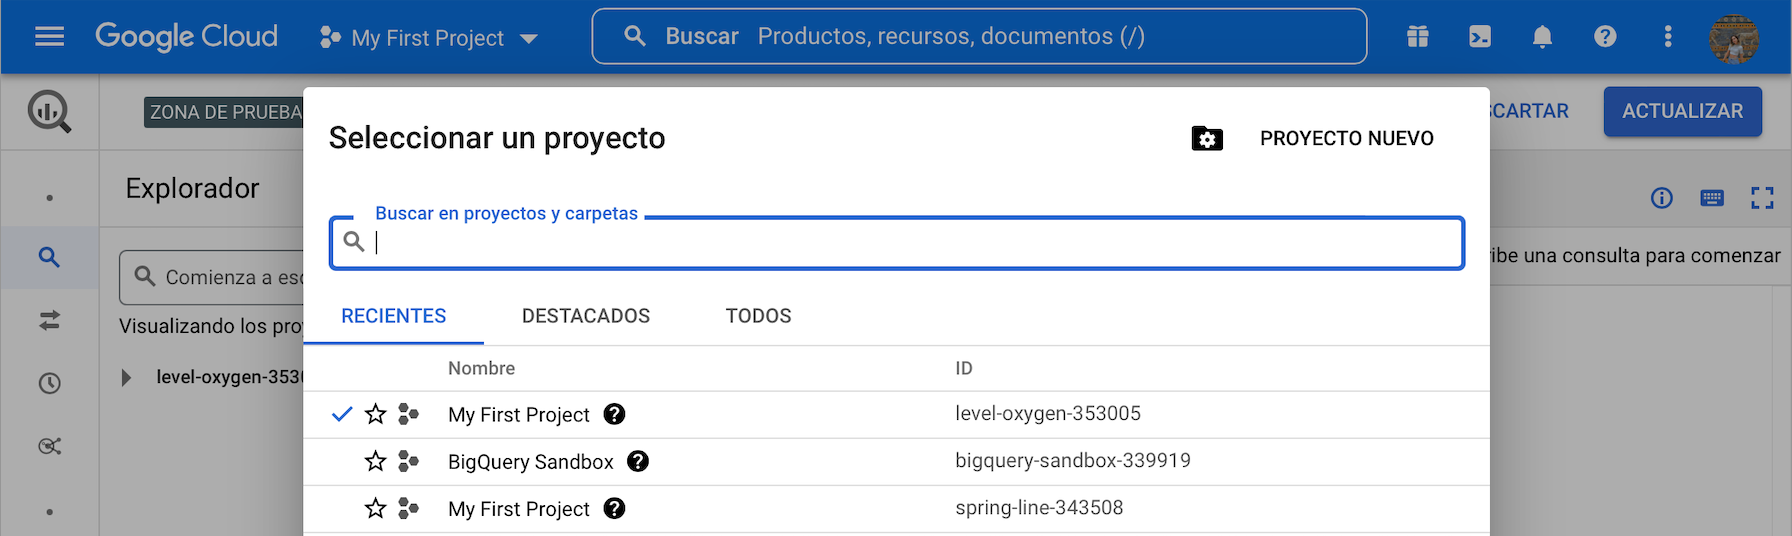
\includegraphics[width=7.25cm]{bq1}}%
\hfill
\raisebox{-.5\height}{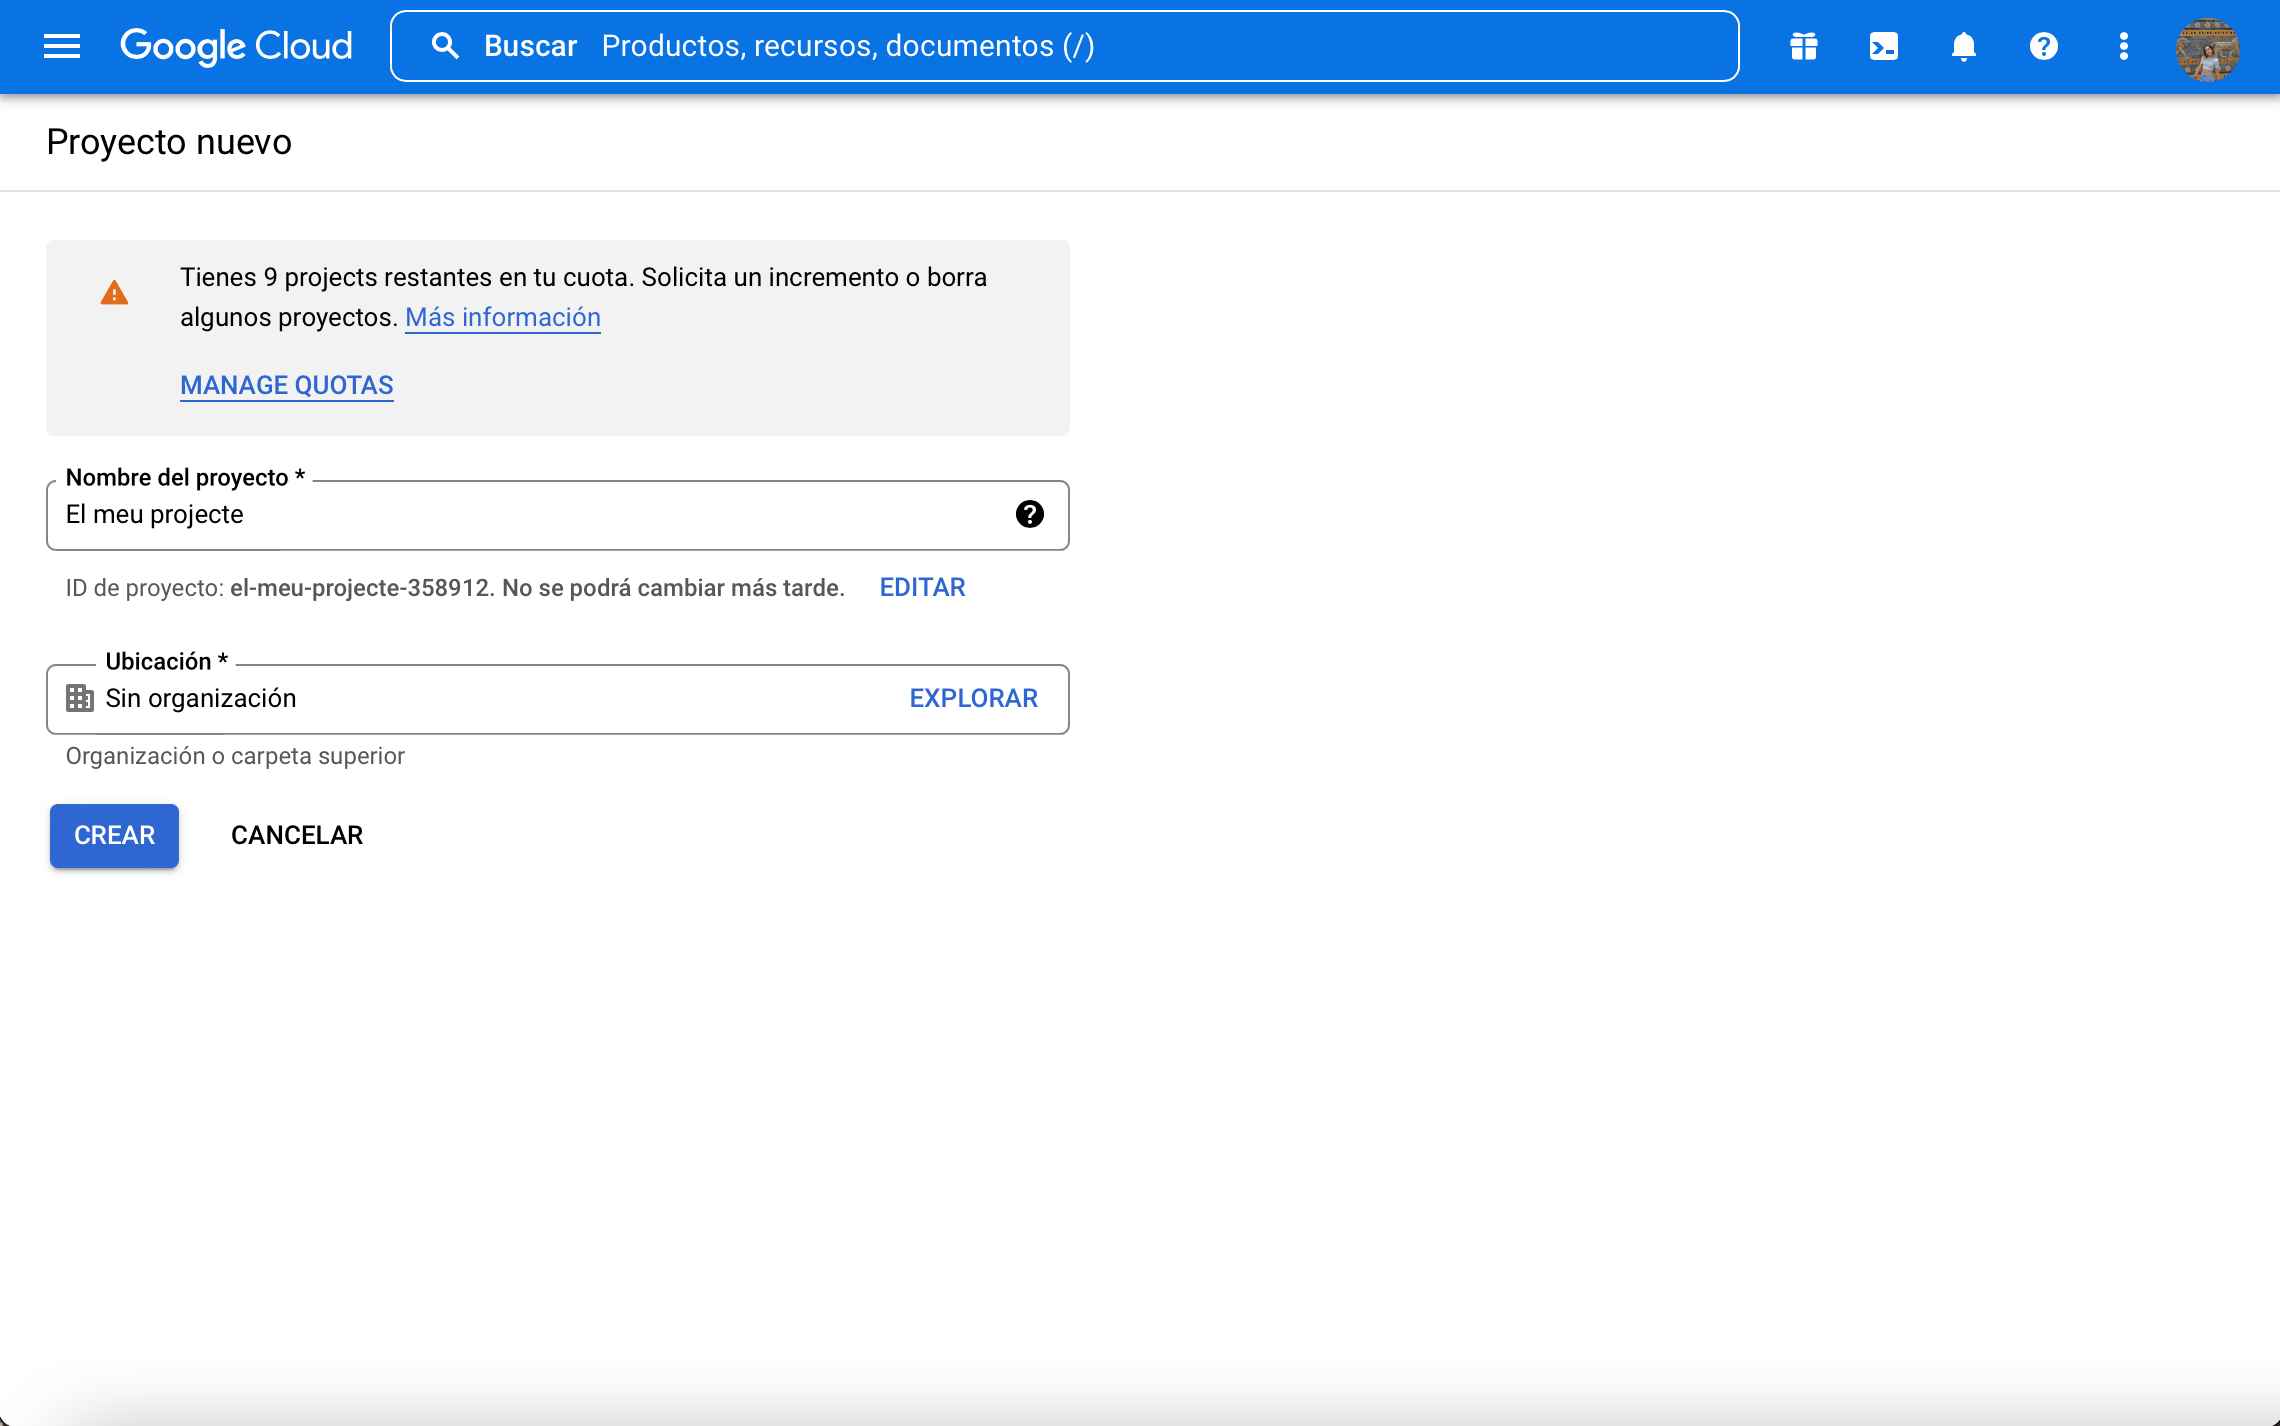
\includegraphics[width=7.25cm]{bq2}}%
\par
\caption{Creació d'un projecte}
\label{fig:bq1}
\end{figure}


4. Un cop creat el projecte, el navegador ens redirigeix a la interfície web de BigQuery.



5. Ara ja podrem carregar o consultar dades en el nostre projecte sense cap compte de facturació adjunta.

\subsubsection{Limitacions}

Això no obstant, per a l’ús de la zona de proves gratuïta que ofereix Google, haurem de tenir en compte un seguit de limitacions.



En primer lloc, ens trobem amb un màxim de 10 Gb d’emmagatzemament i 10 Tb de consulta al mes. Al llarg d’aquest exemple no utilitzarem un volum de dades més gran ni sobrepassarem el límit d’espai de consulta, però s’han de tenir en compte aquestes limitacions si l’objectiu és treballar amb el format gratuït.



A més, ens trobem que tots els conjunts de dades tenen el temps de caducitat de la taula per defecte establerta en seixanta dies. Per tant, totes les taules, vistes o particions de les taules caducaran automàticament passat aquest temps.



Una altra característica destacable és que els projectes de la zona de proves no són compatibles amb:

- La transmissió de dades.

- Sentències de llenguatge de manipulació de dades (DML).

- El servei de transferència de dades de BigQuery.

\subsection{Creació d'un conjunt de dades}

Ara que ja disposem d'un projecte en el qual treballar, ha arribat el moment de crear un nou conjunt de dades dins d'aquest. Es pot pensar en un conjunt de dades a BigQuery com una agrupació lògica de taules. Alhora, diferents conjunts de dades s'integren en un mateix projecte. 



Per a crear-ne un, només s'ha de desplegar el menú i triar l'opció de \texttt{crear un nou conjunt de dades}. Tot seguit, hi ha diversos detalls per al conjunt de dades que es poden establir. En primer lloc, hi ha l'opció de canviar el projecte que l'encabirà. Això farà que aparegui un navegador on es podrà especificar el projecte. Una altra possibilitat serà escollir la ubicació de les dades. Això determina on s'aprovisionaran els recursos subjacents, com la computació i l'emmagatzematge, per al servei BigQuery. Les consideracions a l'hora de triar una ubicació inclouran el rendiment per als usuaris finals, l'alta disponibilitat i també qualsevol restricció d'auditoria o compliment. I, per últim, es pot establir un temps d'expiració per defecte per a les taules dins d'un conjunt de dades.


\begin{figure}[h!]
\par
\raisebox{-.5\height}{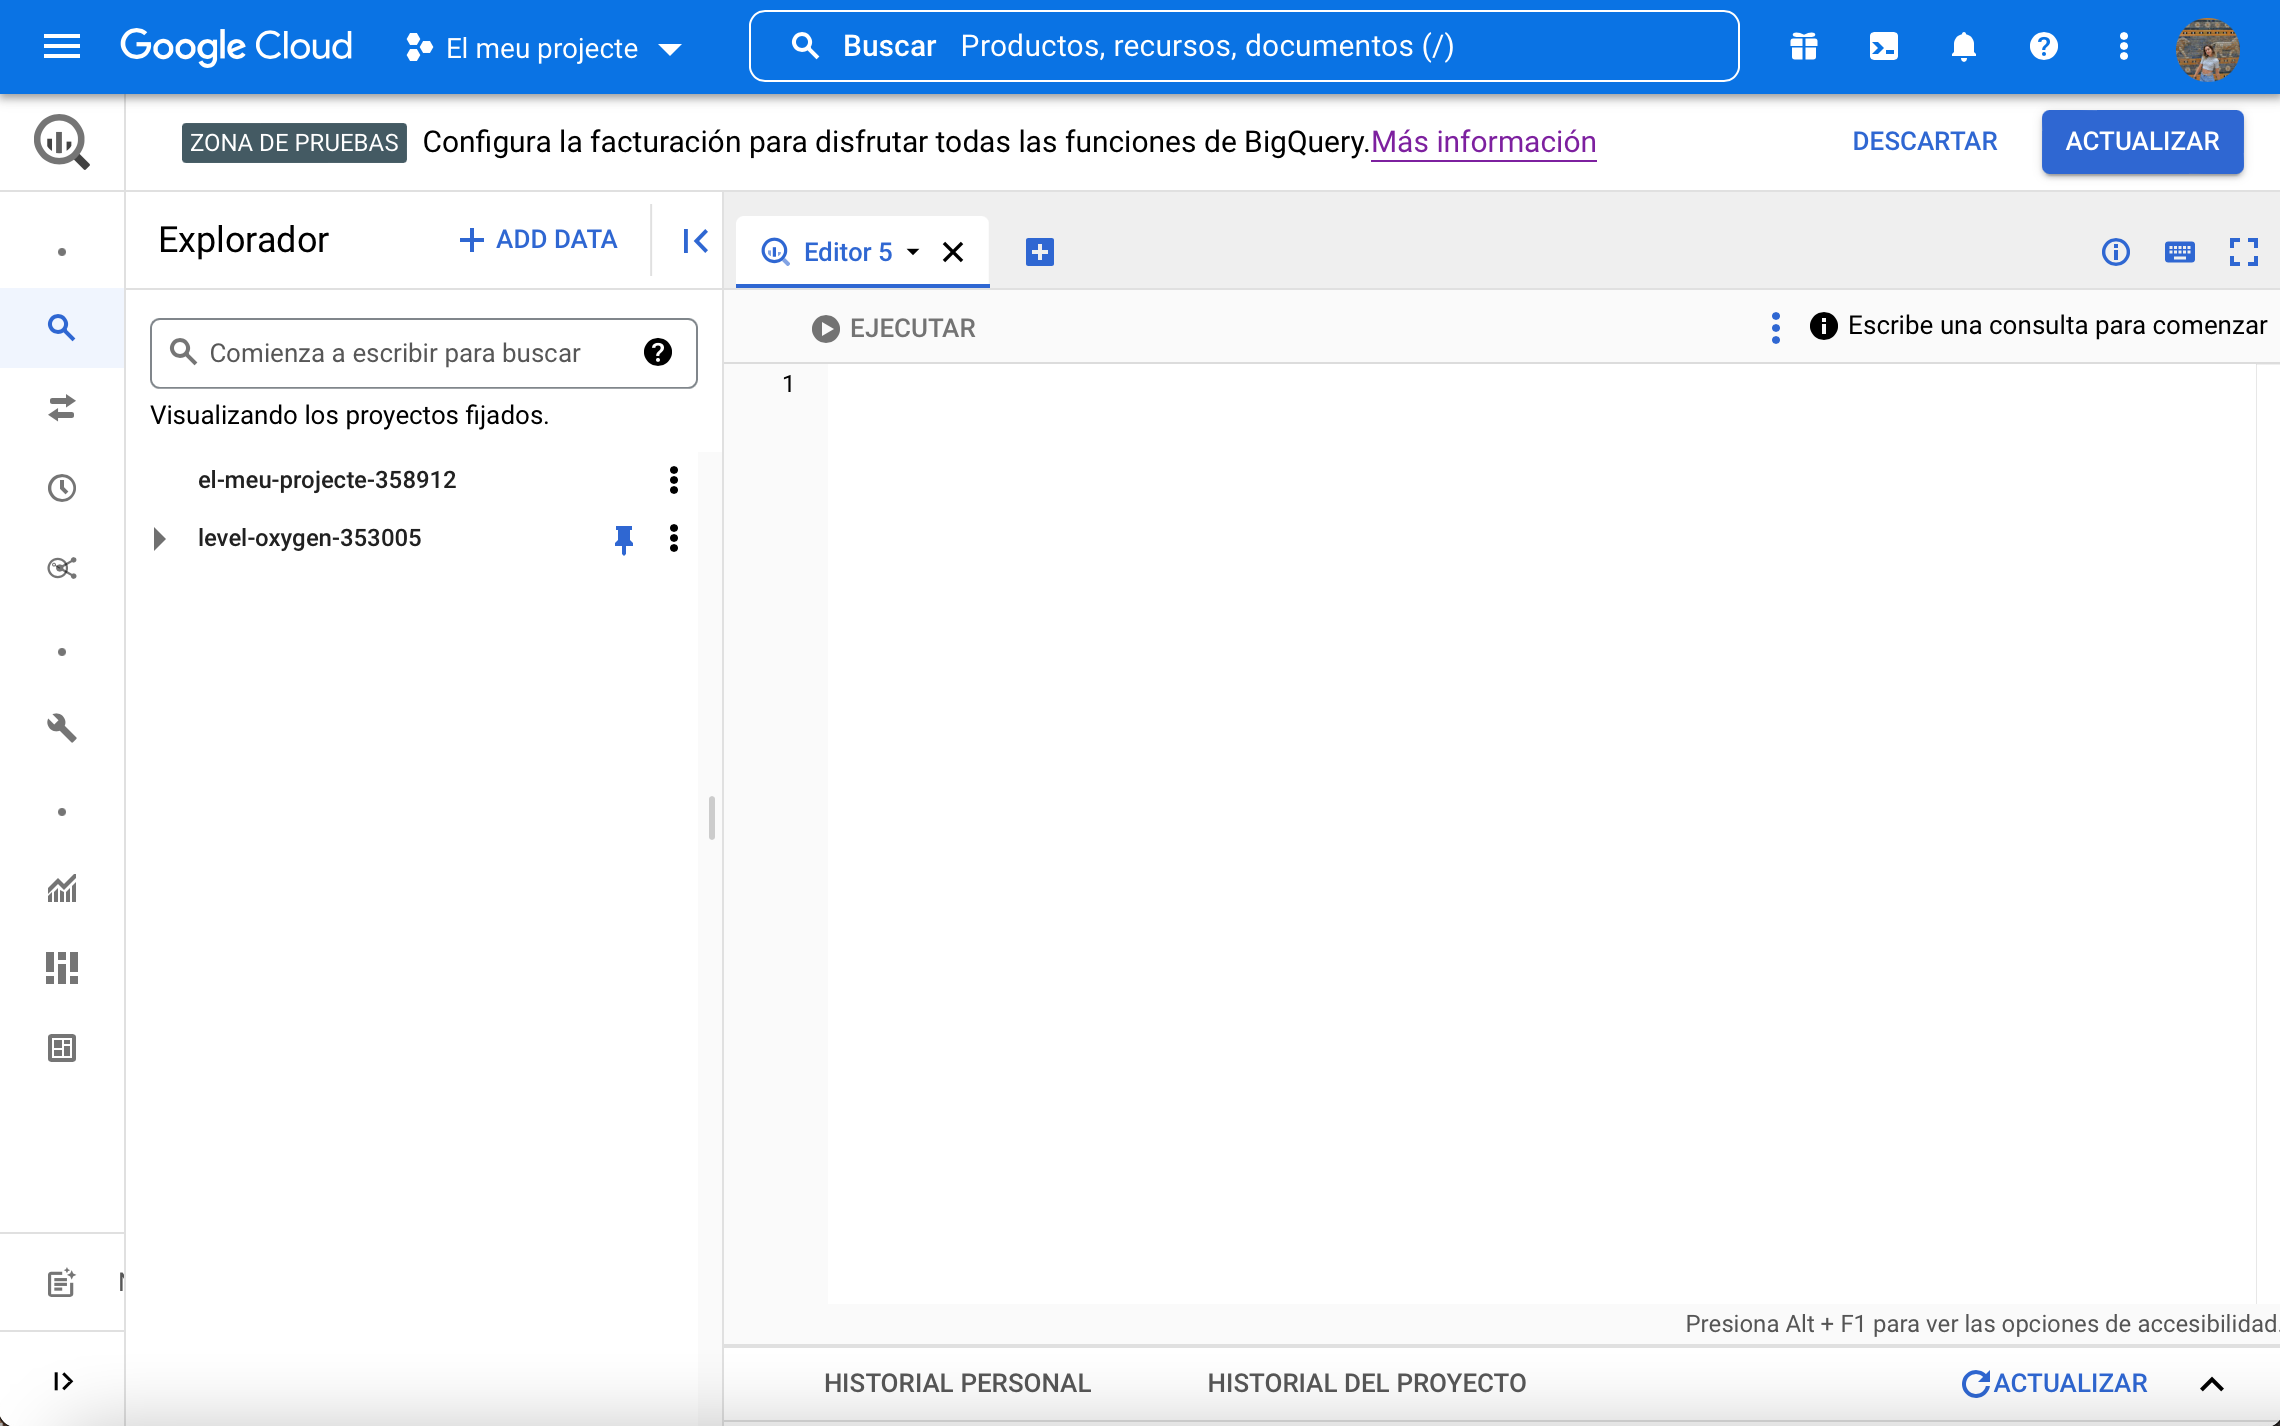
\includegraphics[width=7.25cm]{bq3}}%
\hfill
\raisebox{-.5\height}{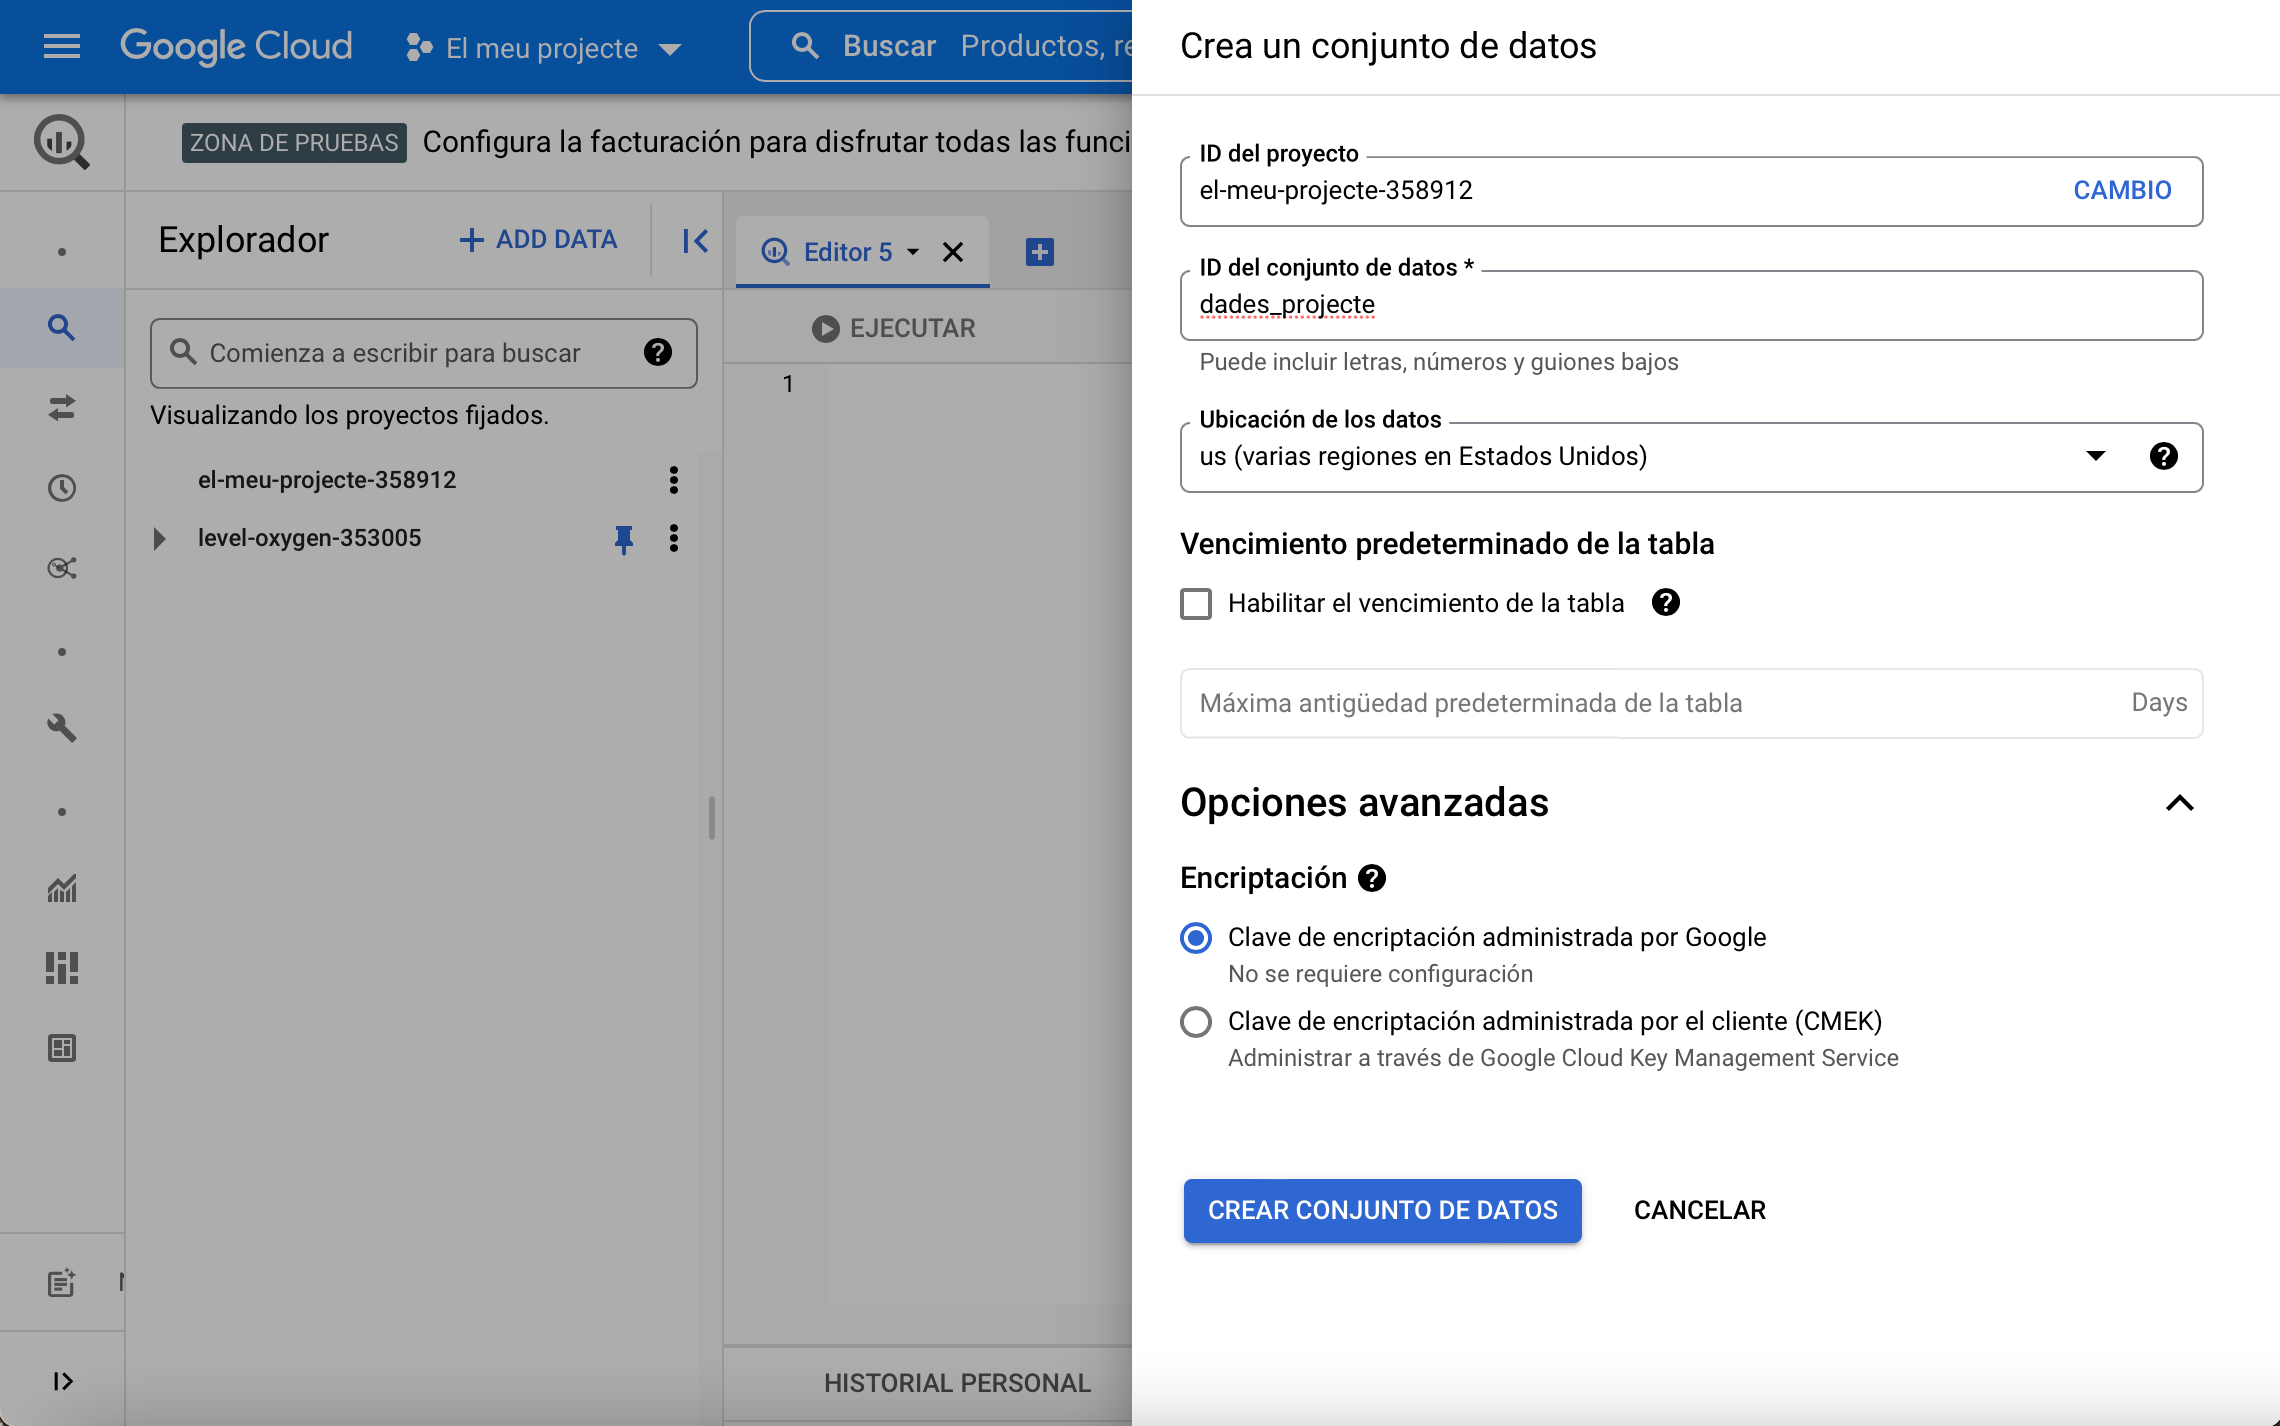
\includegraphics[width=7.25cm]{bq4}}%
\par
\caption{Creació d'un conjunt de dades}
\label{fig:bq3}
\end{figure}


Tal com es pot veure a la figura ~\ref{fig:bq3}, hem creat un nou conjunt de dades anomenat \verb|dades_projecte| que estarà ubicat en el projecte \verb|el_meu_projecte|, la ubicació de les dades l'hem posat a diverses regions dels Estats Units i, per últim, no hem habilitat un temps de venciment de la taula, sinó que per defecte BigQuery l'emmagatzemarà per 60 dies.


\begin{figure}[h!]
\begin{center}
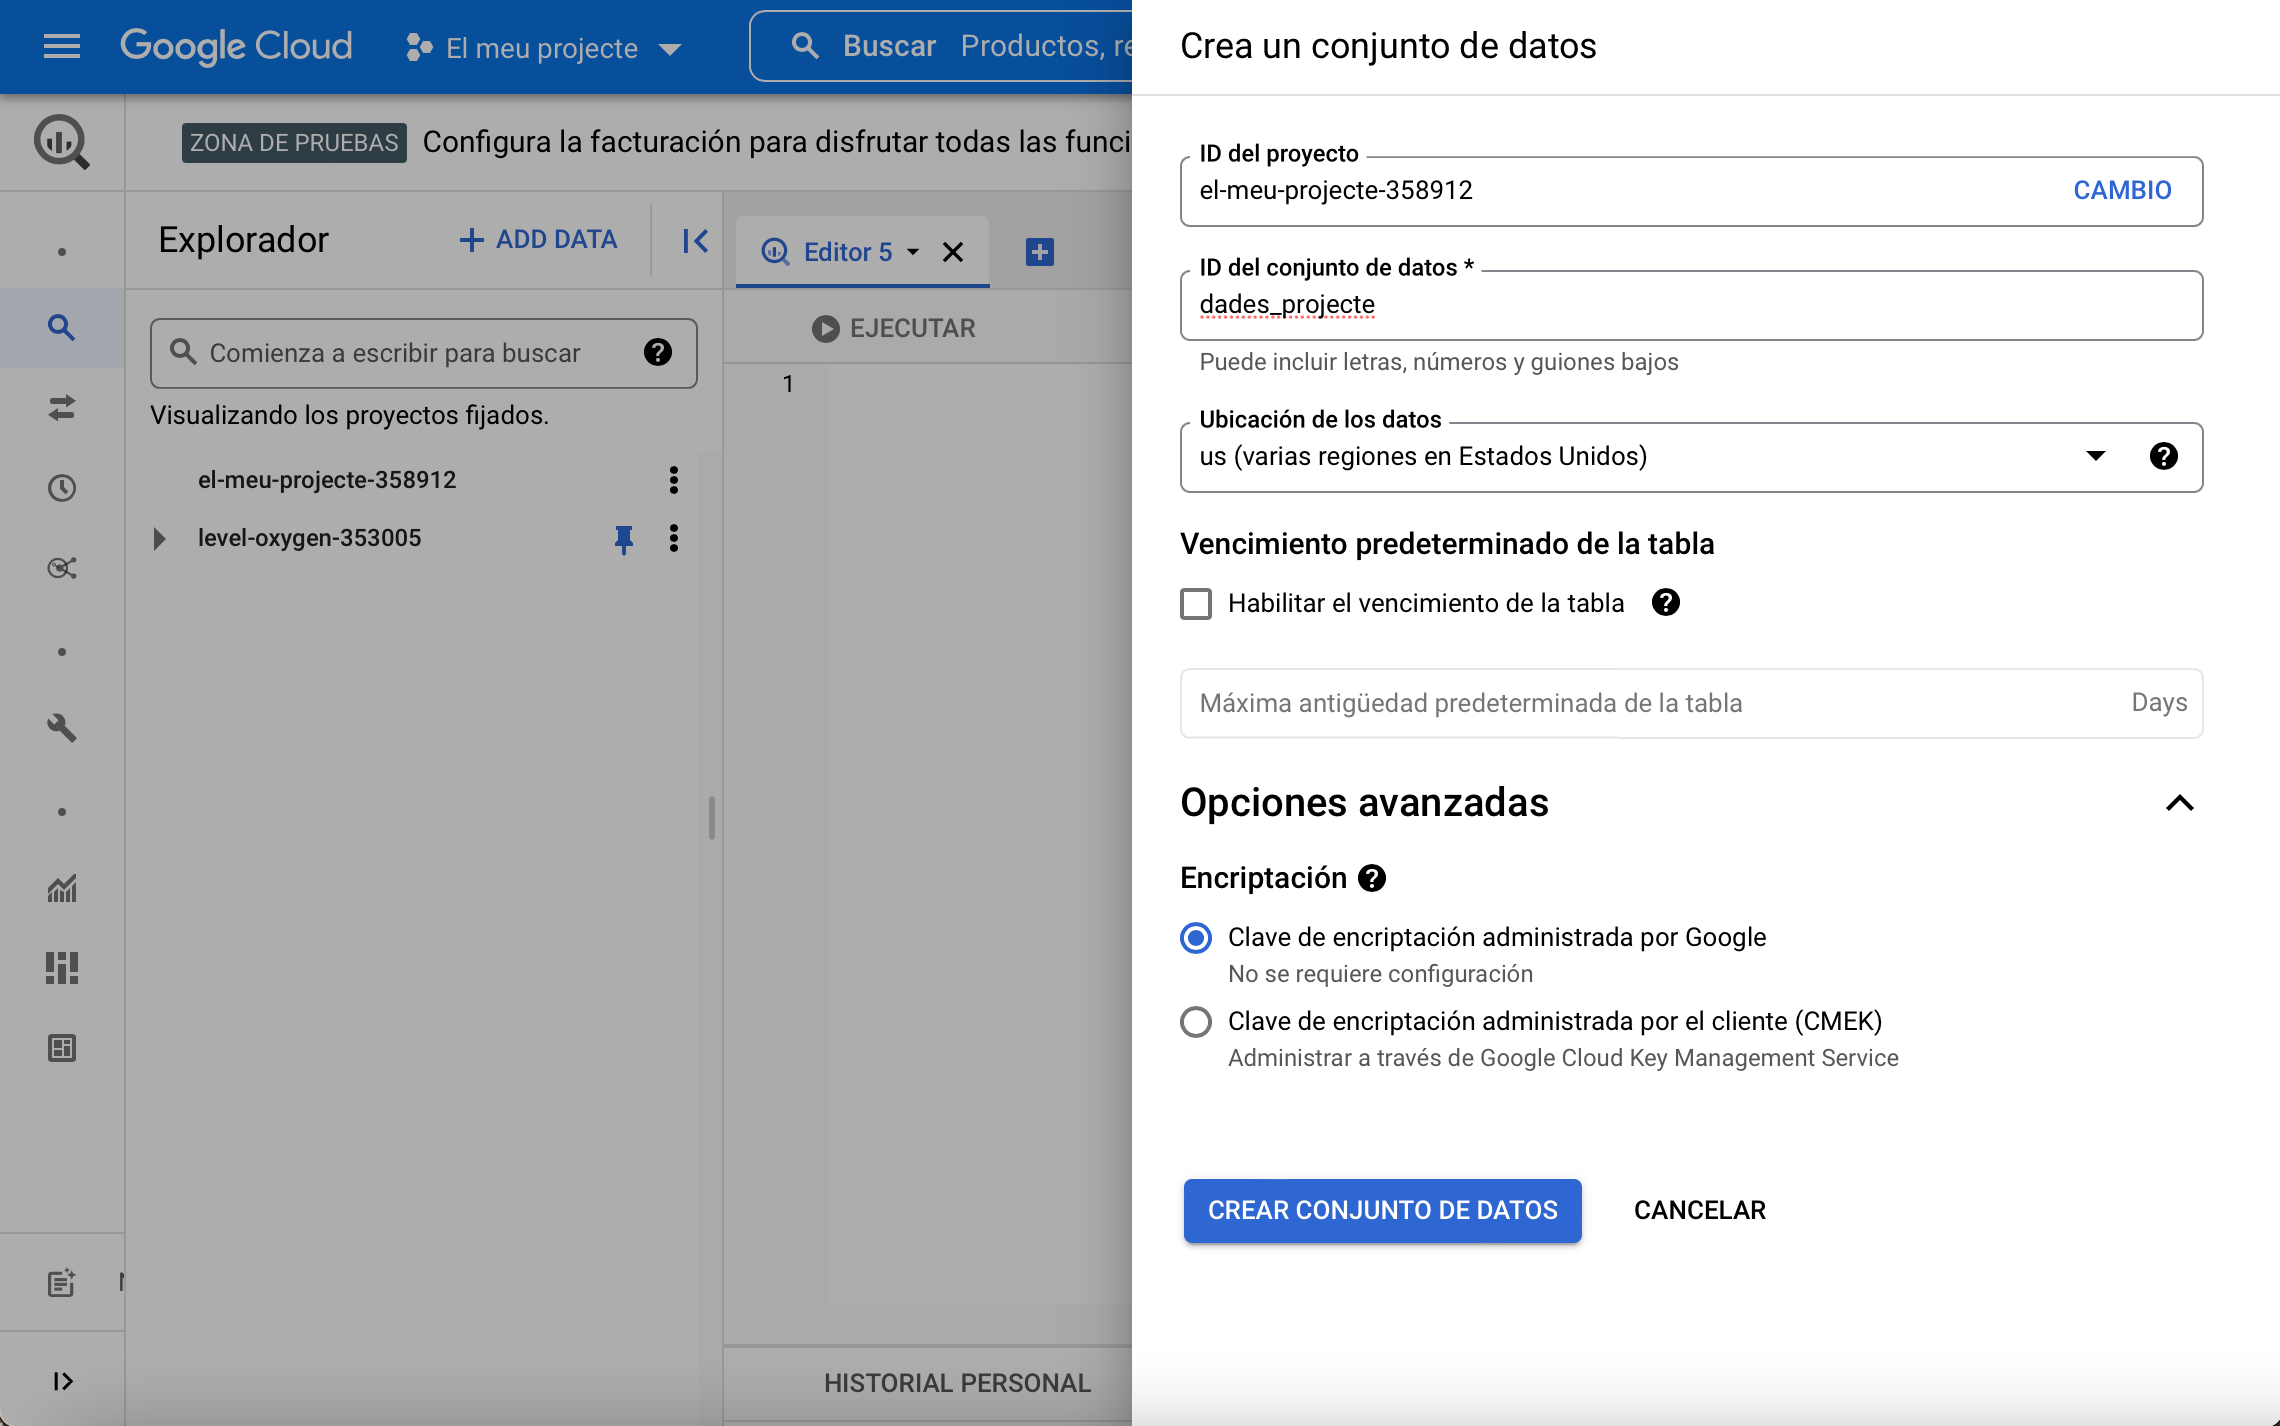
\includegraphics[width=10cm]{bq5}
\end{center}
\caption{Informació del conjunt de dades}
\label{fig:bq5}
\end{figure}


Un cop creat \verb|dades_projecte|, es pot comprovar que ara apareix dins de \verb|el_meu_projecte| a la interfície d'usuari (UI) de BigQuery, i s'observa que no hi ha taules dins d'aquest. També es pot donar un cop d'ull als detalls associats a aquest conjunt de dades (Figura ~\ref{fig:bq5}). Des d'aquest menú, podem triar obrir-lo, i es desplegarà a la dreta tota la informació del conjunt de dades. Aquí podem confirmar l'identificador del conjunt de dades, que també assenyala el projecte en el qual s'ha creat el conjunt de dades, i després altres detalls que inclouen les hores de creació i modificació, així com la ubicació d'aquest.



A més, des d'aquesta finestra podrem compartir el conjunt de dades amb altres usuaris. Hi ha opcions per a copiar i eliminar aquest conjunt de dades. I després, a l'opció \textit{editar detalles}, podem reconfigurar el temps de caducitat de les taules, establir una descripció o afegir etiquetes. Per exemple, si volem marcar aquest conjunt de dades com a pertanyent a un equip, podem establir una etiqueta amb la clau d'equip i el valor corresponent. En acabant, quan el guardem, les etiquetes apareixen a l'apartat d'informació.

\subsection{Definició d'una taula de BigQuery des de la interfície d'usuari}

Després d'haver creat un conjunt o base de dades en un projecte, ja es pot crear una taula dins d'ell. Si tenim la informació de la base, hauríem de veure aquesta opció per a crear una nova taula des d'aquí. Alternativament, podem dirigir-nos al projecte, després al conjunt de dades i triar l'opció de crear una taula. Apareixerà un formulari i tindrem l'opció d'especificar una font per a la nostra taula. Això ens permetrà importar dades de fonts ja existents, com l'emmagatzematge en el núvol de Google o bé un arxiu dels nostres propis sistemes. La primera taula que crearem serà bastant simple, i ens servirà per explorar una mica la plataforma. De fet, serà una taula buida anomenada \verb|accidents| (Figura ~\ref{fig:bq6}). 


\begin{figure}[h!]
\par
\raisebox{-.5\height}{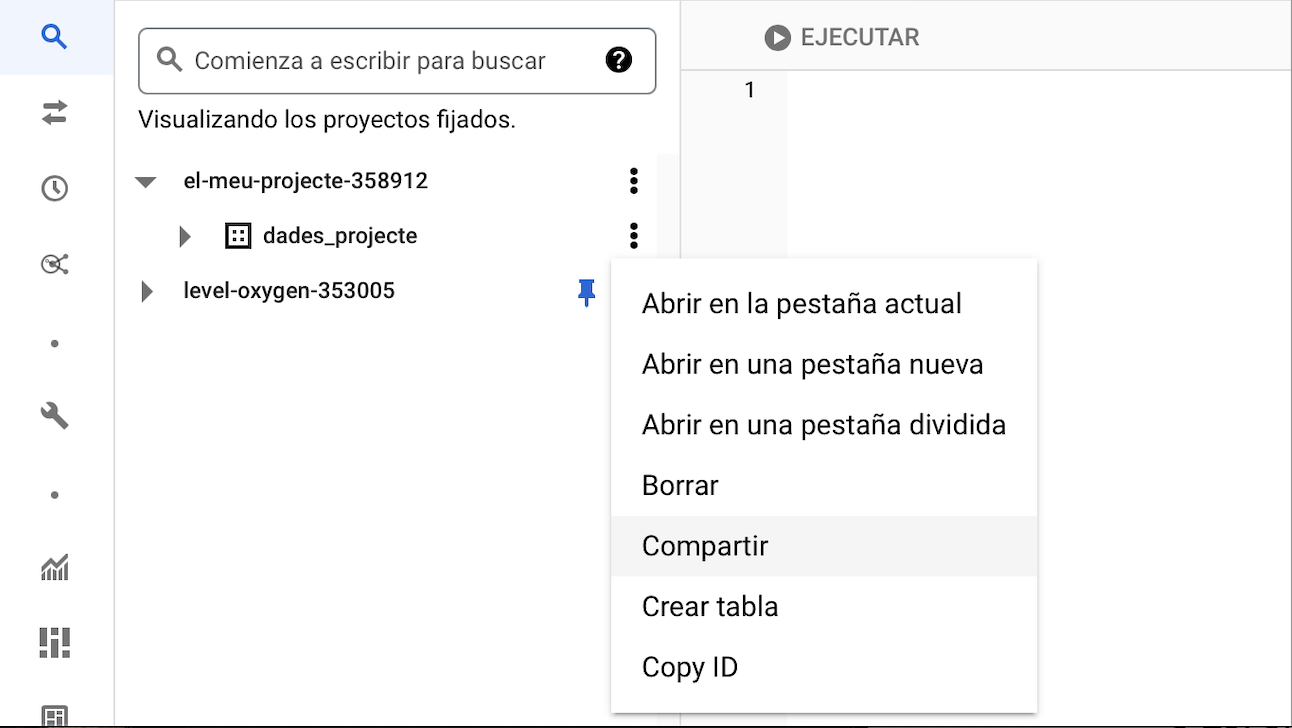
\includegraphics[width=7.25cm]{bq6}}%
\hfill
\raisebox{-.5\height}{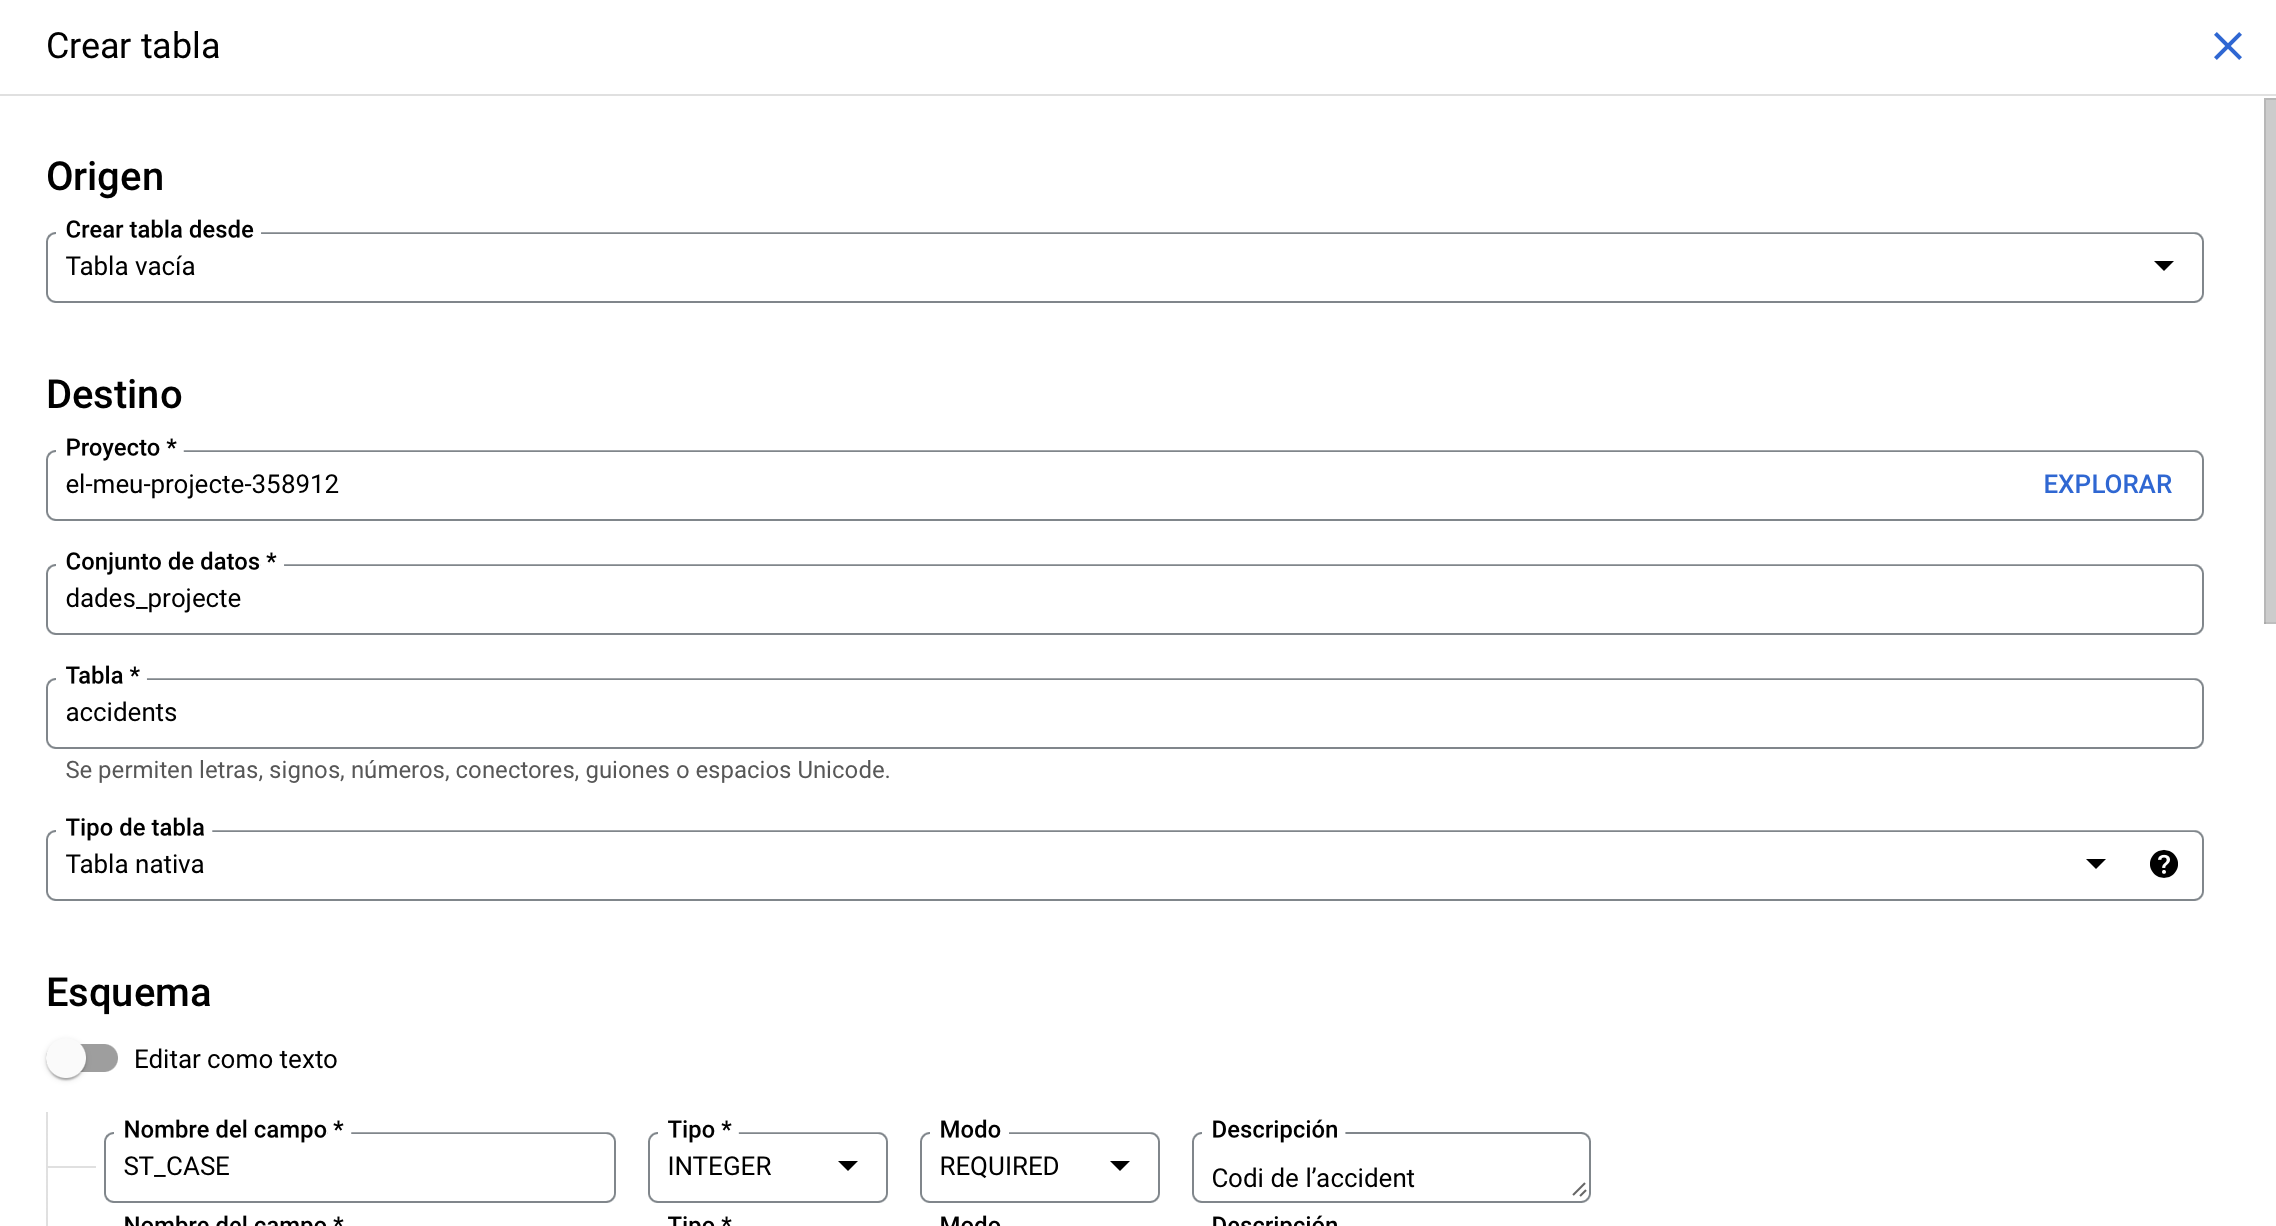
\includegraphics[width=7.25cm]{bq7 copia}}%
\par
\caption{Creació d'una taula}
\label{fig:bq6}
\end{figure}


A continuació, passem a la secció d'Esquema. Podem fer ús d'aquesta interfície per a establir les columnes de la nostra taula, incloent-hi els tipus i altres configuracions. La primera columna que definirem és l'identificador de l'accident, que s'anomenarà \verb|ST_CASE|. Per al tipus de variable, podem triar d'entre menú d'opcions, que inclou tots els tipus amb els quals ja estem familiaritzats. Quant a la manera (columna \textit{modo} a la figura ~\ref{fig:bq8}), aquesta determinarà si els valors d'aquesta columna poden ser nuls o si es requereix un valor (com és el cas de l'identificador), i també podem establir que els valors siguin d'un tipus que es pugui repetir, marcant \textit{indistint}. Finalment, es pot escriure una descripció per a la variable, que és opcional. 


\begin{figure}[h!]
\begin{center}
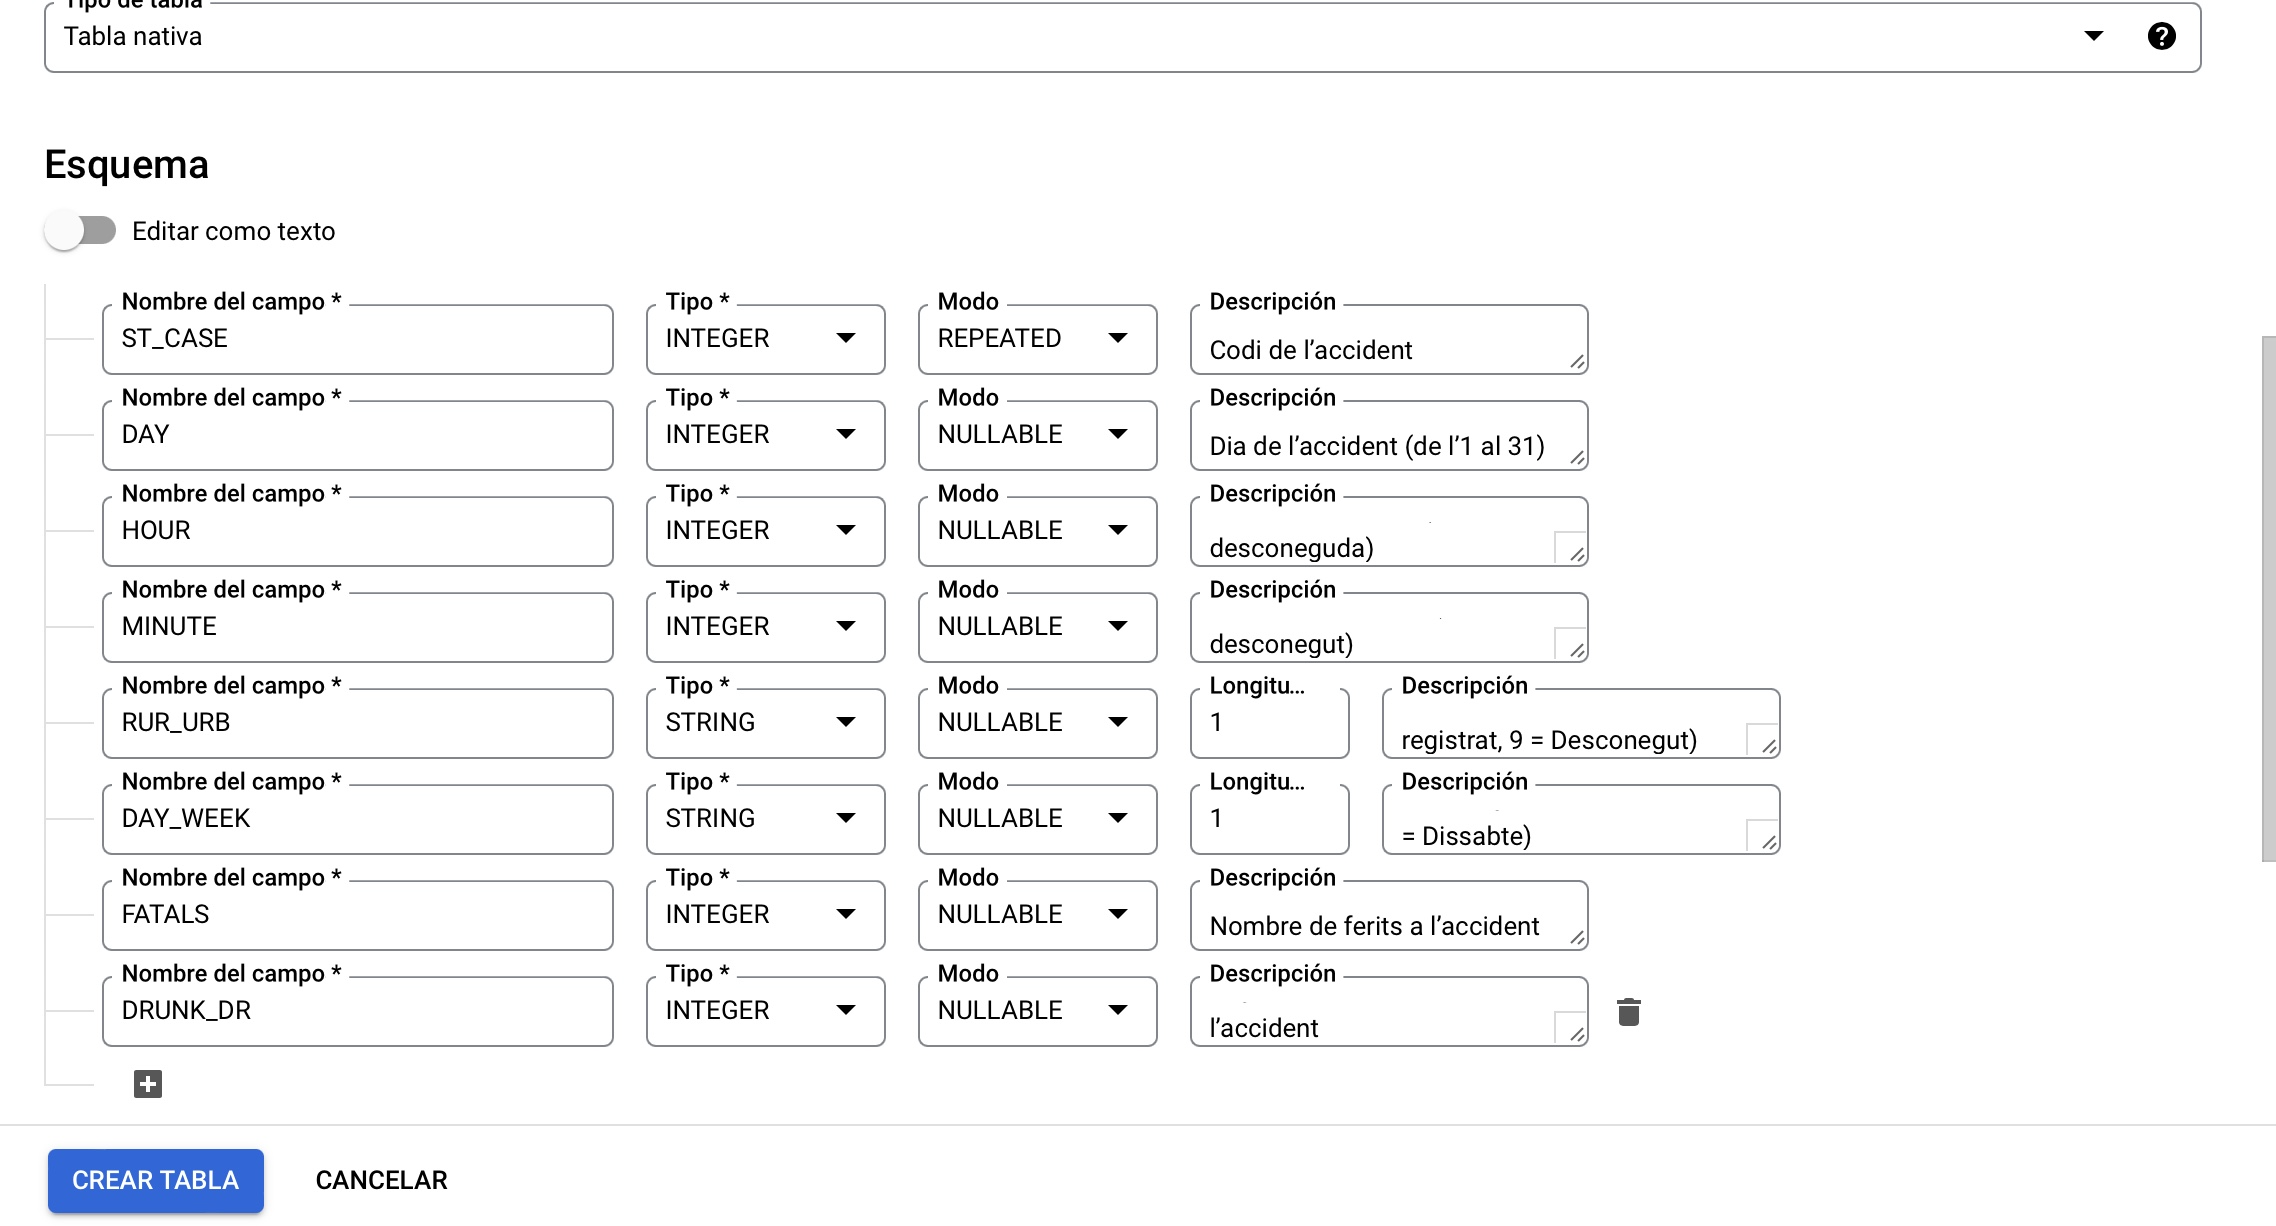
\includegraphics[width=10cm]{bq8}
\end{center}
\caption{Esquema de la nostra taula}
\label{fig:bq8}
\end{figure}


La taula ~\ref{tab:taula1} que acabem de crear està formada per 8 variables, 6 de les quals són numèriques i 2 categòriques, i es descriuen tal com es pot veure a continuació.

\begin{table}[h]
\resizebox{\textwidth}{!}{%
\begin{tabular}{|l|l|l|}
\hline
\textbf{Variable}  & \textbf{Tipus}      & \textbf{Descripció}                                                                                                        \\ \hline
ST\_CASE       & Numèrica & Codi de l'accident                                                                                   \\ \hline
DAY       & Numèrica & Dia de l’accident (de l’1 al 31)                                                                                    \\ \hline
HOUR      & Numèrica   & Hora de l’accident (99 = desconeguda)                                                                               \\ \hline
MINUTE    & Numèrica   & Minut de l’accident (99 = desconegut)                                                                               \\ \hline
RUR\_URB  & Categòrica & Informació sobre la localització (1 = Rural, 2 = Urbà,   \\ 
& & 6 = Via no classificada, 8 = No registrat, 9 = Desconegut) \\ \hline
DAY\_WEEK & Categòrica & Dia de la setmana (1 = Diumenge, 2 = Dilluns, ..., 7 = Dissabte)                                                    \\ \hline
FATALS    & Numèrica   & Nombre de víctimes a l’accident (poden der ferits o morts)                                                                                      \\ \hline
DRUNK\_DR & Numèrica   & Nombre de conductors beguts involucrats a l’accident                                                                \\ \hline
\end{tabular}%
}
\caption{Especificacions de la taula Accidents}
\label{tab:taula1}
\end{table}



En el transcurs del treball, farem ús d'aquesta taula, juntament amb dues més, que prenen de nom de \verb|persones| i \verb|vehicles|, per analitzar les dades que es van prendre d'un conjunt d'accidents de trànsit que es van donar a Washington, Estats Units durant el mes de desembre de l'any 2015. L'agència estatal de trànsit va fer públiques aquestes dades al seu portal web (\url{https://www.transportation.gov/briefing-room/traffic-fatalities-sharply-2015})

\subsubsection{Afegir dades a una taula de BigQuery senzilla}

Ara que hem creat una taula de consulta, podem centrar-nos a treballar amb ella. Per a això, ens desplaçarem cap avall i donarem un cop d'ull al primer esquema de la taula (a la figura ~\ref{fig:bq9}), on es troba a alguna informació interessant. Més enllà de la identificació de la taula, a l'esquerra de la figura, també podem comprovar la grandària de la taula a la dreta, que ens donarà una indicació de la quantitat de dades que es processarien en cas d'executar consultes sobre aquesta. La grandària d'emmagatzematge a llarg termini assenyala les dades a les quals no s'ha accedit en els últims 90 dies, i després, per descomptat, tenim les hores de creació i modificació, juntament amb la ubicació de les dades de la taula. Des d'aquesta interfície també podem editar els detalls existents d'aquesta taula. Aquí podem establir un temps de caducitat en cas que vulguem anul·lar el que s'ha establert en el nivell del conjunt de dades. També hi ha l'opció d'establir una descripció o afegir etiquetes.


\begin{figure}[h!]
\par
\raisebox{-.5\height}{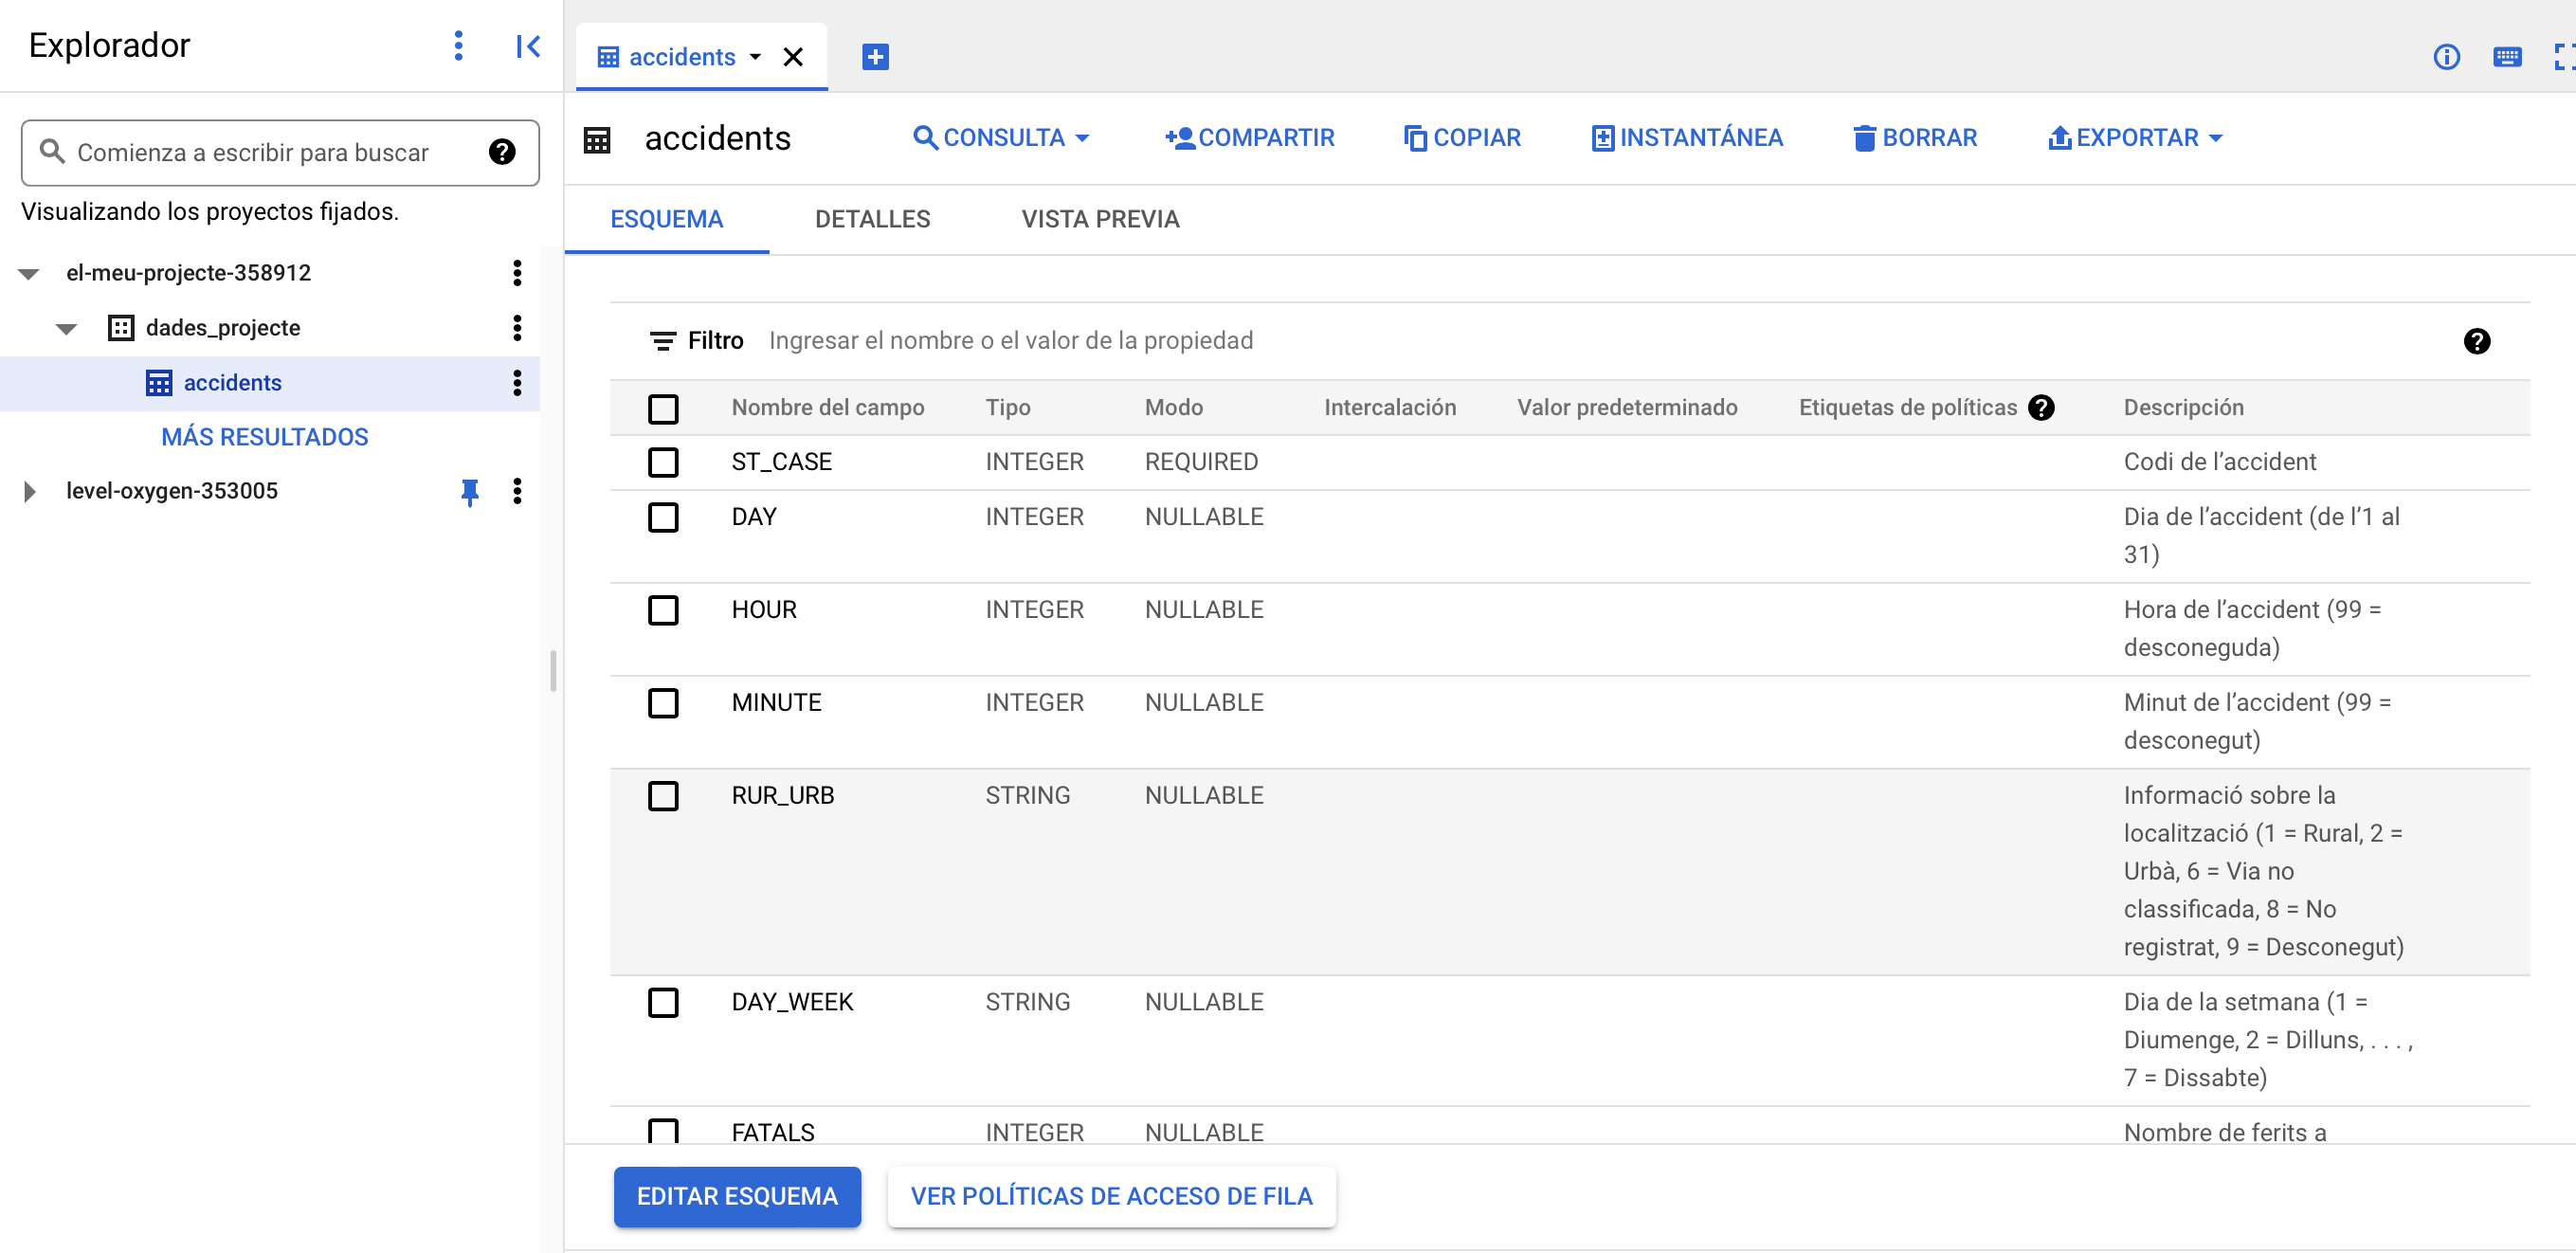
\includegraphics[width=7.25cm]{bq9}}%
\hfill
\raisebox{-.5\height}{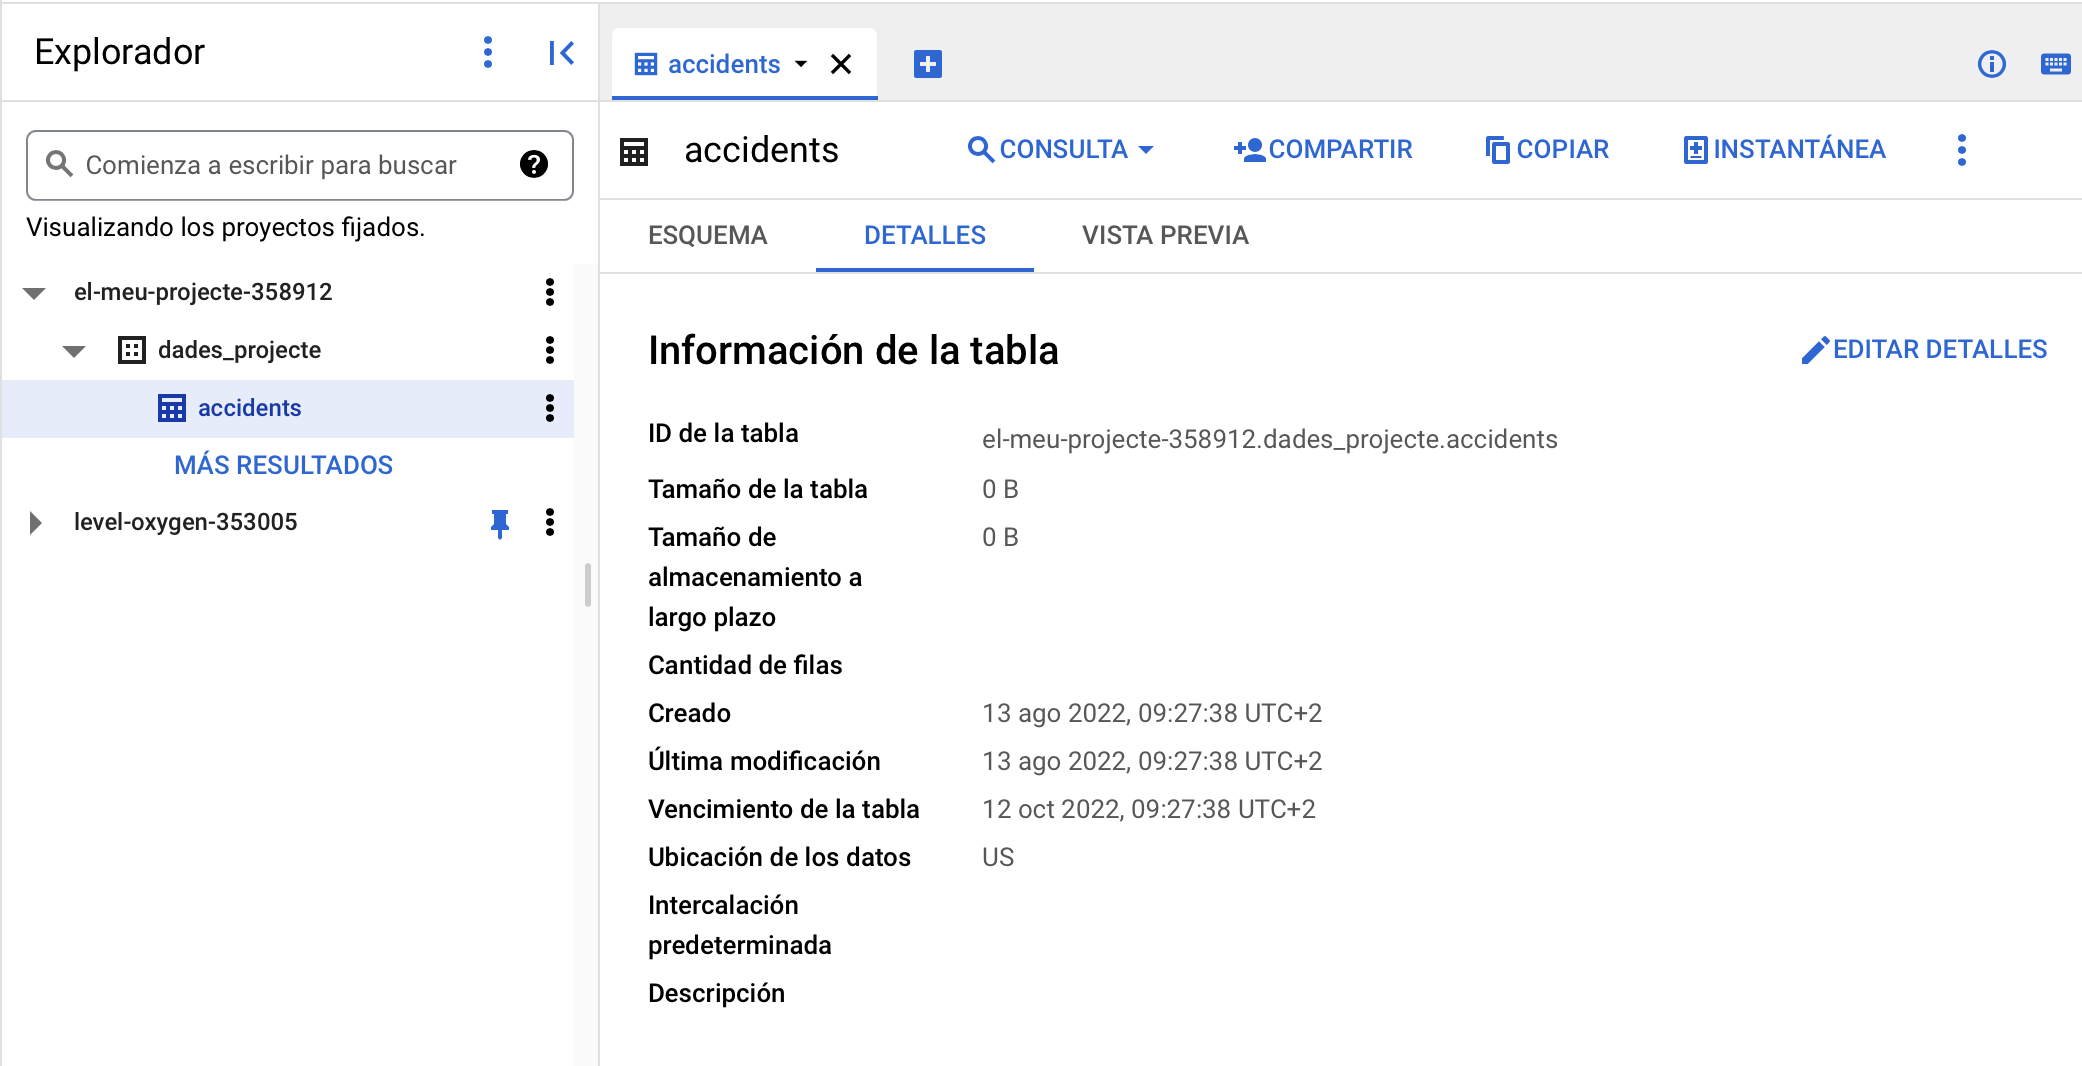
\includegraphics[width=7.25cm]{bq10}}%
\par

\caption{Detalls de la taula}
\label{fig:bq9}
\end{figure}


Una altra característica que podem consultar és la vista prèvia de la taula, i com és lògic, veurem que aquesta encara no conté dades, ja que simplement hem creat l'esquema de la taula, sense inserir cap dada en aquesta. Si féssim ús de SQL, en qualsevol altre context es podrien afegir dades a partir d'una simple consulta a la taula, que tindria l'estructura següent:

\begin{verbatim}
INSERT INTO `el-meu-projecte-358912.dades_projecte.accidents` 
(ST_CASE, DAY, HOUR, MINUTE, RUR_URB, DAY_WEEK, FATALS, DRUNK_DR)
VALUES (20055, 1, 20, 55, "1", "3", 3, 0);
\end{verbatim}

A partir d'aquesta consulta afegiríem a la taula el cas d'un accident amb identificador 20055, que es va produir el dia 1 del mes a les 20:55 a una zona rural (\verb|RUR_URB| = 1) un dimarts (\verb|DAY_WEEK| = 3), i en el que hi ha 3 víctimes i cap conductor begut involucrat en l'accident.

Això no obstant, quan intentem executar la consulta, BigQuery ens informa d'un error (Figura ~\ref{fig:bq11}). Si recordem, prèviament s'han definit algunes de les limitacions per a l'ús de la zona de proves de BigQuery. Entre aquestes s´hi troba que no podem utilitzar el llenguatge de manipulació de dades (DML), és a dir, que no podem modificar la taula amb sentències com \verb|INSERT INTO|, \verb|UPDATE| o \verb|DELETE|, per exemple. Per aquest motiu, l'error ens avisa que no tenim el nostre projecte vinculat a un compte i, per tant, no ens avaluarà la nostra consulta.


\begin{figure}[h!]
\begin{center}
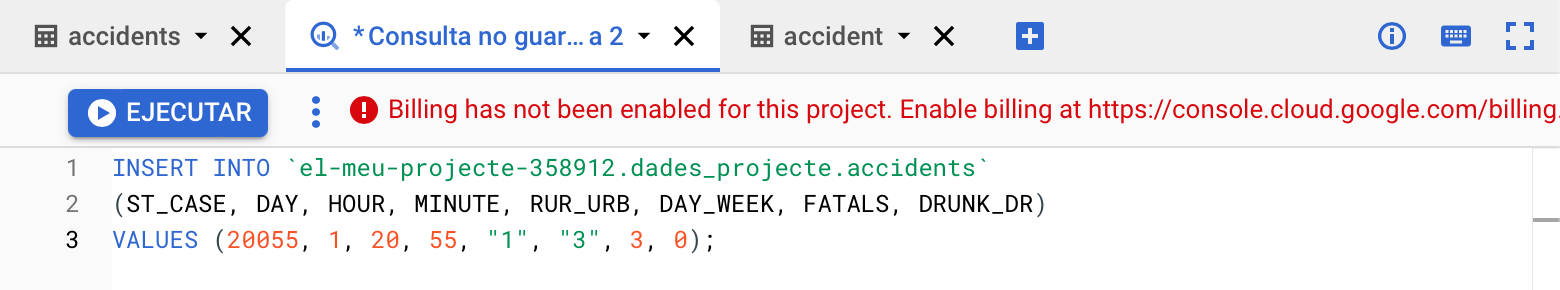
\includegraphics[width=12cm]{bq11}
\end{center}
\caption{Inserció de dades a la taula}
\label{fig:bq11}
\end{figure}


\newpage

\subsection{Càrrega de dades per crear una taula de BigQuery}

Ara explorarem un cas d'ús més comú per als usuaris de BigQuery, que tracta de crear una taula a partir de dades existents. Per a això, ens dirigirem al nostre conjunt de dades, \verb|dades_projecte|, i triarem crear una nova taula. Aquest cop, la font no serà una taula buida, sinó que carregarem un arxiu CSV del nostre propi sistema d'arxius. Un cop seleccionem importar les dades, es pot seleccionar diferents tipus d'arxiu com ara CSV, JSON, Avro o Parquet, principalment. Per a respectar les limitacions de la zona de proves, hi ha algunes restriccions quant a la grandària de l'arxiu que podem pujar, recordem que aquestes han de ser menors a 10 Gb. Procedim llavors a navegar pels nostres sistemes d'arxius per a l'arxiu a pujar. Una vegada que l'arxiu ha estat seleccionat, el format de l'arxiu s'ha establert automàticament en CSV (Figura ~\ref{fig:bq12}). 


\begin{figure}[h!]
\par
\raisebox{-.5\height}{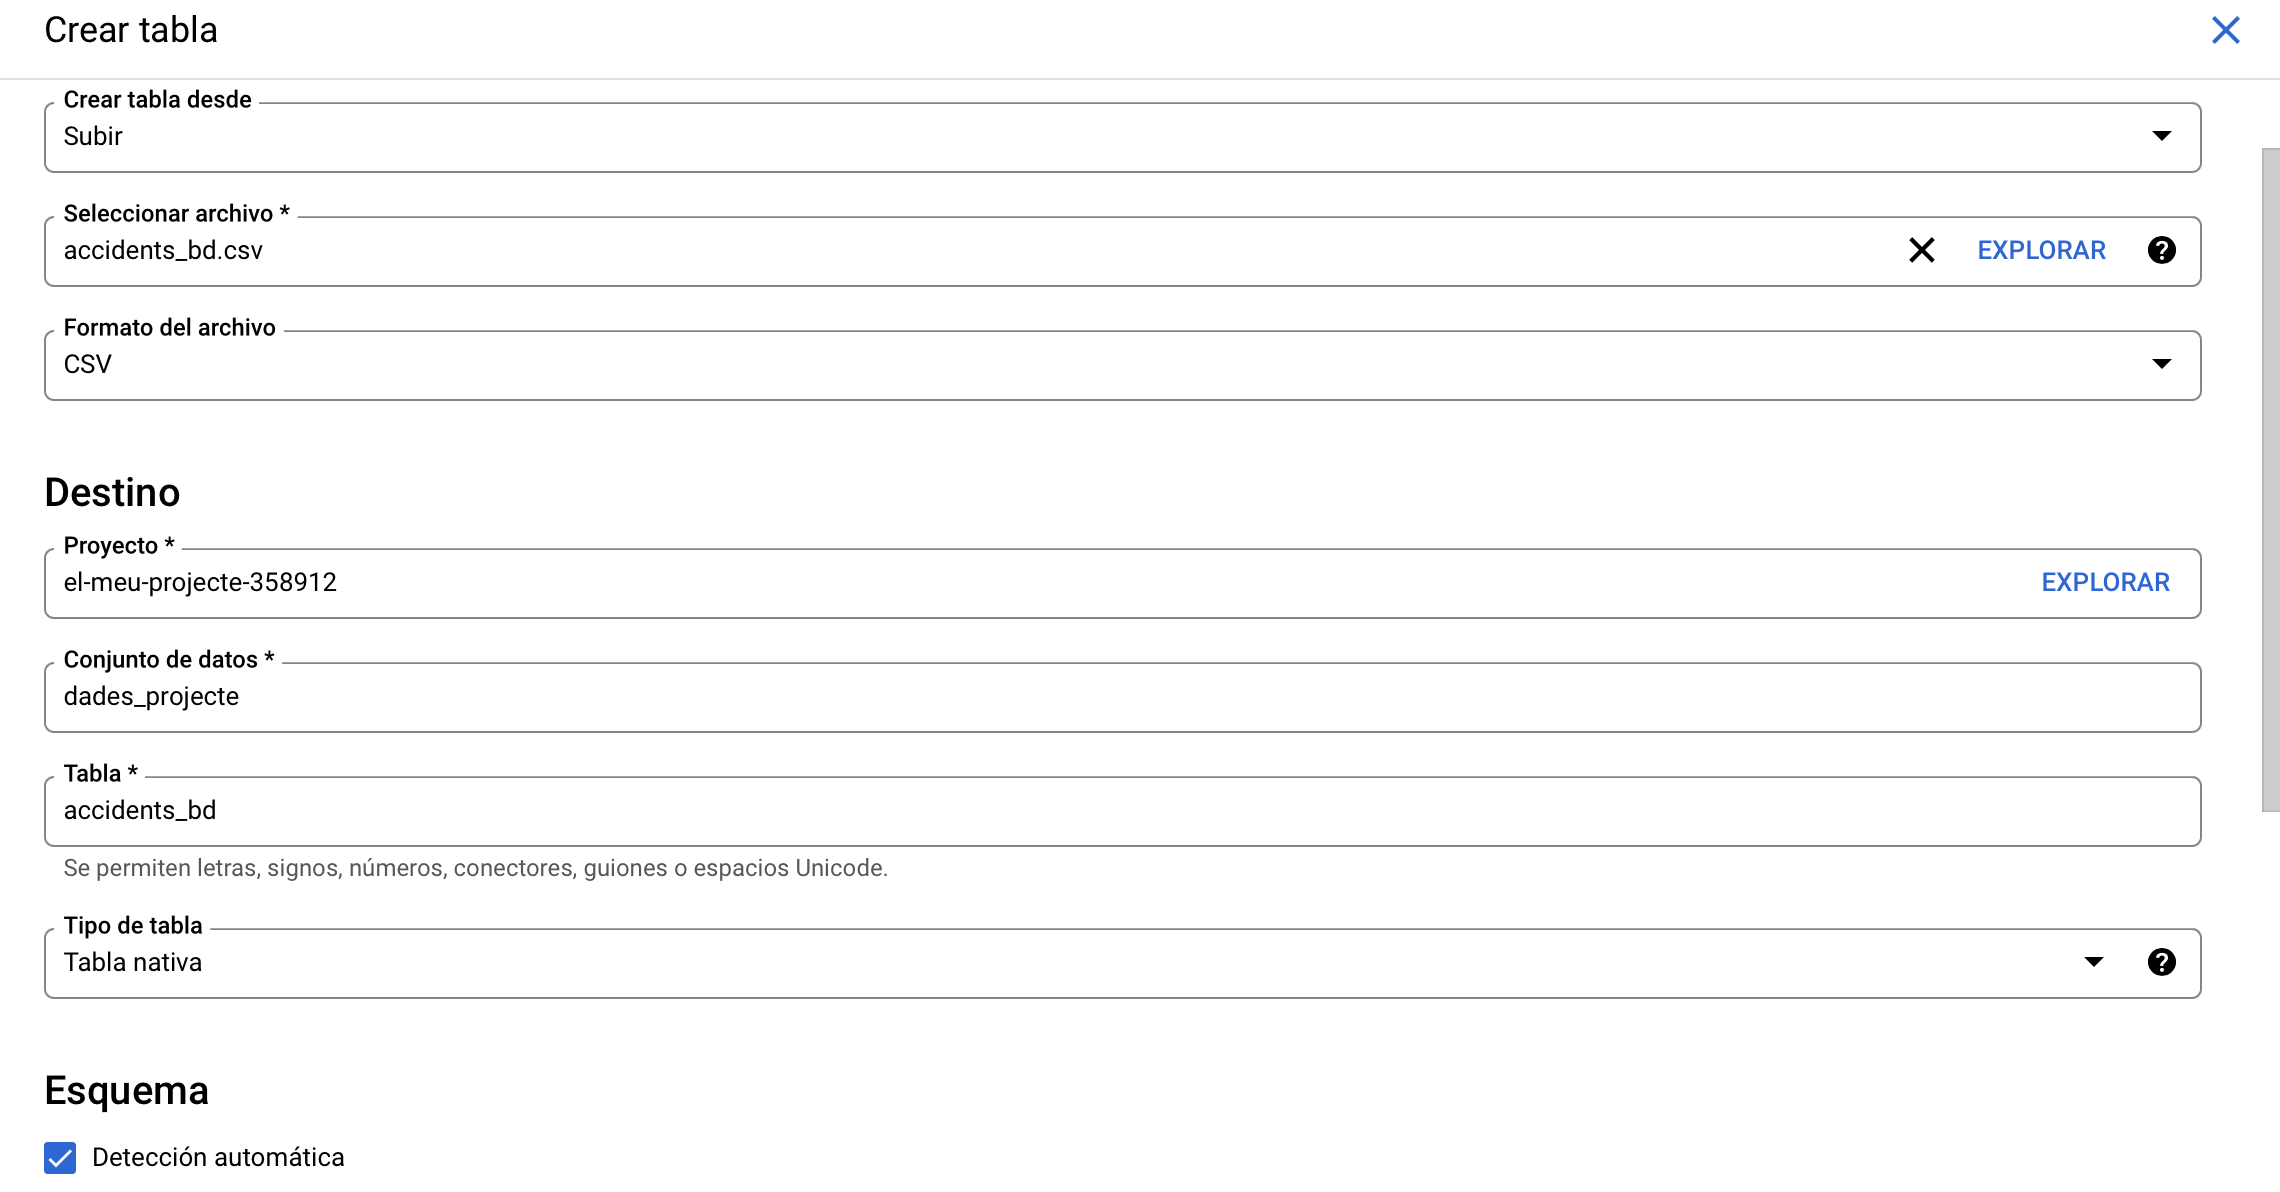
\includegraphics[width=7.25cm]{bq12}}%
\hfill
\raisebox{-.5\height}{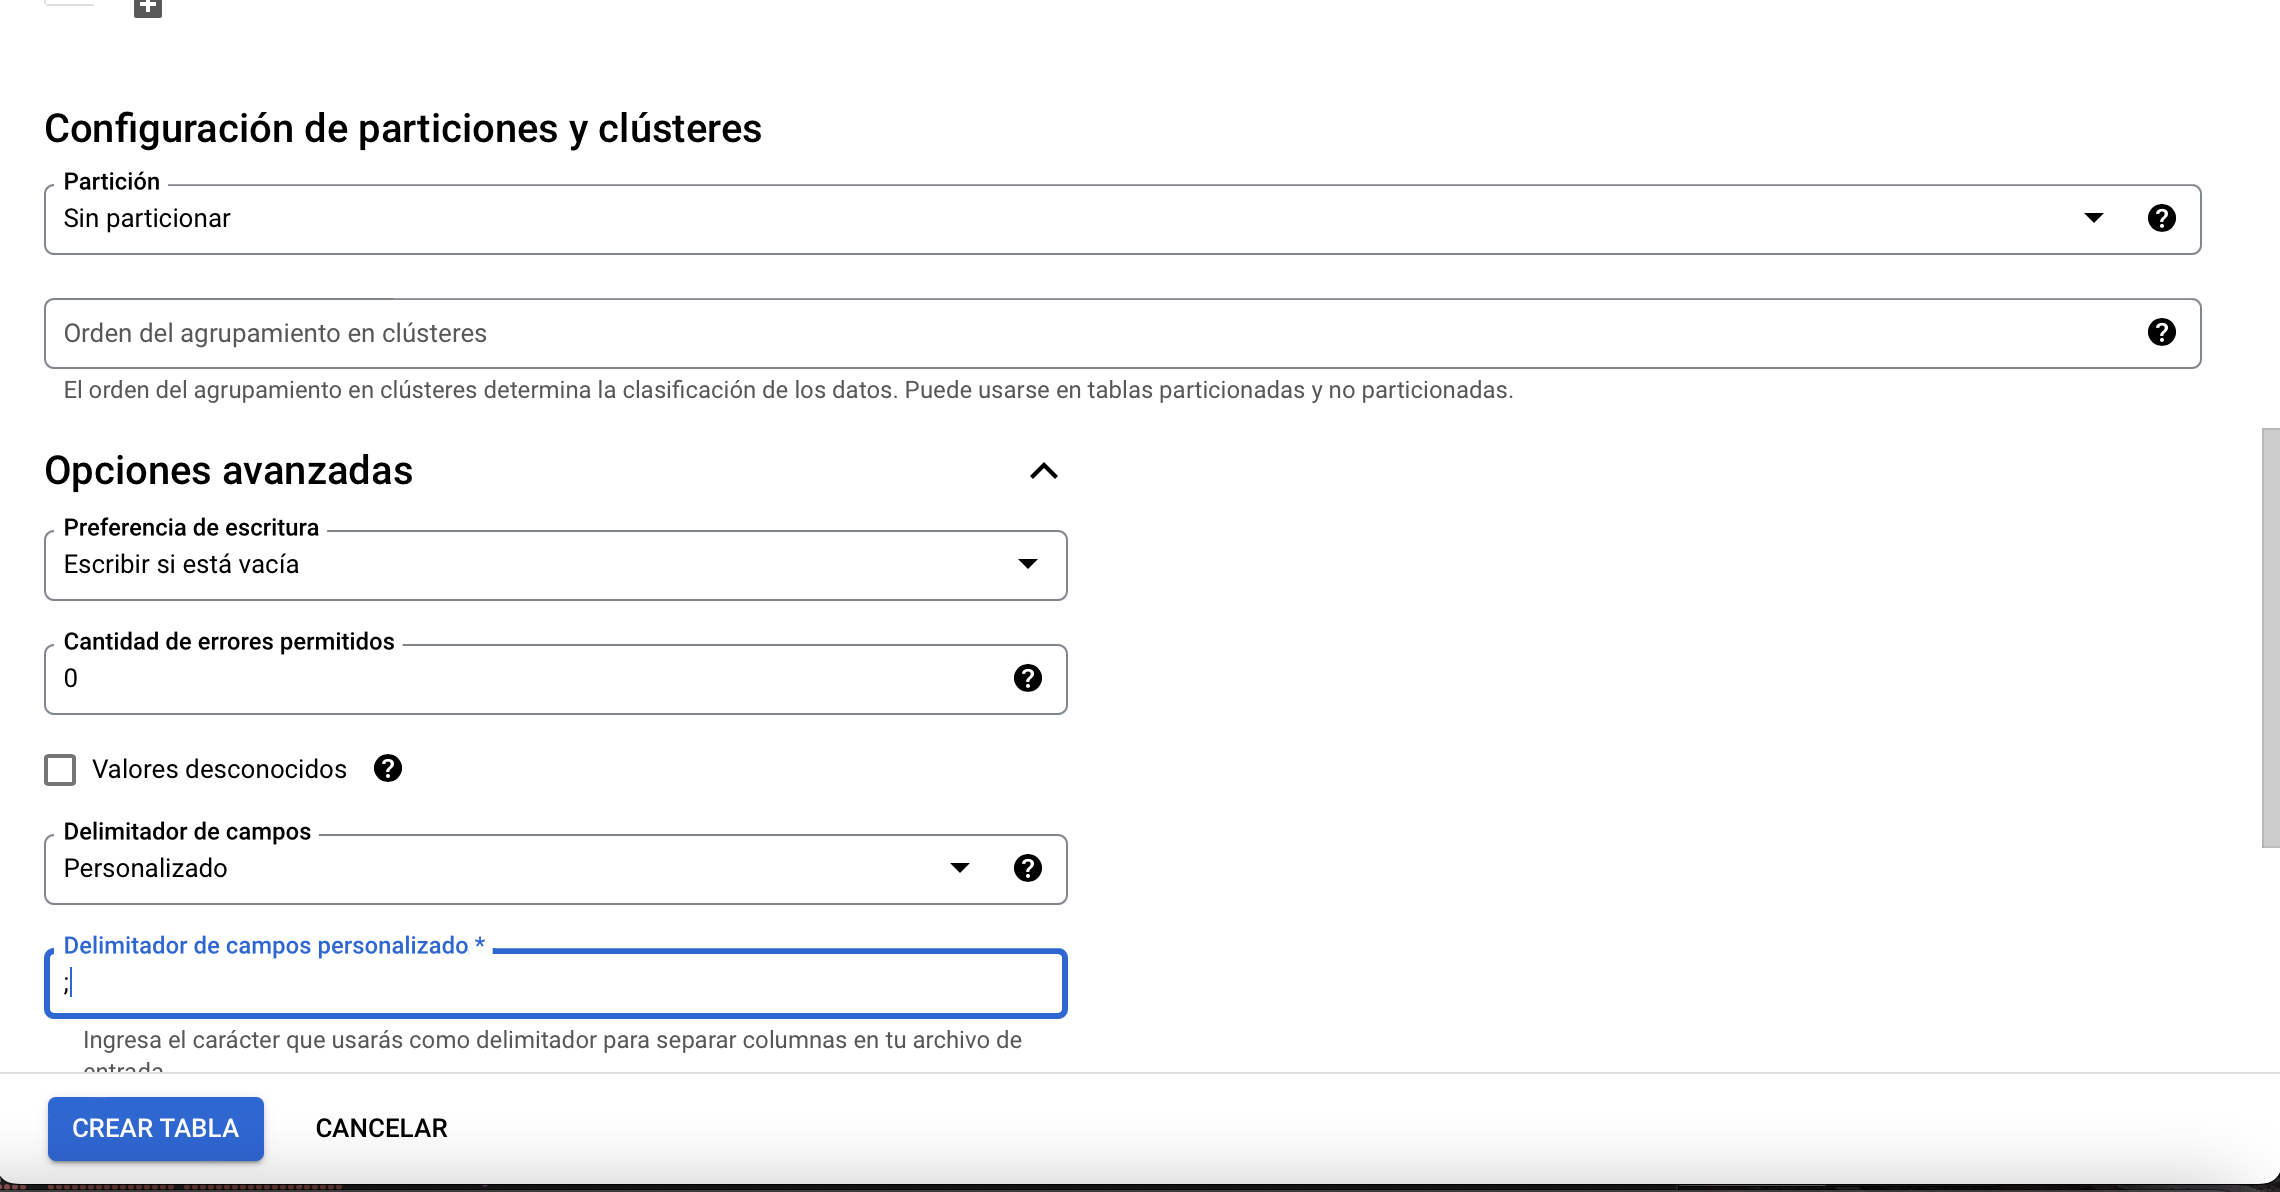
\includegraphics[width=7.25cm]{bq13}}%
\par

\caption{Lectura d'un arxiu extern}
\label{fig:bq12}
\end{figure}


Quant al projecte i al conjunt de dades, els deixarem com estan. I escollirem el nom de la taula, \verb|accidents_bd|, el qual farà saber que inclou informació sobre diversos accidents de trànsit. A continuació, tenim l'opció de definir explícitament l'esquema. això no obstant, atès que es tracta d'un arxiu CSV amb múltiples columnes, podem triar l'opció de detectar automàticament. D'aquesta manera, BigQuery donarà un cop d'ull al contingut de cada columna i determinarà quin ha de ser l'esquema. 



Més enllà d'això, al final de la finestra de creació de la taula ens apareixeran unes opcions avançades. Aquestes opcions permeten la lectura de diferents tipus de CSV, entre altres coses. Sabem que el delimitador de camps d’un CSV pot ser una tabulació o una coma entre altres possibilitats. En el nostre cas, cal especificar que el nostre tabulador és el punt i coma “;”. 



Si hem establert totes aquestes especificacions, ja podrem començar amb l’anàlisi.



Ara es pot comprovar que \verb|accidents_bd| apareix dins la nostra base de dades, \verb|dades_projecte|. A continuació, podem accedir a la informació de la taula i al seu contingut desplegant el menú i triant \texttt{Obrir}. En l'esquema de la taula, sortirà que s'ha detectat automàticament el tipus dels diferents camps. Donem un cop d'ull als detalls de la taula. Aquí es pot veure que la grandària total és de poc més de 280 kB. El nombre de files és d'unes 2.780. I després, quan ens dirigim a la vista prèvia, obtenim un cop d'ull als continguts (Figura ~\ref{fig:bq13}). 


\begin{figure}[h!]
\par
\raisebox{-.5\height}{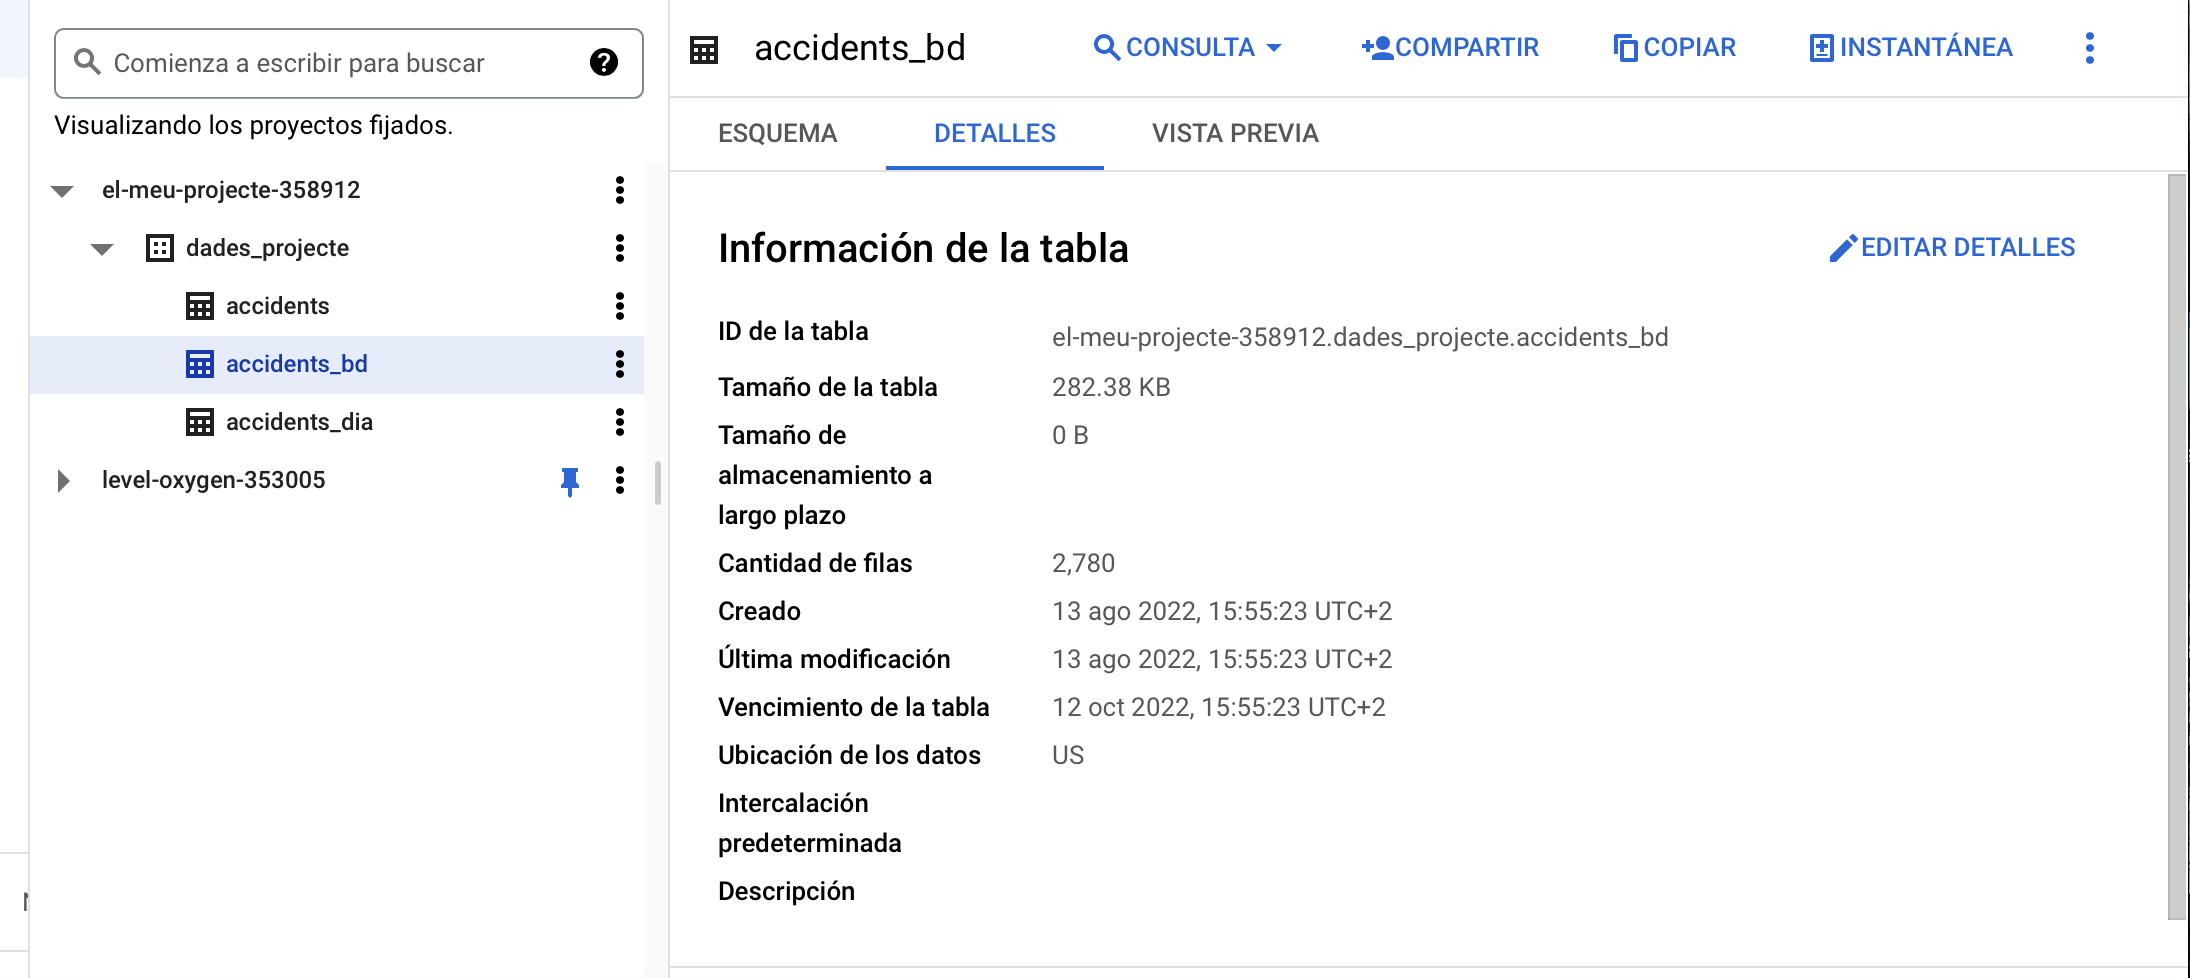
\includegraphics[width=7.25cm]{bq13_2}}%
\hfill
\raisebox{-.5\height}{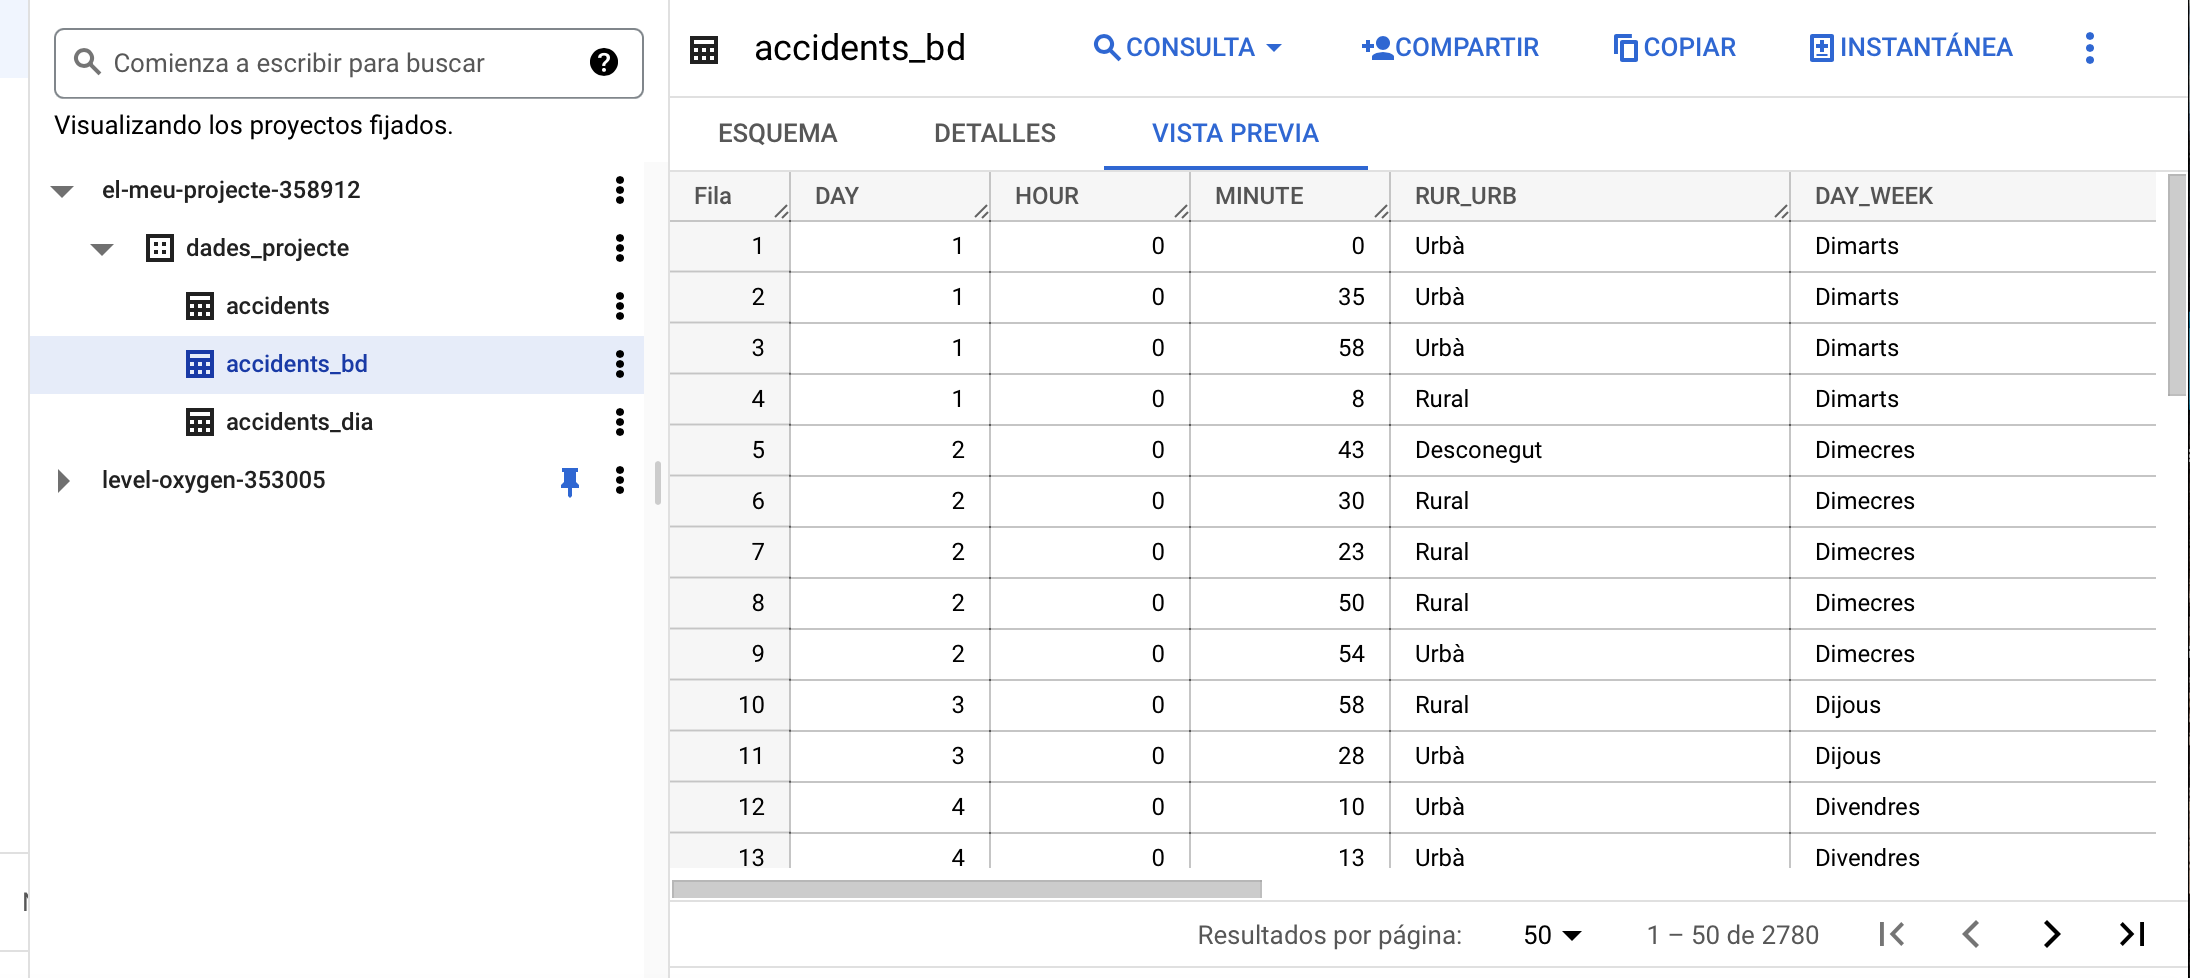
\includegraphics[width=7.25cm]{bq13_3}}%
\par

\caption{Informació sobre la taula}
\label{fig:bq13}
\end{figure}



\subsection{Consulta de dades i visualització d'estadístiques de consultes}

Per a executar consultes en aquesta taula, ens dirigim al botó de consulta i s'obrirà en una nova pestanya. Aquesta pot ser una pestanya completament nova, és a dir, ocultant aquesta vista de detalls, o bé pot ser una pestanya dividida, que ens permetrà veure alhora aquesta vista de detalls per a la taula mentre construïm una consulta. Mitjançant aquest procés, ha aparegut una nova pestanya cap a la dreta, i la consulta que apareix per defecte inclou una clàusula \verb|SELECT|, però no inclou cap camp (Figura ~\ref{fig:bq14}). Precisament per això hi ha un error de sintaxi, com es mostra a la dreta de la figura. 


\begin{figure}[h!]
\par
\raisebox{-.5\height}{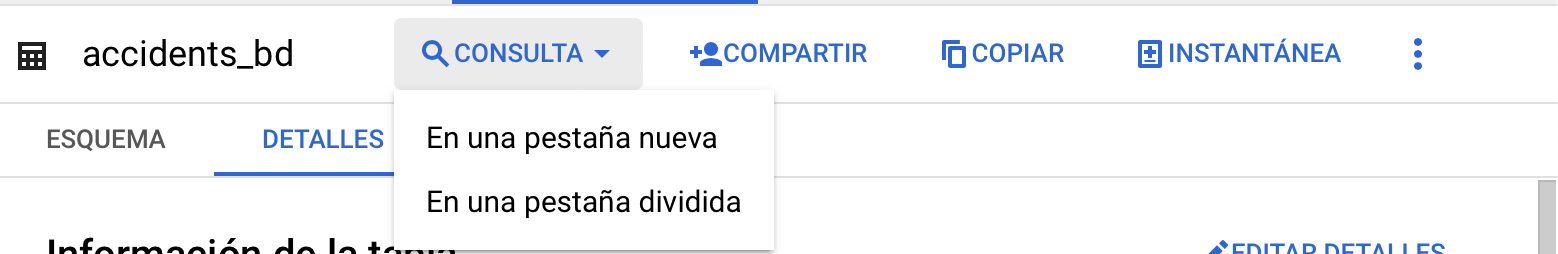
\includegraphics[width=7.25cm]{bq14}}%
\hfill
\raisebox{-.5\height}{
\includegraphics[width=7.25cm]{bq15}}%
\par

\caption{Elaboració d'una consulta}
\label{fig:bq14}
\end{figure}


Ara, per a completar la clàusula \verb|SELECT|, podríem escriure els noms dels atributs que volem consultar, a més de condicions, per exemple, mitjançant la clàusula \verb|WHERE|. Concretament, l'esquema que s'haurà de seguir per a consultar la base de dades té la forma següent:


\begin{verbatim}
SELECT atribut1, atribut2,...
FROM `[nom_projecte].[nom_base_de_dades].[nom_taula]`
(WHERE condició)
\end{verbatim}



Si escrivim a l’editor la nostra consulta, apareixerà un validador d’aquesta a la part superior dreta de la finestra. Aquest validador l'hem vist anteriorment quan ens indicava un error en voler executar una consulta fent servir llenguatge de manipulació de dades (DML), i pot agafar dues formes:

- Si la consulta és vàlida, apareixerà una icona de verificació en color verd.

- Si la consulta no és vàlida, apareixerà una icona d’exclamació en color vermell

A més, el validador també mostra la quantitat de dades que la consulta processarà quan s’executi. Per exemple, si demanem en una consulta que ens retorni la columna sencera \verb|DAY|, el validador de la dreta ens marca que es processaran una quantitat de gairebé 22 kB, tal com es pot veure a la figura ~\ref{fig:bq19}.


\begin{figure}[h!]
\begin{center}
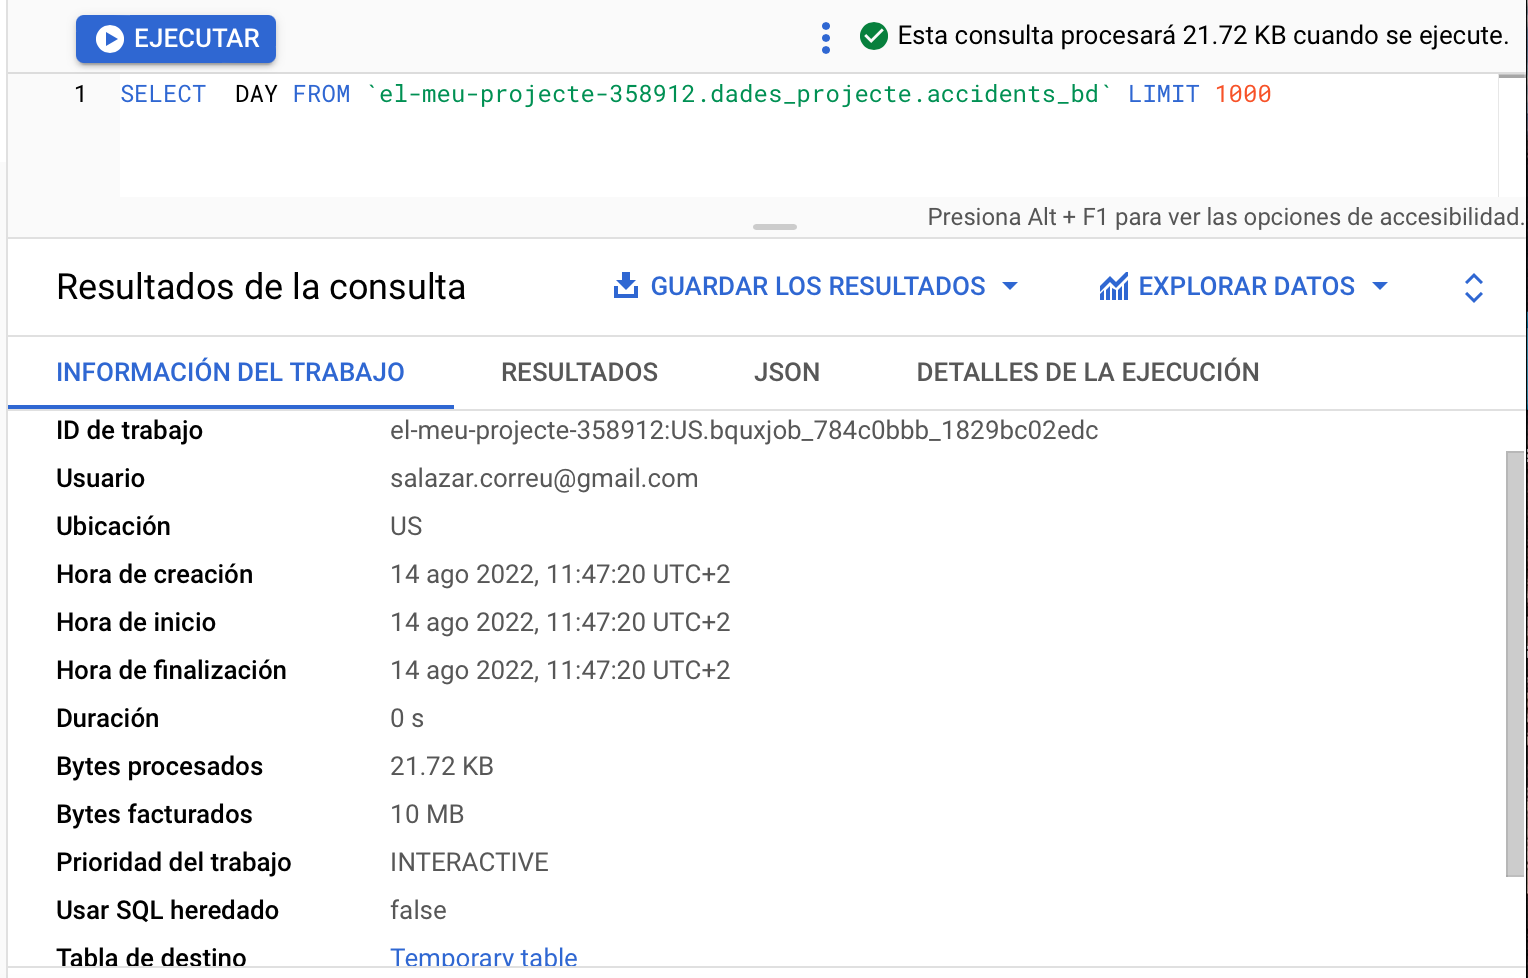
\includegraphics[width=10cm]{bq19}
\end{center}
\caption{Primera consulta}
\label{fig:bq19}
\end{figure}


Efecturem aquesta consulta prement \textit{Ejecutar}. Els resultats apareixen sota la finestra d'editor i mostra certs detalls com, per exemple, que la consulta s'ha executat en uns 0 segons. Per descomptat, podem desplaçar-nos i donar un cop d'ull a tots els resultats (a la dreta de la Figura ~\ref{fig:bq19}). Entre els detalls que es mostren per a cada consulta s'hi troben la informació del treball, els resultats en forma de taula, els resultats en format JSON i certs detalls de l'execució de la consulta. 



Si posem el focus en la informació del treball, es troba l'identificador d'aquest, l'usuari que l'ha executat, la ubicació on s'emmagatzemen les dades, l'hora de la creació i l'execució d'aquesta, el temps d'execució i els bytes processats i facturats. Veiem que el nombre de bytes facturats és de 10 MB, aquesta és la quantitat mínima que surt per defecte per a cada consulta per \textit{Google Cloud Platform}, i té en compte les despeses generals. Per a consultes a bases de dades més extenses, aquesta facturació serà major i ens impedirà l'ús de la zona de proves. L'última característica que crida l'atenció de la informació del treball és que els resultats s'emmagatzemen en una taula temporal. Això vol dir que aquesta taula resultant no es guardarà com una més en el nostre conjunt de dades i, per tant, no la podrem consultar.



\subsection{Creació d'una taula a partir d'un resultat de consulta}

Una altra alternativa a les taules temporals serà crear una taula en el nostre conjunt de dades a partir d'una taula temporal o vista. En aquest cas, farem una sèrie temporal de 31 observacions que ens compti el nombre d'accidents ocorreguts cada dia del mes a partir de la consulta següent:

\begin{verbatim}
SELECT DAY, COUNT(*) AS FREQ
FROM `el-meu-projecte-358912.dades_projecte.accidents_bd`
GROUP BY DAY
\end{verbatim}

Un cop realitzada la consulta, hem d'exportar totes aquestes dades a una nova taula i, per a fer-ho, revisarem algunes de les opcions d'exportació que es troben al menú \textit{Guardar resultados}. En aquest, apareixen diverses opcions per a la manera de guardar els resultats (Figura ~\ref{fig:bq17}). Podem guardar-los com un arxiu CSV en Google Drive o en un arxiu local. En el nostre cas, exportarem el contingut a una nova taula de BigQuery. Una vegada feta aquesta selecció, podem decidir el nom del projecte i el conjunt de dades on s'aprovisionarà la taula i, a més, establir un nom de taula. 


\begin{figure}[h!]
\par
\raisebox{-.5\height}{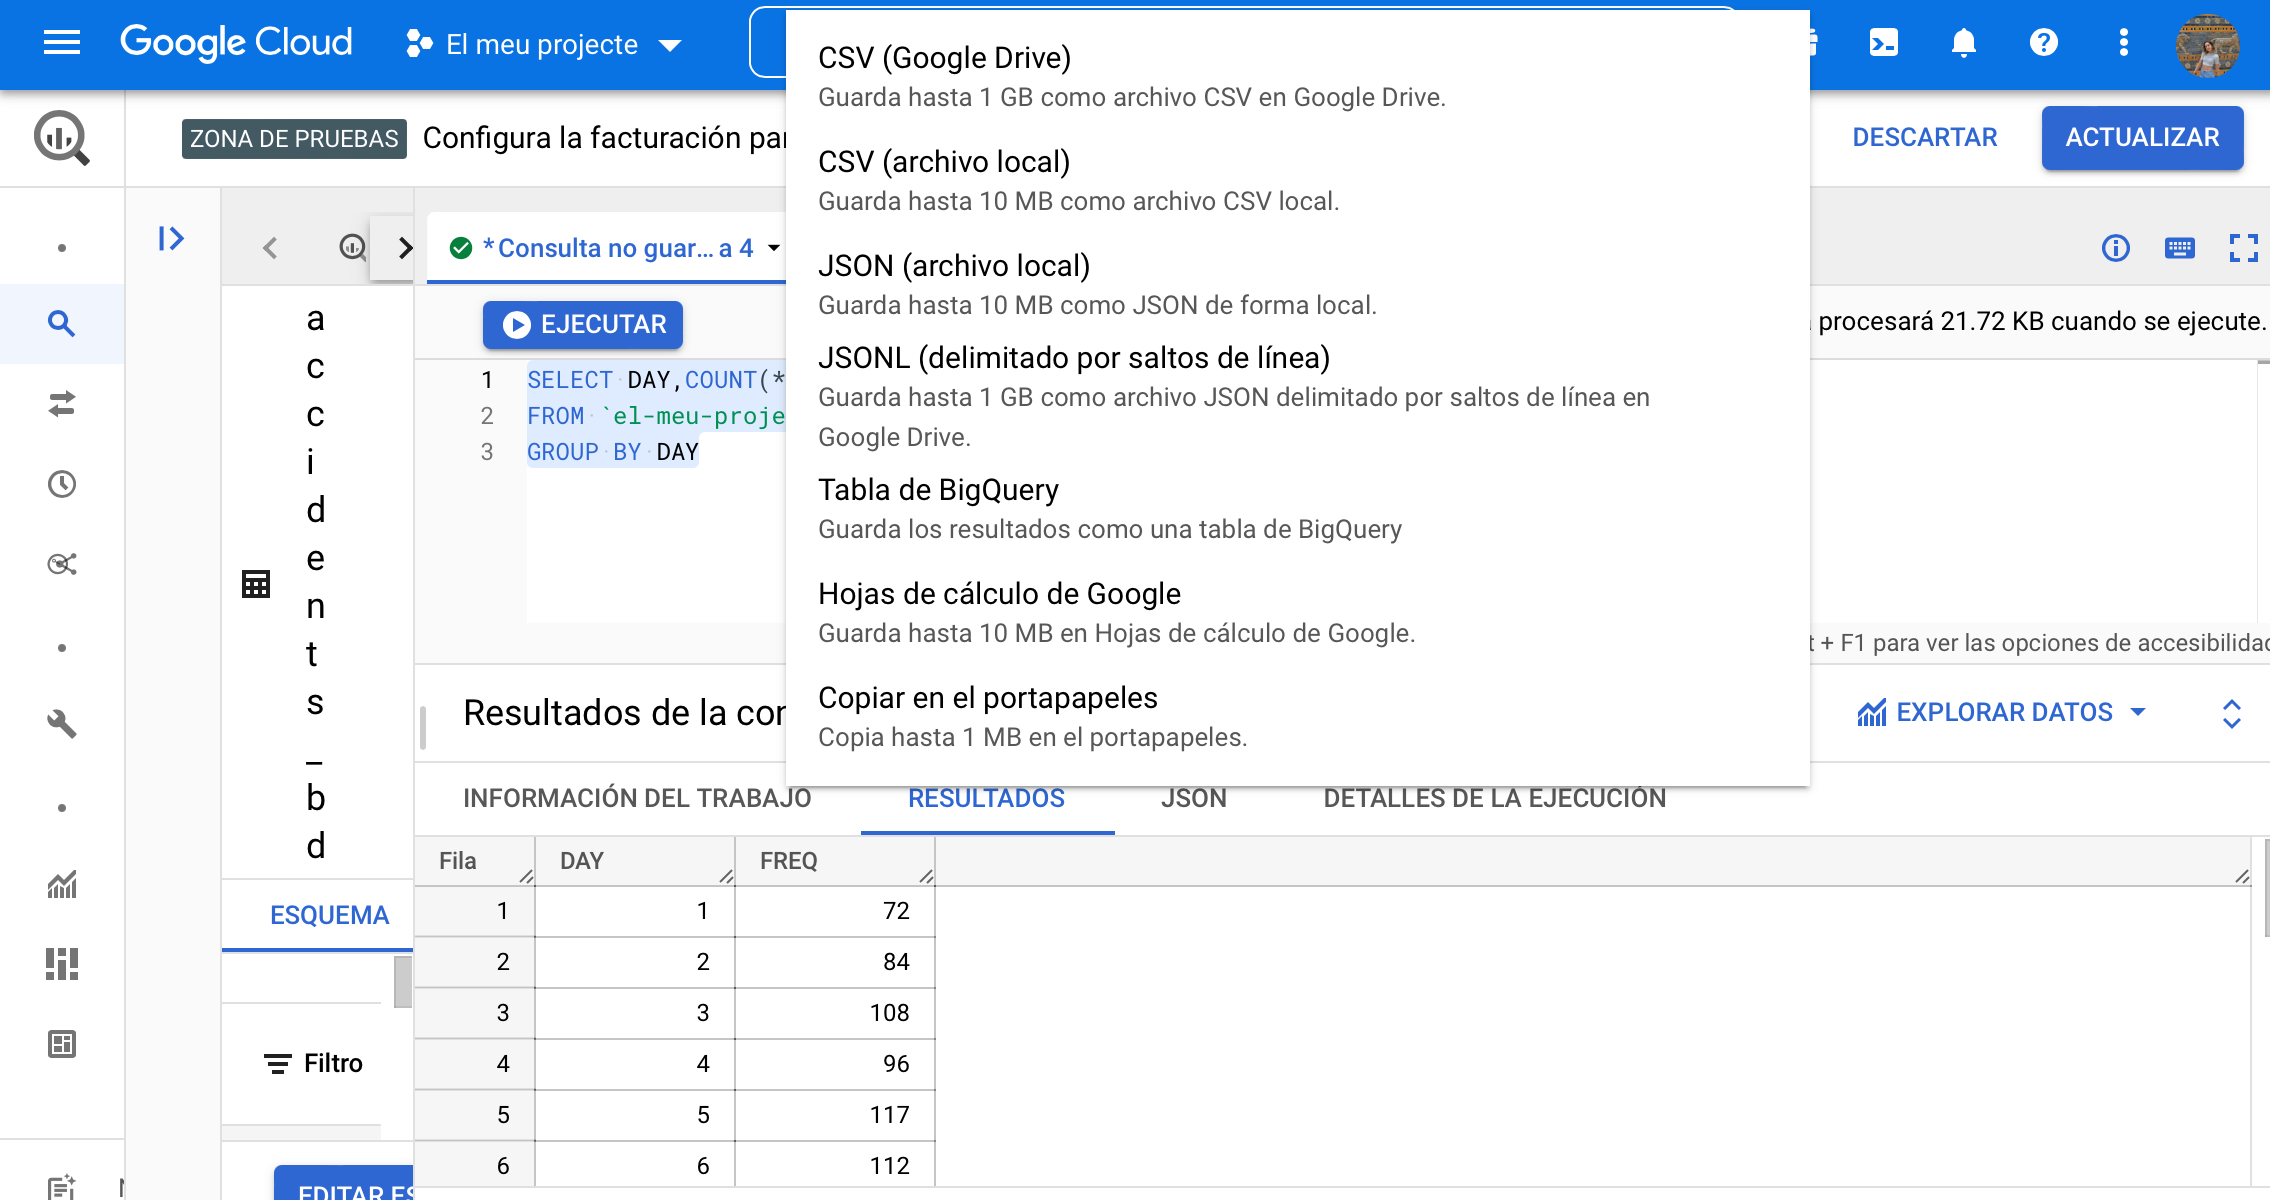
\includegraphics[width=7.25cm]{bq17}}%
\hfill
\raisebox{-.5\height}{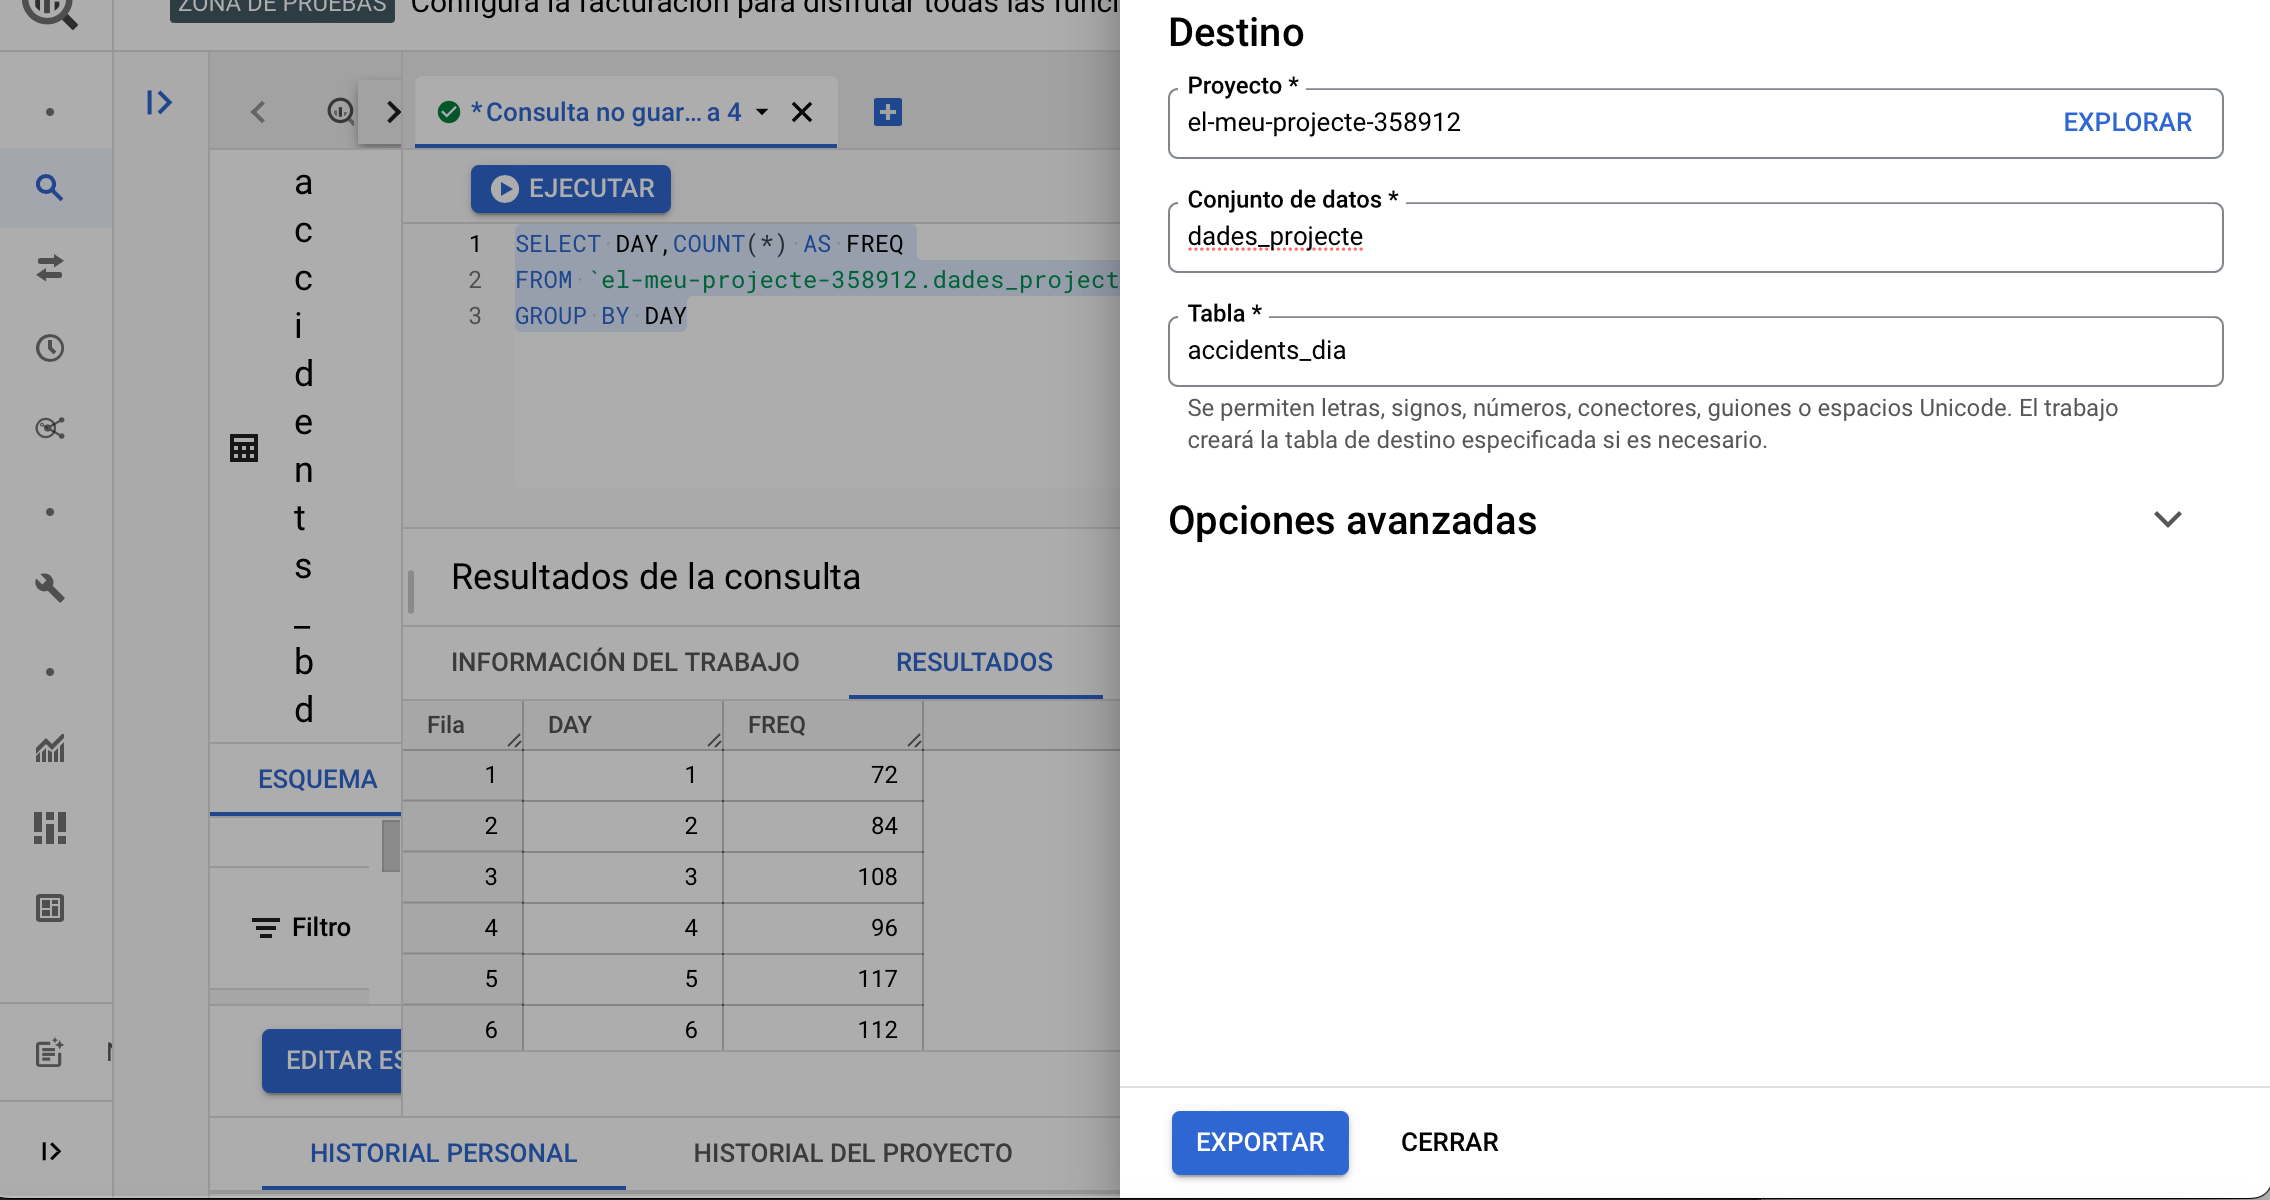
\includegraphics[width=7.25cm]{bq18}}%
\par

\caption{Creació d'una taula a partir d'una consulta}
\label{fig:bq17}
\end{figure}



Llavors, quan guardem les coses, això haurà iniciat un nou treball per a guardar la nova taula i carregar-la amb dades. Una vegada que tanquem aquesta notificació, podem treure el pin de l'Explorador i, avall, hi apareix com una taula. En obrir-la confirmem que l'esquema apunta a les mateixes columnes que havíem referenciat en la clàusula \verb|SELECT| de la consulta que va crear aquesta taula. Des dels detalls podem confirmar que el nombre de files coincideix amb el dels resultats de la consulta, concretament 31. I després la vista prèvia ens mostrarà quines són les dades exactament. 



Hom es pot preguntar: \textit{Quina és la finalitat d'aquesta taula?} Bé, atès que només conté un subconjunt de la taula original, les consultes cap a aquesta taula tindran potencialment menys dades per a processar que les consultes que s'executen directament a la taula original. Potser en aquest cas no tornarem a necessitar aquesta consulta, però imaginem que només ens interessa estudiar els accidents que s'hagin produït a zones rurals i creem una consulta que filtri aquest tipus de casos. En aquesta situació, serà millor executar la resta de consultes sobre la taula petita, que inclou tota la informació que necessitem i probablement tindrà un cost de consulta menor.

\newpage

\section{Dades públiques i dades externes}

\subsection{Conjunts de dades públiques a BigQuery}

Mentre continuem familiaritzant-nos amb la plataforma, podem explorar una altra opció que ofereix BigQuery, que són dades que estan disponibles públicament per a que qualsevol usuari pugui executar les seves consultes. Aquests conjunts de dades públiques es troben en un projecte anomenat \textit{BigQuery Public Data}. Per a accedir a elles, farem servir al botó d'agregació de dades (\verb|ADD DATA|) que es troba al costat de l'explorador, i escollirem l'opció \textit{Explorar conjuntos de datos públicos}) (Figura ~\ref{fig:bq20}).


\begin{figure}[h!]
\begin{center}
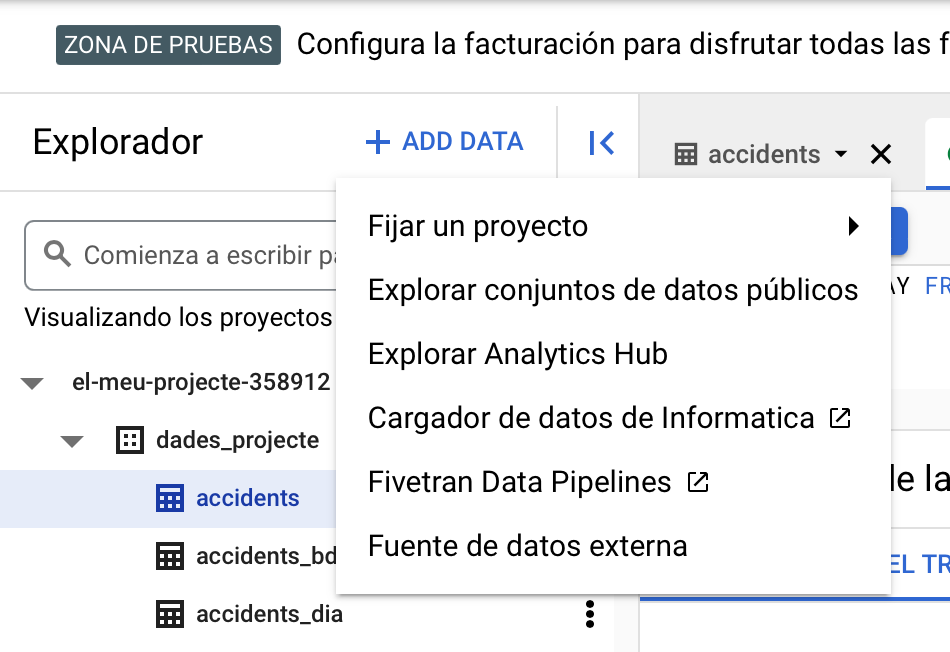
\includegraphics[width=10cm]{bq20}
\end{center}
\caption{Accés als conjunts de dades públiques}
\label{fig:bq20}
\end{figure}


Podem donar un cop d'ull als diferents conjunts de dades i taules d'aquest projecte i navegar entre les diferents opcions per a poder triar aquells que cridin la nostra atenció i, en definitiva, amb els que treballarem. Per exemple, entre totes aquestes taules s'hi troba una que conté informació sobre la població catalana recopilada per l'aplicació \textit{GenCat Mobile Coverage} (Figura ~\ref{fig:bq21}). Dins d'aquesta taula s'hi troben dades recollides mitjançant crowdsourcing\footnote[1]{La pràctica d'obtenir informació o aportacions a una tasca o projecte recorrent als serveis d'un gran nombre de persones, remunerades o no, normalment a través d'Internet.} i tenen informació sobre l'estat de la cobertura de la telefonia mòbil a Catalunya. La plataforma utilitza una aplicació Android per a registrar les dades dels ciutadans a través dels seus dispositius mòbils sobre el nivell de cobertura per operador, la xarxa utilitzada (2G, 3G i 4G) i la ubicació del dispositiu. Aquestes dades en concret van ser recopilades durant els anys 2015-2017.




\begin{figure}[h!]
\par
\raisebox{-.5\height}{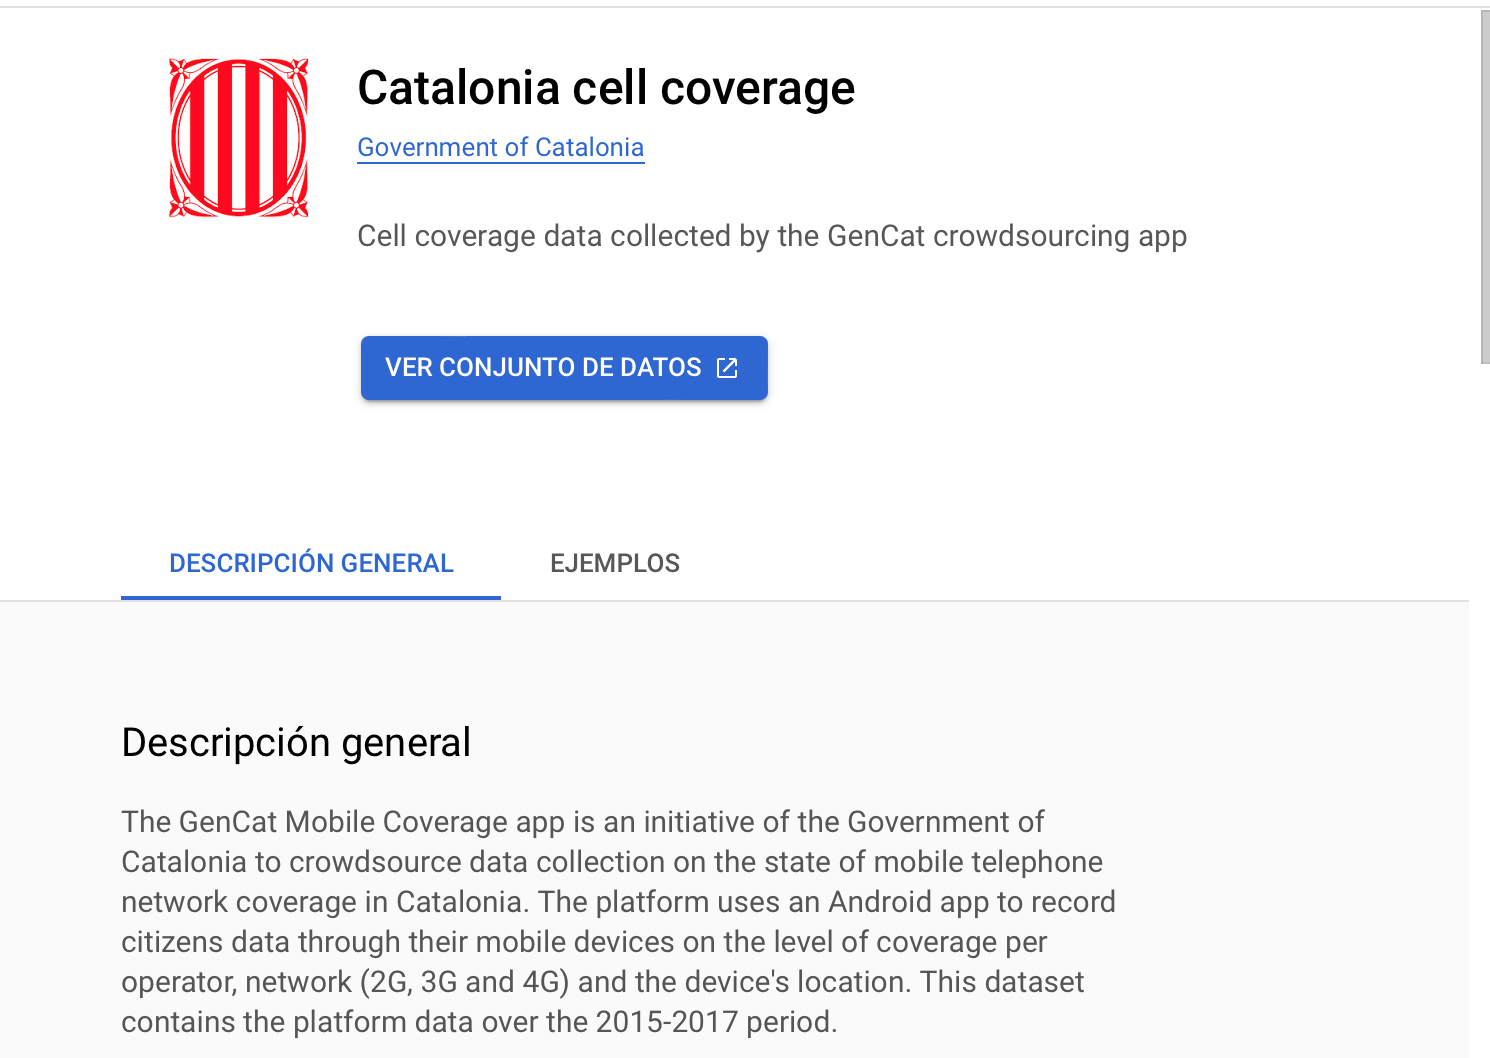
\includegraphics[width=7.25cm]{bq21}}%
\hfill
\raisebox{-.5\height}{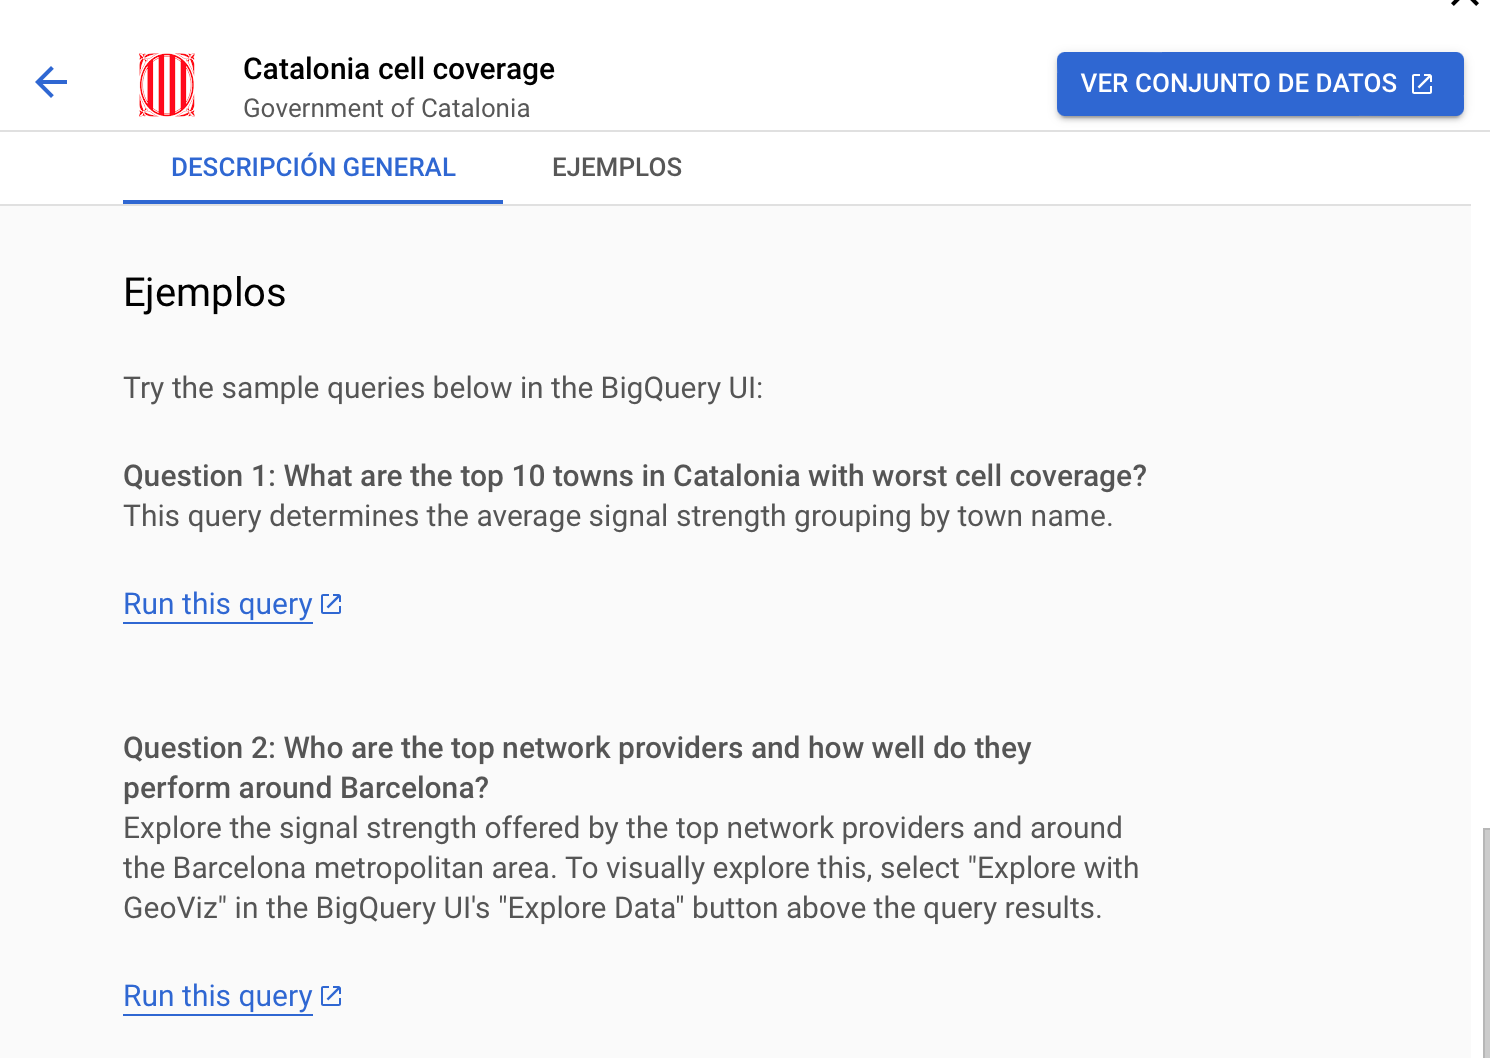
\includegraphics[width=7.25cm]{bq22}}%
\par

\caption{Creació d'una taula a partir d'una consulta}
\label{fig:bq21}
\end{figure}


Si volguéssim descarregar la taula i situar-la dins del nostre projecte, BigQuery ens permet aquesta operació si premem \textit{Ver conjunto de datos} seguit de \textit{crear tabla}. Això no obstant, també és possible consultar la taula sense necessitat de descarregar-la dins del nostre projecte, fent servir el projecte \verb|bigquey-public-data|, que és el que farem en aquest cas.



Dins la informació de la taula que ens proporciona la plataforma, apareix una secció amb consultes suggerides (les podem trobar a la dreta de la Figura ~\ref{fig:bq21}). D'entre aquestes, la primera fa referència als 10 pobles catalans amb pitjor cobertura de mòbil.  Si premem el botó \textit{Run this query}, el navegador ens redirigeix a l'editor amb la consulta preparada, i nosaltres la podem executar sense cap cost, ja que tant la taula com el resultat de la consulta estan emmagatzemats a BigQuery i les dades no s'han de processar (Figura ~\ref{fig:bq23}).


\begin{figure}[h!]
\begin{center}
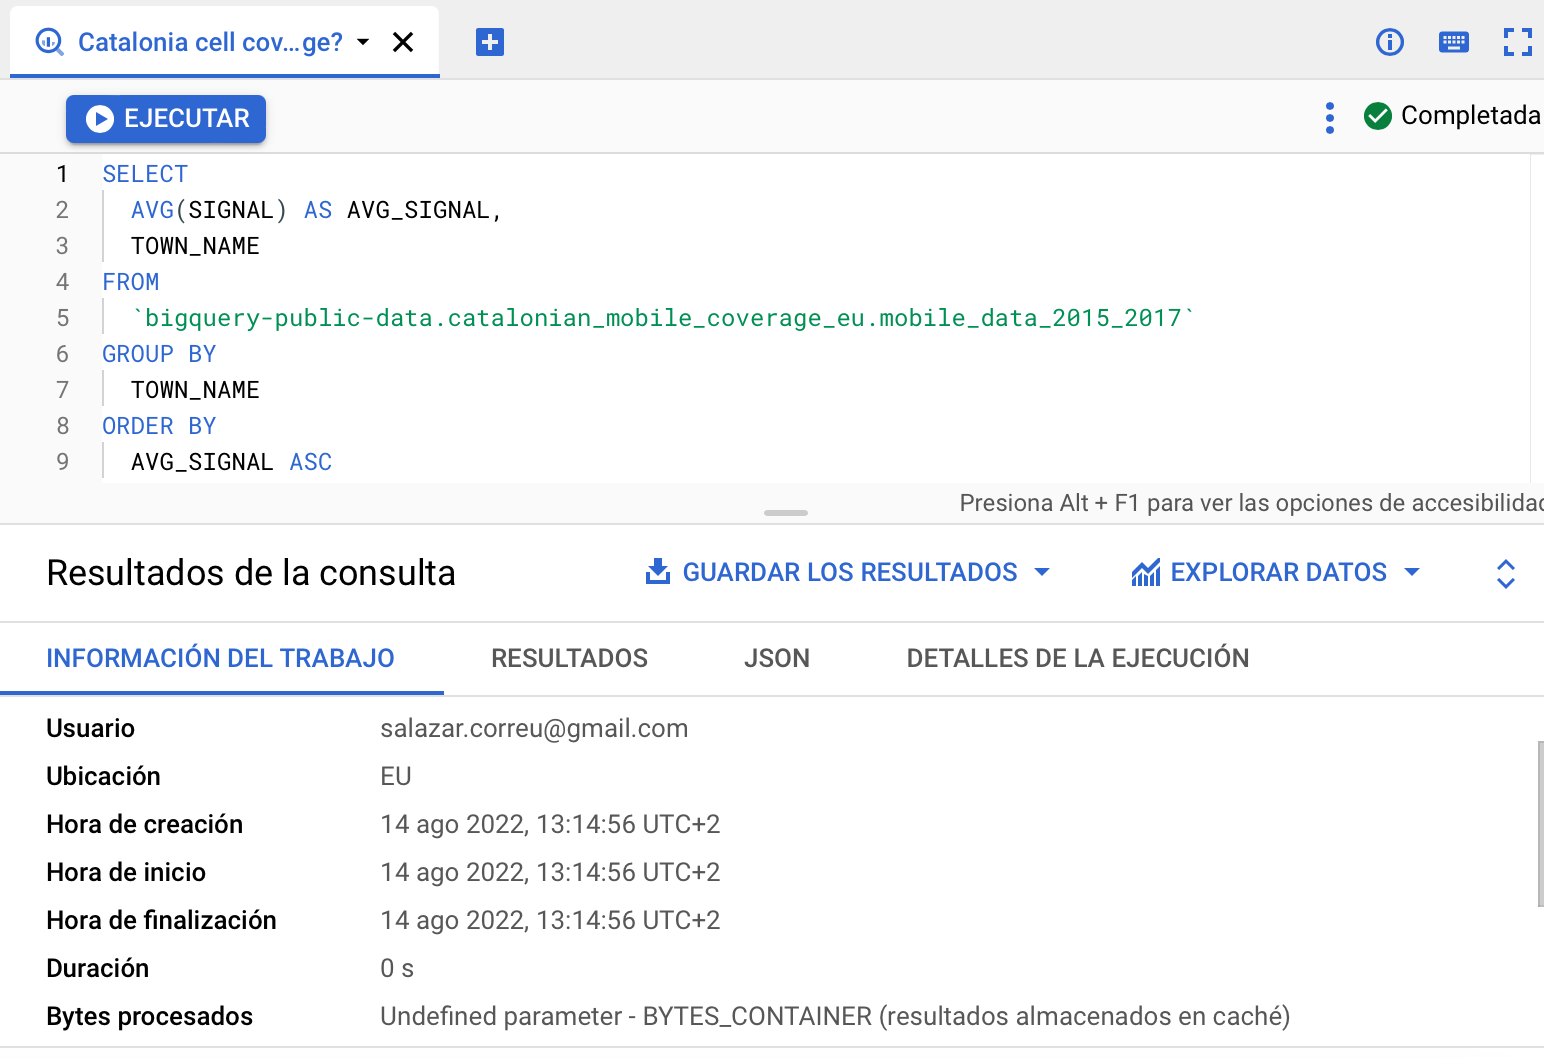
\includegraphics[width=10cm]{bq23}
\end{center}
\caption{Consulta a un conjunt de dades públic}
\label{fig:bq23}
\end{figure}


Els resultats d'aquesta consulta ens diuen que els pobles catalans amb menys cobertura mòbil són Canejan, Boadella i les Escaules, Cabó, la Vajol, Gaià, Farrera, Gisclareny, Viver i Serrateix, Savallà del Comtat i Torroja del Priorat. A més, els bytes processats en aquesta consulta apareixen com un paràmetre indefinit, ja que aquests resultats estan emmagatzemats a la memòria cau de BigQuery.



Tal com hem vist, BigQuery emmagatzema a la seva memòria cau els resultats de la consulta perquè les dades puguin ser recuperades més ràpidament la pròxima vegada que s'executi una mateixa consulta. Això no obstant, cal tenir en compte que només s'accedeix a les dades de la memòria cau quan s'executa la mateixa consulta després de la seva creació. Per exemple, si es modifiqués una mica aquesta consulta i demanés tan sols el nom del poble, en comptes d'aquest i la mitjana del senyal mòbil, podríem arribar a pensar que els resultats de la consulta d'aquesta execució haurien de retornar-nos un subconjunt de les dades que ja són presents en la memòria cau (ja que és un subconjunt de la nostra consulta anterior). Però, per la forma en què funciona la memòria cau de BigQuery, quan executem això, observarem que la informació no s'ha recuperat d'aquesta. En canvi, quan aquesta consulta es torna a executar, és quan la memòria cau s'activa, i és d'on es recuperen les dades. 



Per tant, la memòria cau només funciona si és la mateixa consulta la que es torna a executar. Aquestes característiques són de gran interès, ja que l'emmagatzematge en memòria cau és una gran manera de reduir el cost d'execució de les consultes, i també millora el rendiment d'aquestes. 

\subsection{Taules externes de BigQuery}

Una altra funció que presenta la plataforma és la lectura d'arxius externs que s'actualitzen de forma periòdica. Això és d'especial utilitat en els casos en què la informació de la qual es disposa és a temps real, que és una característica prou habitual quan es treballa amb volums de dades molt elevats. Per a il·lustrar el funcionament de BigQuery en aquests casos, crearem una nova taula que estarà vinculada, en aquest cas, a Google Drive, concretament als fulls de càlcul de la plataforma (Figura ~\ref{fig:bq24}). És molt important que el propietari de la taula sigui el mateix compte que està vinculat a BigQuery, perquè en cas contrari sorgeix un missatge d'error i no és capaç de vincular la taula externa.


\begin{figure}[h!]
\begin{center}
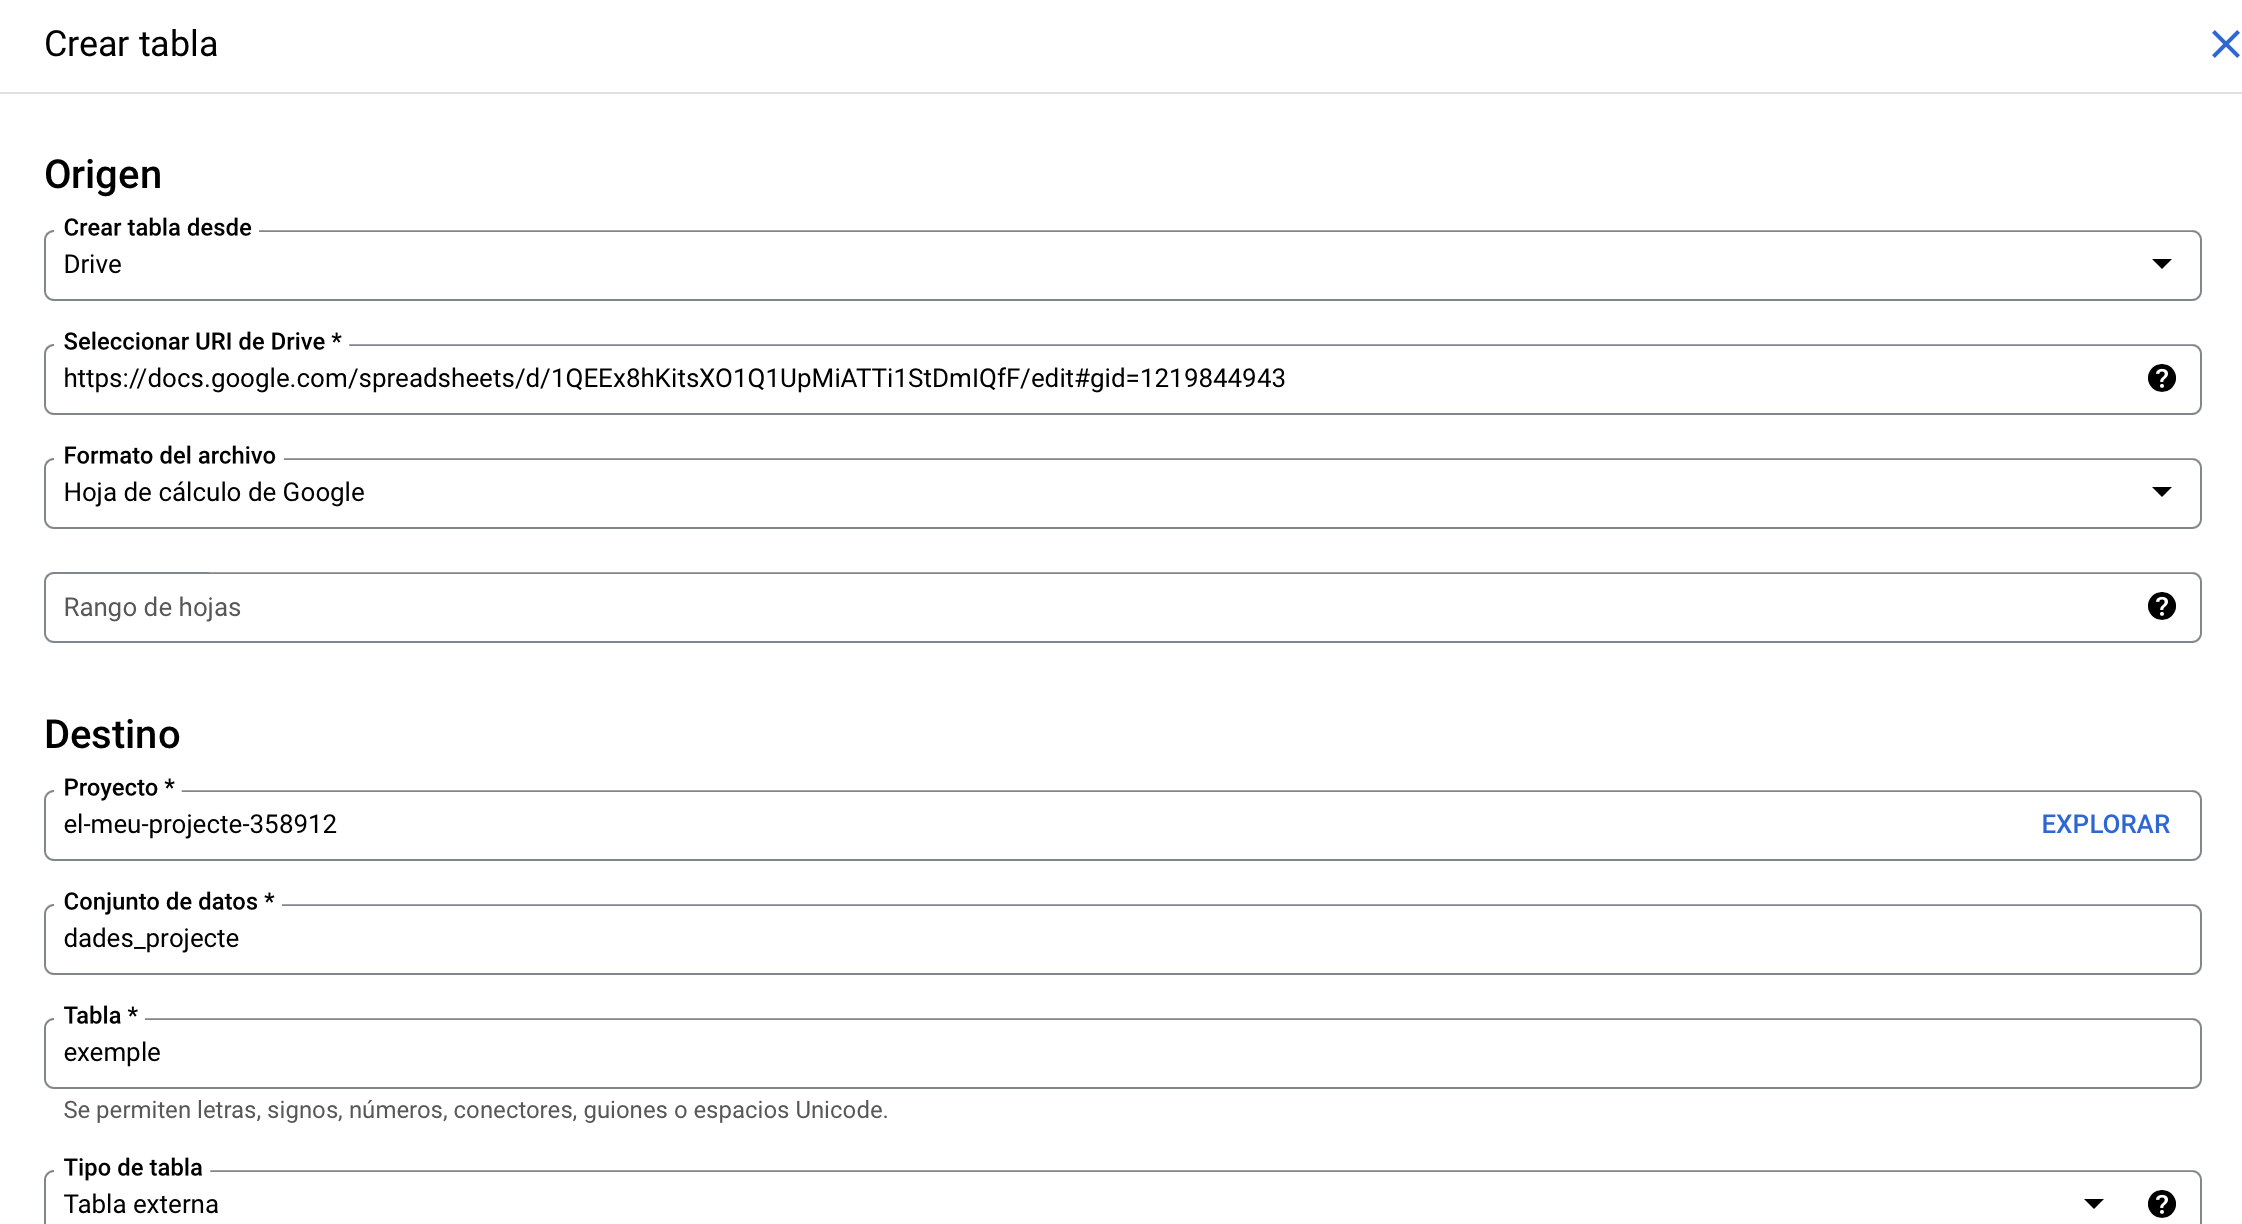
\includegraphics[width=10cm]{bq24}
\end{center}
\caption{Connexió a una taula externa}
\label{fig:bq24}
\end{figure}



Si ens dirigim als detalls, aquí és on veiem quelcom interessant. La grandària de la taula és de zero bytes, atès que les dades són externes a BigQuery (Figura ~\ref{fig:bq25}). Si ens desplacem, podem veure els detalls de les dades externes. Això significa que quan actualitzem el full de càlcul, qualsevol consulta cap a aquesta taula recollirà automàticament les dades més recents. Ja que la nostra consulta de la taula gran no és només una còpia del full de càlcul, sinó que és de fet una referència a ella. Parlant de consultar les dades, ens dirigirem a \textit{Query}, i a obrir un editor de consultes en una nova pestanya. Quan una consulta s'executa, totes les dades són retornades a nosaltres, i podem accedir a elles com ho faríem amb qualsevol dada que resideixi en una taula nativa de BigQuery. 


\begin{figure}[h!]
\begin{center}
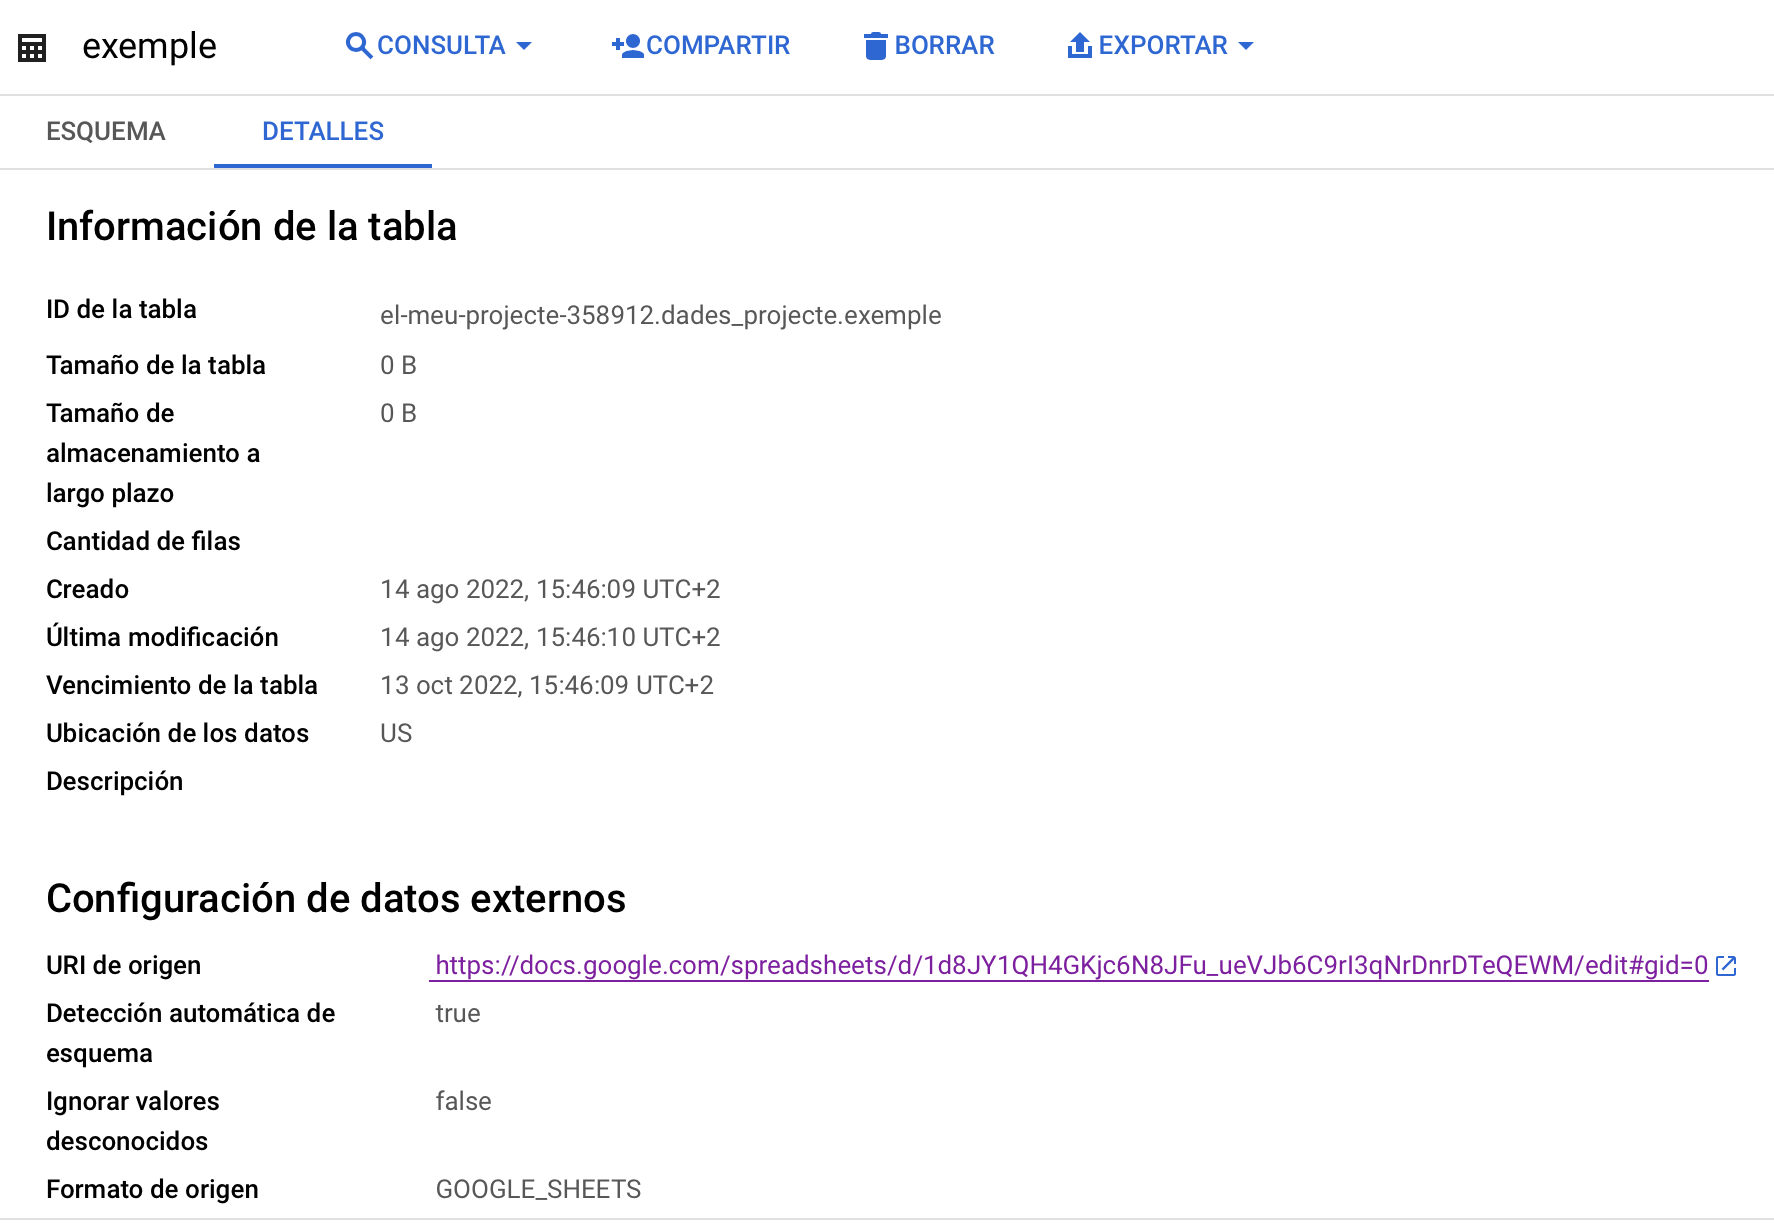
\includegraphics[width=10cm]{bq25}
\end{center}
\caption{Característiques d'una taula externa}
\label{fig:bq25}
\end{figure}


\newpage

\section{Integració de BigQuery amb Looker Studio}

Ara que hem cobert els diferents tipus de taules de BigQuery, ens centrarem en com podem visualitzar les nostres consultes. 


Looker Studio és una eina gratuïta que permet convertir les dades en panells o informes complets, fàcils de llegir, fàcils de compartir i totalment personalitzables. Algunes de les seves funcionalitats són:


- Descriure les dades amb gràfiques, que inclouen gràfics de línies, de barres i circulars, mapes geogràfics, gràfics d’àrea i de bombolles, taules de dades dinàmiques i molt més.


- Permet que els nostres informes siguin interactius amb filtres de visualització.


- Inclou enllaços i imatges en les quals es pot clicar per crear catàlegs de productes, biblioteques de vídeo i altres continguts amb URL.


- Facilita l’anotació i descripció dels informes amb text i imatges.


A més de presentar totes aquestes característiques, amb Looker Studio es poden elaborar fàcilment informes sobre dades procedents d’una gran varietat de fonts, sense necessitat de programar. En tan sols uns instants, ens podem connectar a conjunts de dades com BigQuery.

\subsection{Ús de Looker Studio des de BigQuery}

Imaginem que volem tornar a consultar el nombre d'accidents de trànsit que es van donar cada dia durant aquell mes als Estats Units. Per a fer aquesta consulta, farem servir la \textit{query} anterior:

\begin{verbatim}
SELECT DAY, COUNT(*) AS FREQ
FROM `el-meu-projecte-358912.dades_projecte.accidents_bd`
GROUP BY DAY
\end{verbatim}


\begin{figure}[h!]
\begin{center}
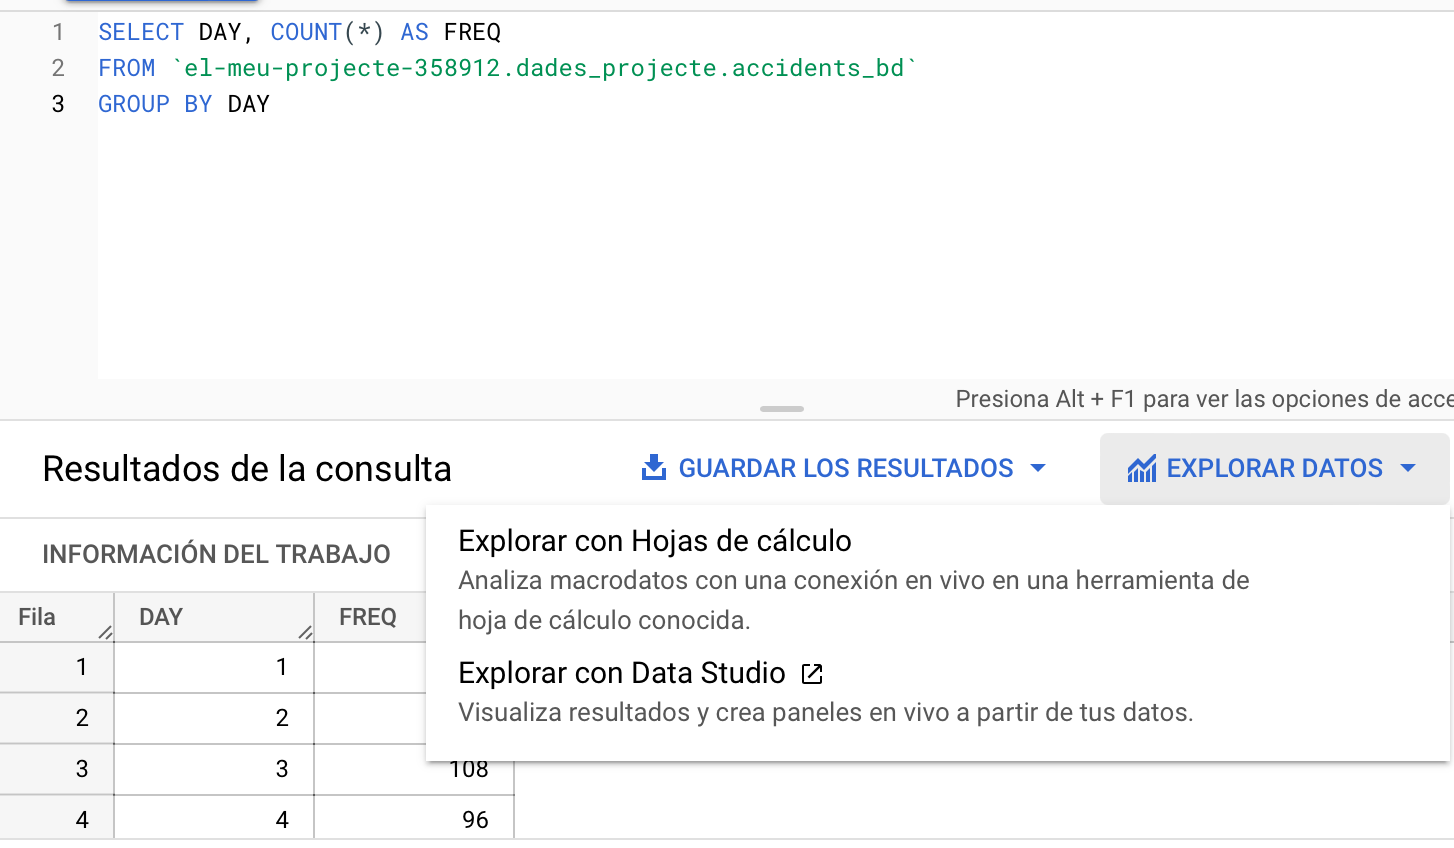
\includegraphics[width=10cm]{bq26}
\end{center}
\caption{Visualització d'una consulta a Looker Studio}
\label{fig:bq26}
\end{figure}


Per a visualitzar la taula resultant, podem ampliar el menú \textit{Explorar datos}, tot seguit d'\textit{Explorar con Looker Studio} (Figura ~\ref{fig:bq26}).


Quan fem aquesta selecció, sorgeix una nova interfície que ja té una taula que conté alguna informació i un histograma amb les dades d'aquesta (Figura ~\ref{fig:bq27}).

\begin{figure}[h!]
\begin{center}
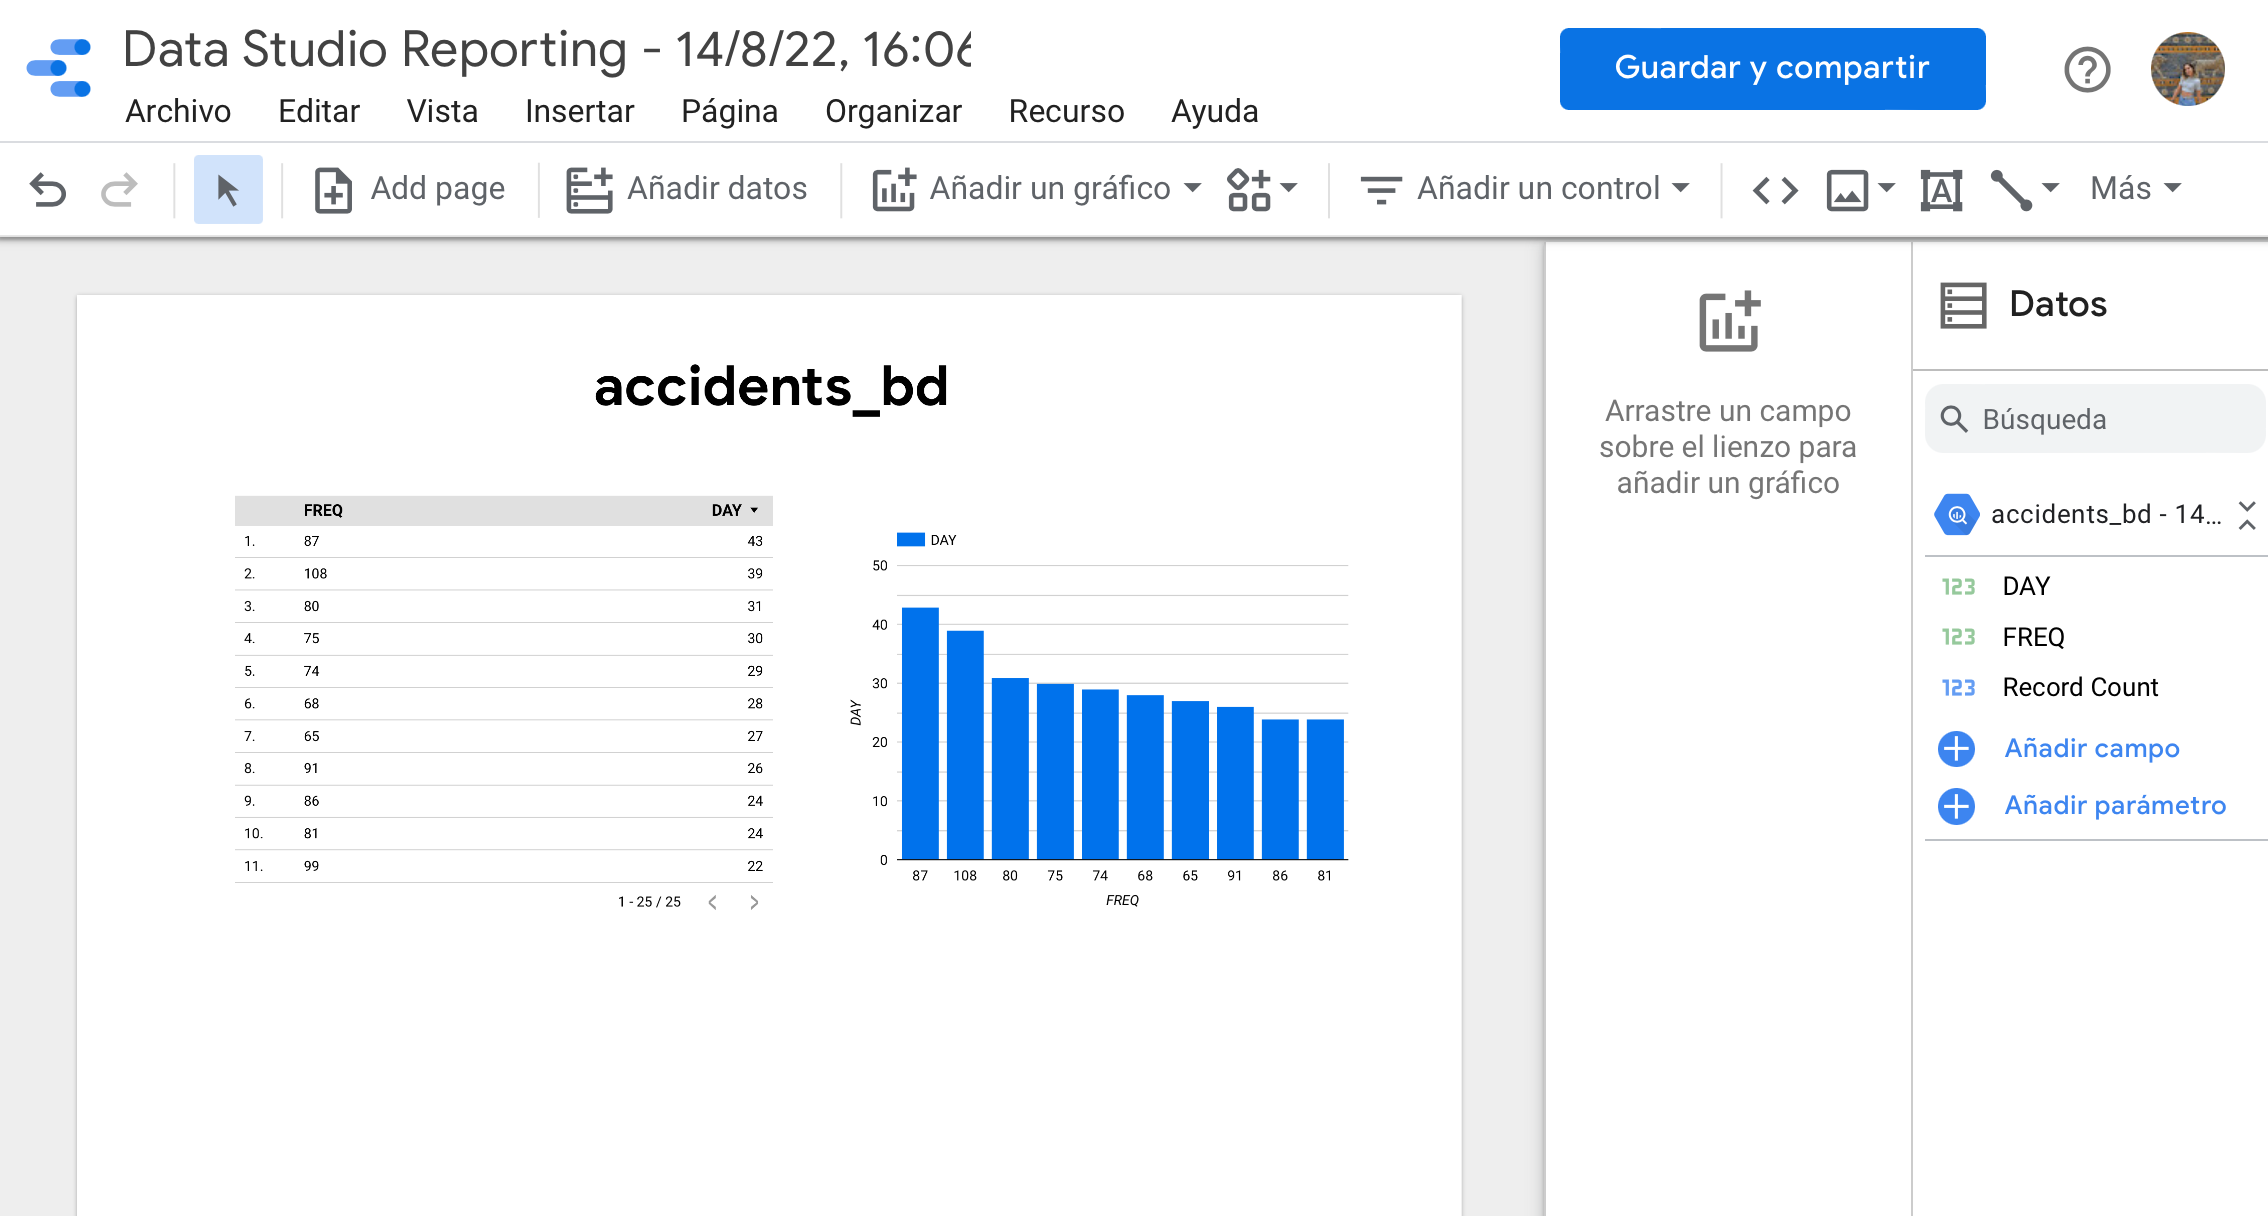
\includegraphics[width=10cm]{bq27}
\end{center}
\caption{Consulta des de Looker Studio}
\label{fig:bq27}
\end{figure}

Data Studio, per defecte, ha entès que una taula de recompte es visualitza normalment a partir d'un gràfic de barres vertical o histograma, i per això l'ha creat sense que nosaltres ho hàgim especificat. Així i tot, nosaltres podem seleccionar una visualització abans de configurar-la per a presentar la informació que necessitem. Pose'm-nos en el cas que preferim un gràfic de barres horitzontal per a la visualització d'aquestes dades. Premem l'opció \textit{Añadir un gráfico} i ens assegurem que la dimensió, que en aquest cas són els dies, i la mètrica, la freqüència dels accidents, estiguin seleccionades segons el que vulguem representar (Figura ~\ref{fig:bq28}). 

\begin{figure}[h!]
\par
\raisebox{-.5\height}{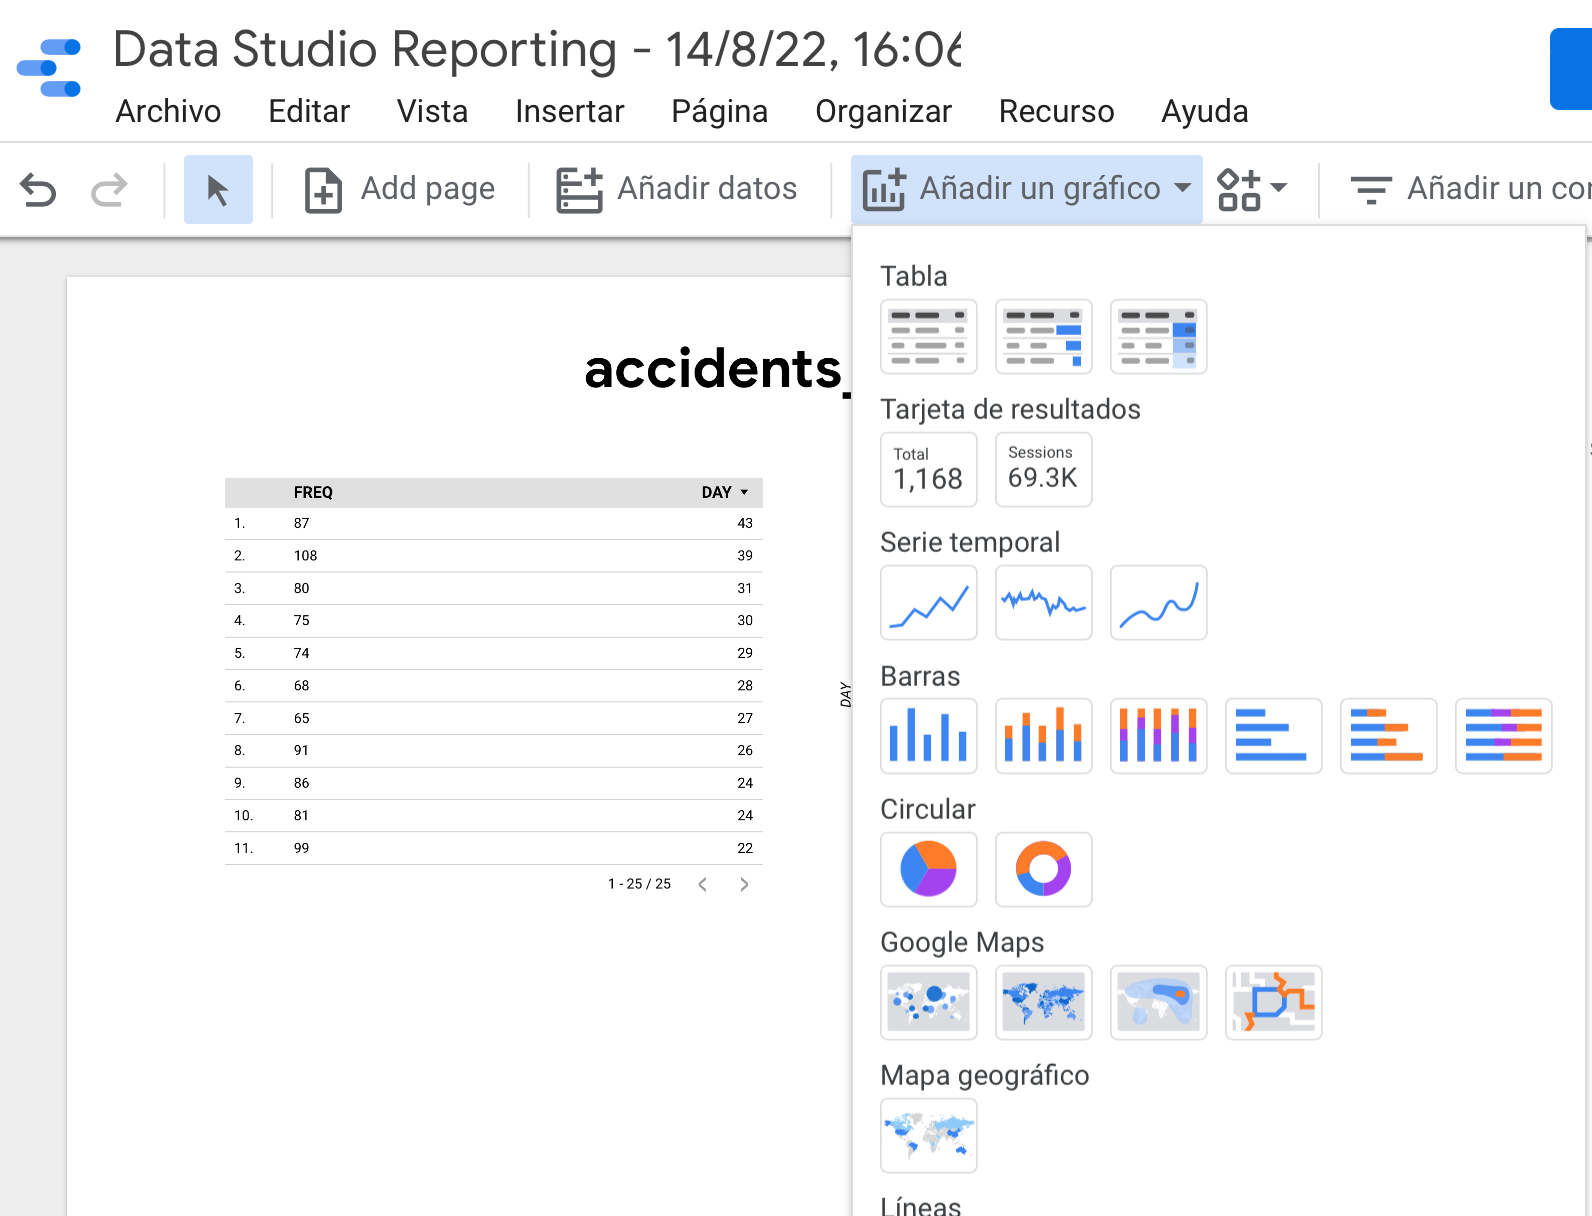
\includegraphics[width=7.25cm]{bq28}}%
\hfill
\raisebox{-.5\height}{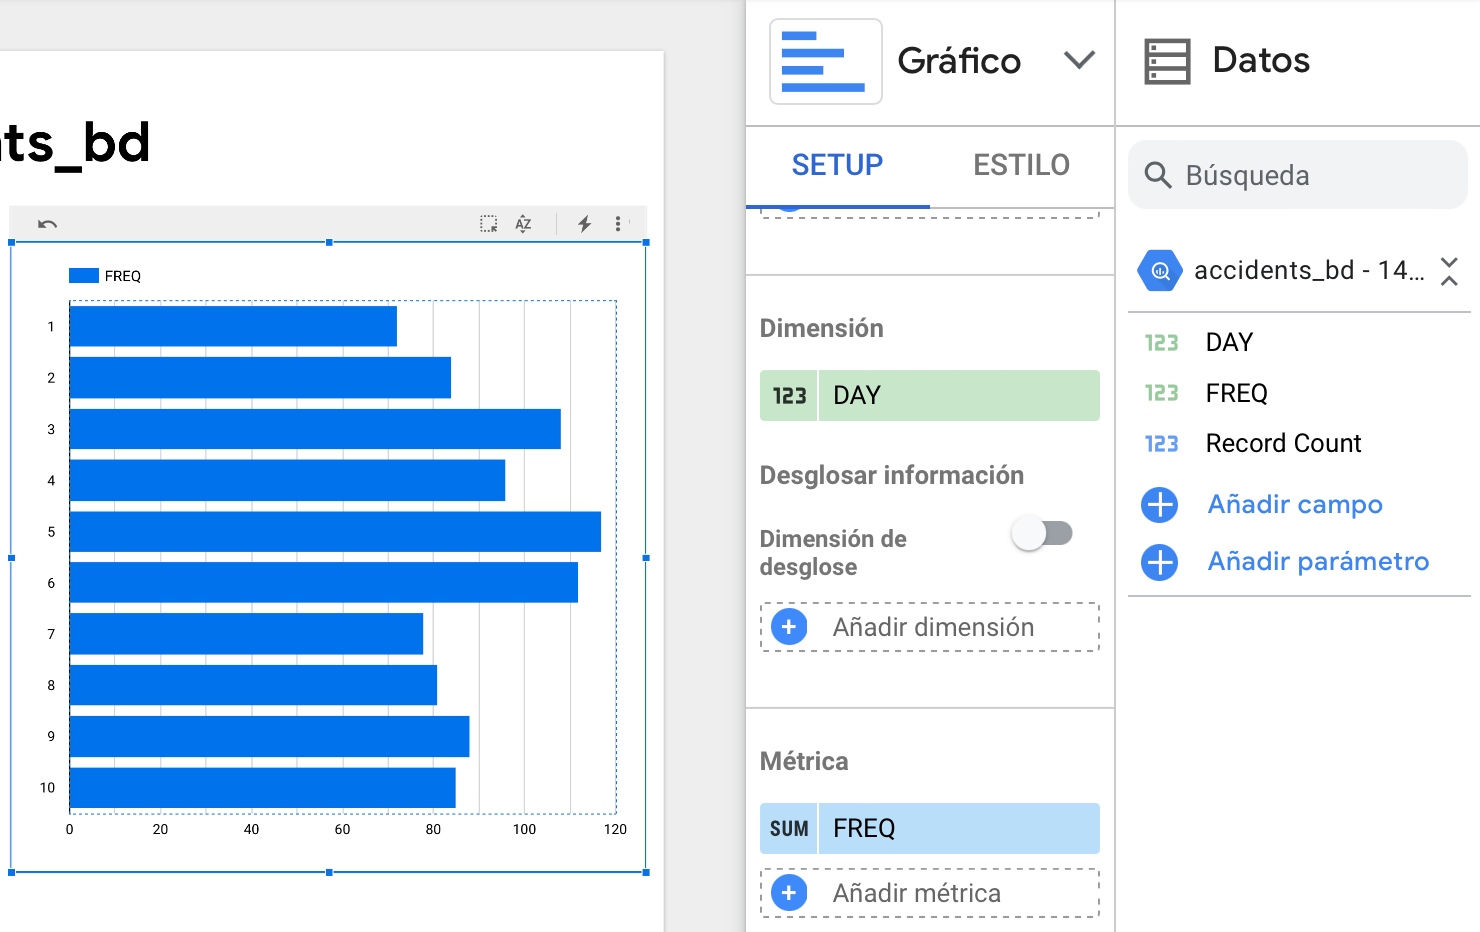
\includegraphics[width=7.25cm]{bq29}}%
\par

\caption{Creació d'un gràfic a partir de Looker Studio}
\label{fig:bq28}
\end{figure}

\subsection{Ús de Looker Studio des de la pròpia plataforma}

Per a utilitzar aquesta eina és necessari disposar d’un compte a Google. Per accedir a la pàgina, naveguem a \href{https://datastudio.google.com}{Looker Studio} i iniciem sessió amb el nostre compte de Google. Un cop dins, es troba una pantalla d’inici amb les característiques següents:

\begin{figure}[h!]
\begin{center}
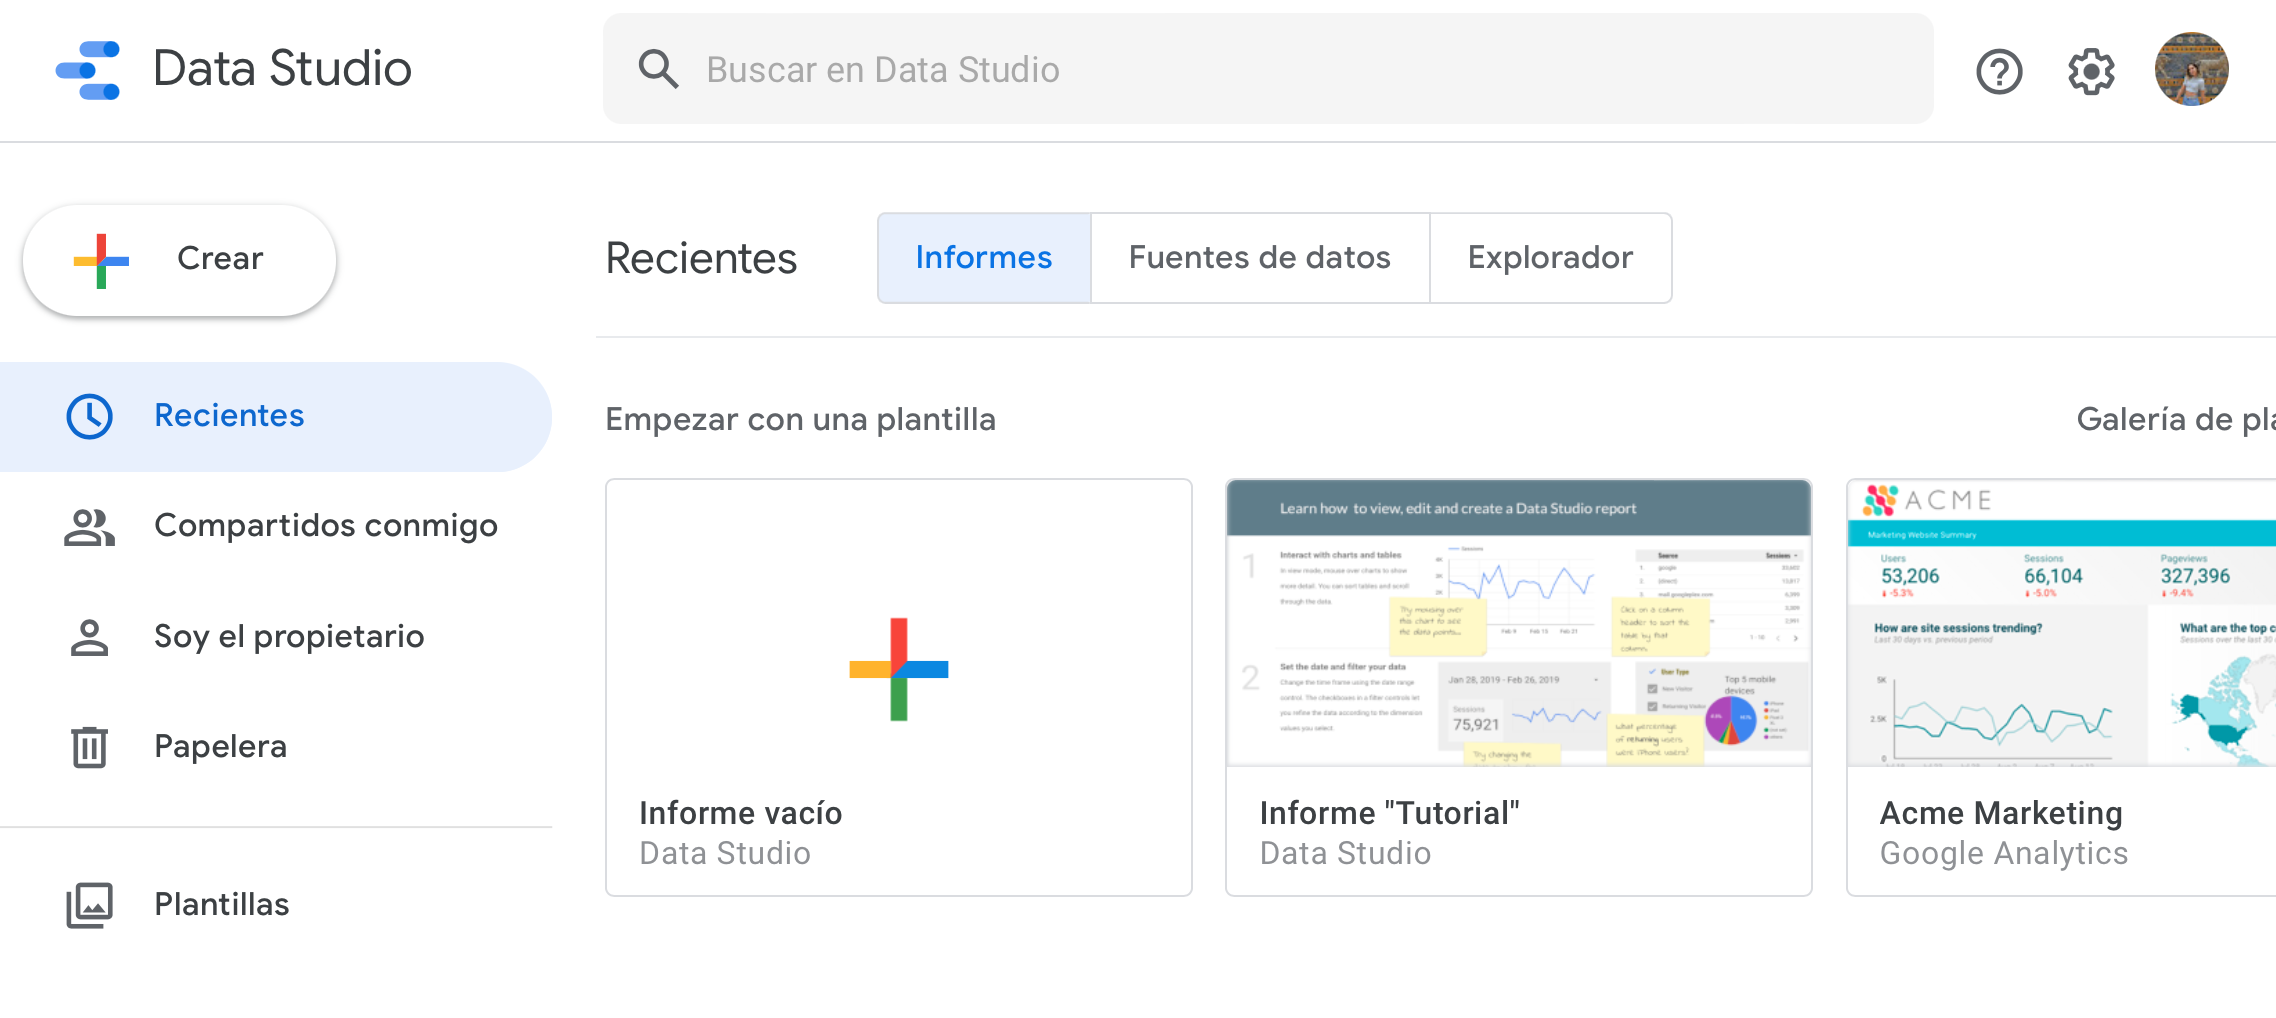
\includegraphics[width=10cm]{ds1}
\end{center}
\caption{Inici de Looker Studio}
\label{fig:ds1}
\end{figure}

A la pàgina d’inici hi ha una sèrie de plantilles, que són una forma entretinguda d’explorar les capacitats de Looker Studio. En el nostre cas, com el que ens interessa és crear un informe des de zero, clicarem a \textit{Informe vacío}. Un cop dins l’informe en blanc, s’hauran d’afegir les dades que volem representar en aquest (Figura ~\ref{fig:ds2}). Tenim moltes opcions a l'hora d'escollir la font de les dades, però per a fer-ho més senzill vincularem l'informe a BigQuery, específicament al nostre conjunt de dades \verb|accidents_bd|.


\begin{figure}[h!]
\par
\raisebox{-.5\height}{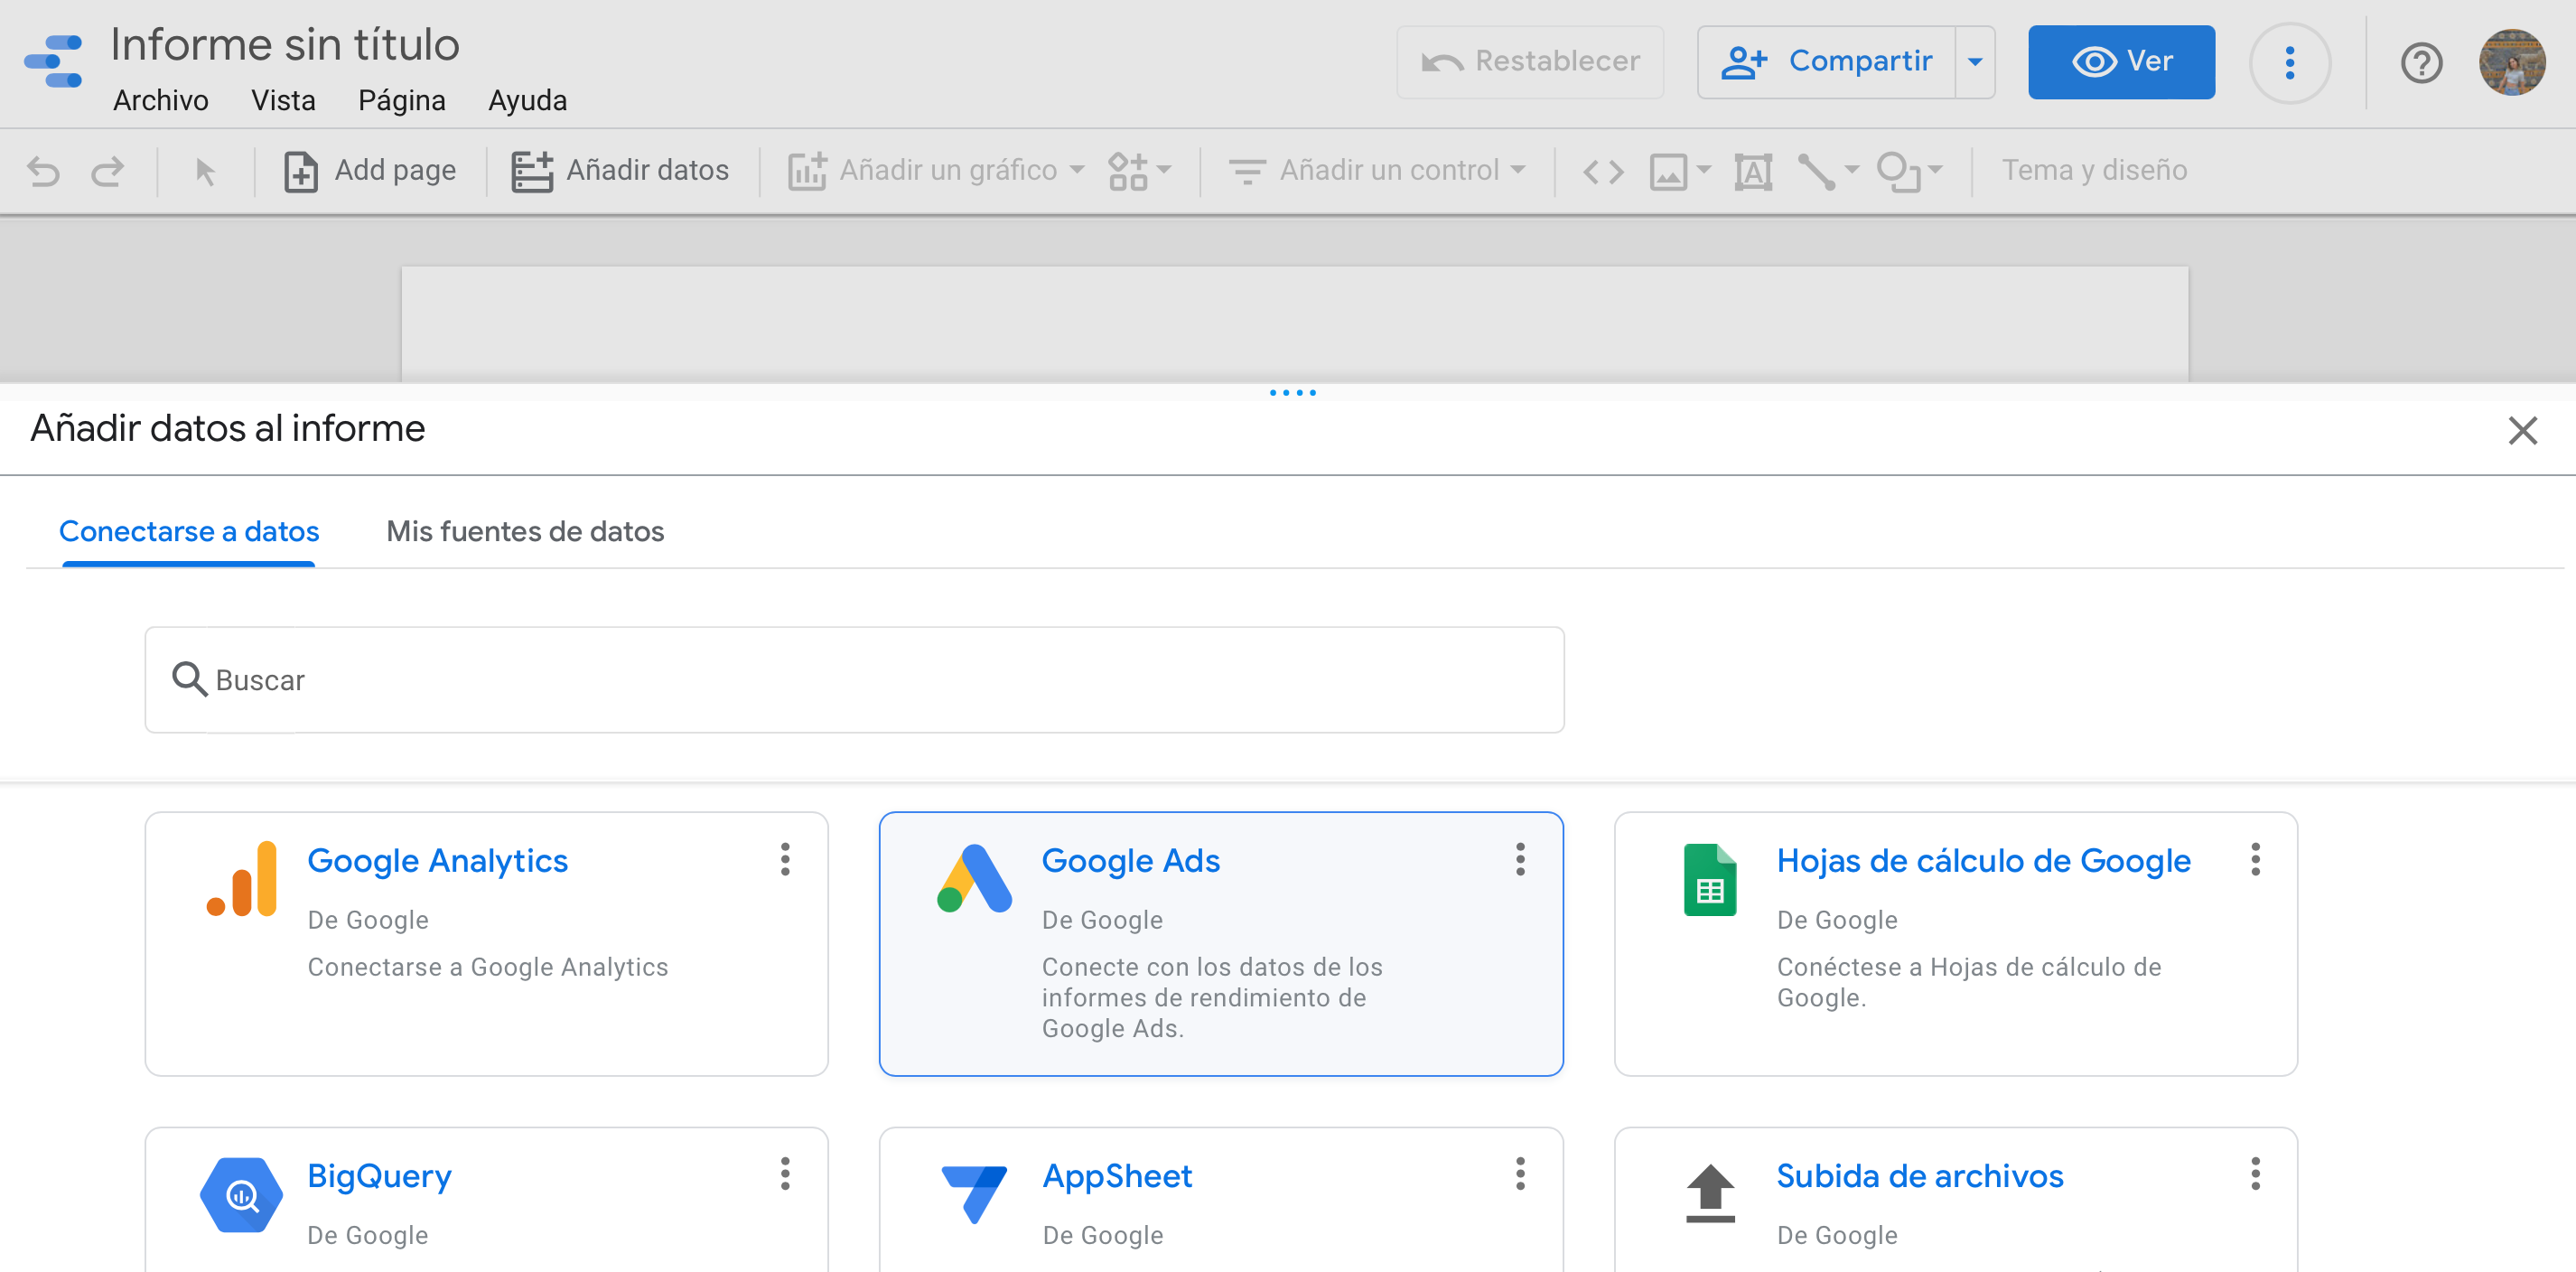
\includegraphics[width=7.25cm]{ds2}}%
\hfill
\raisebox{-.5\height}{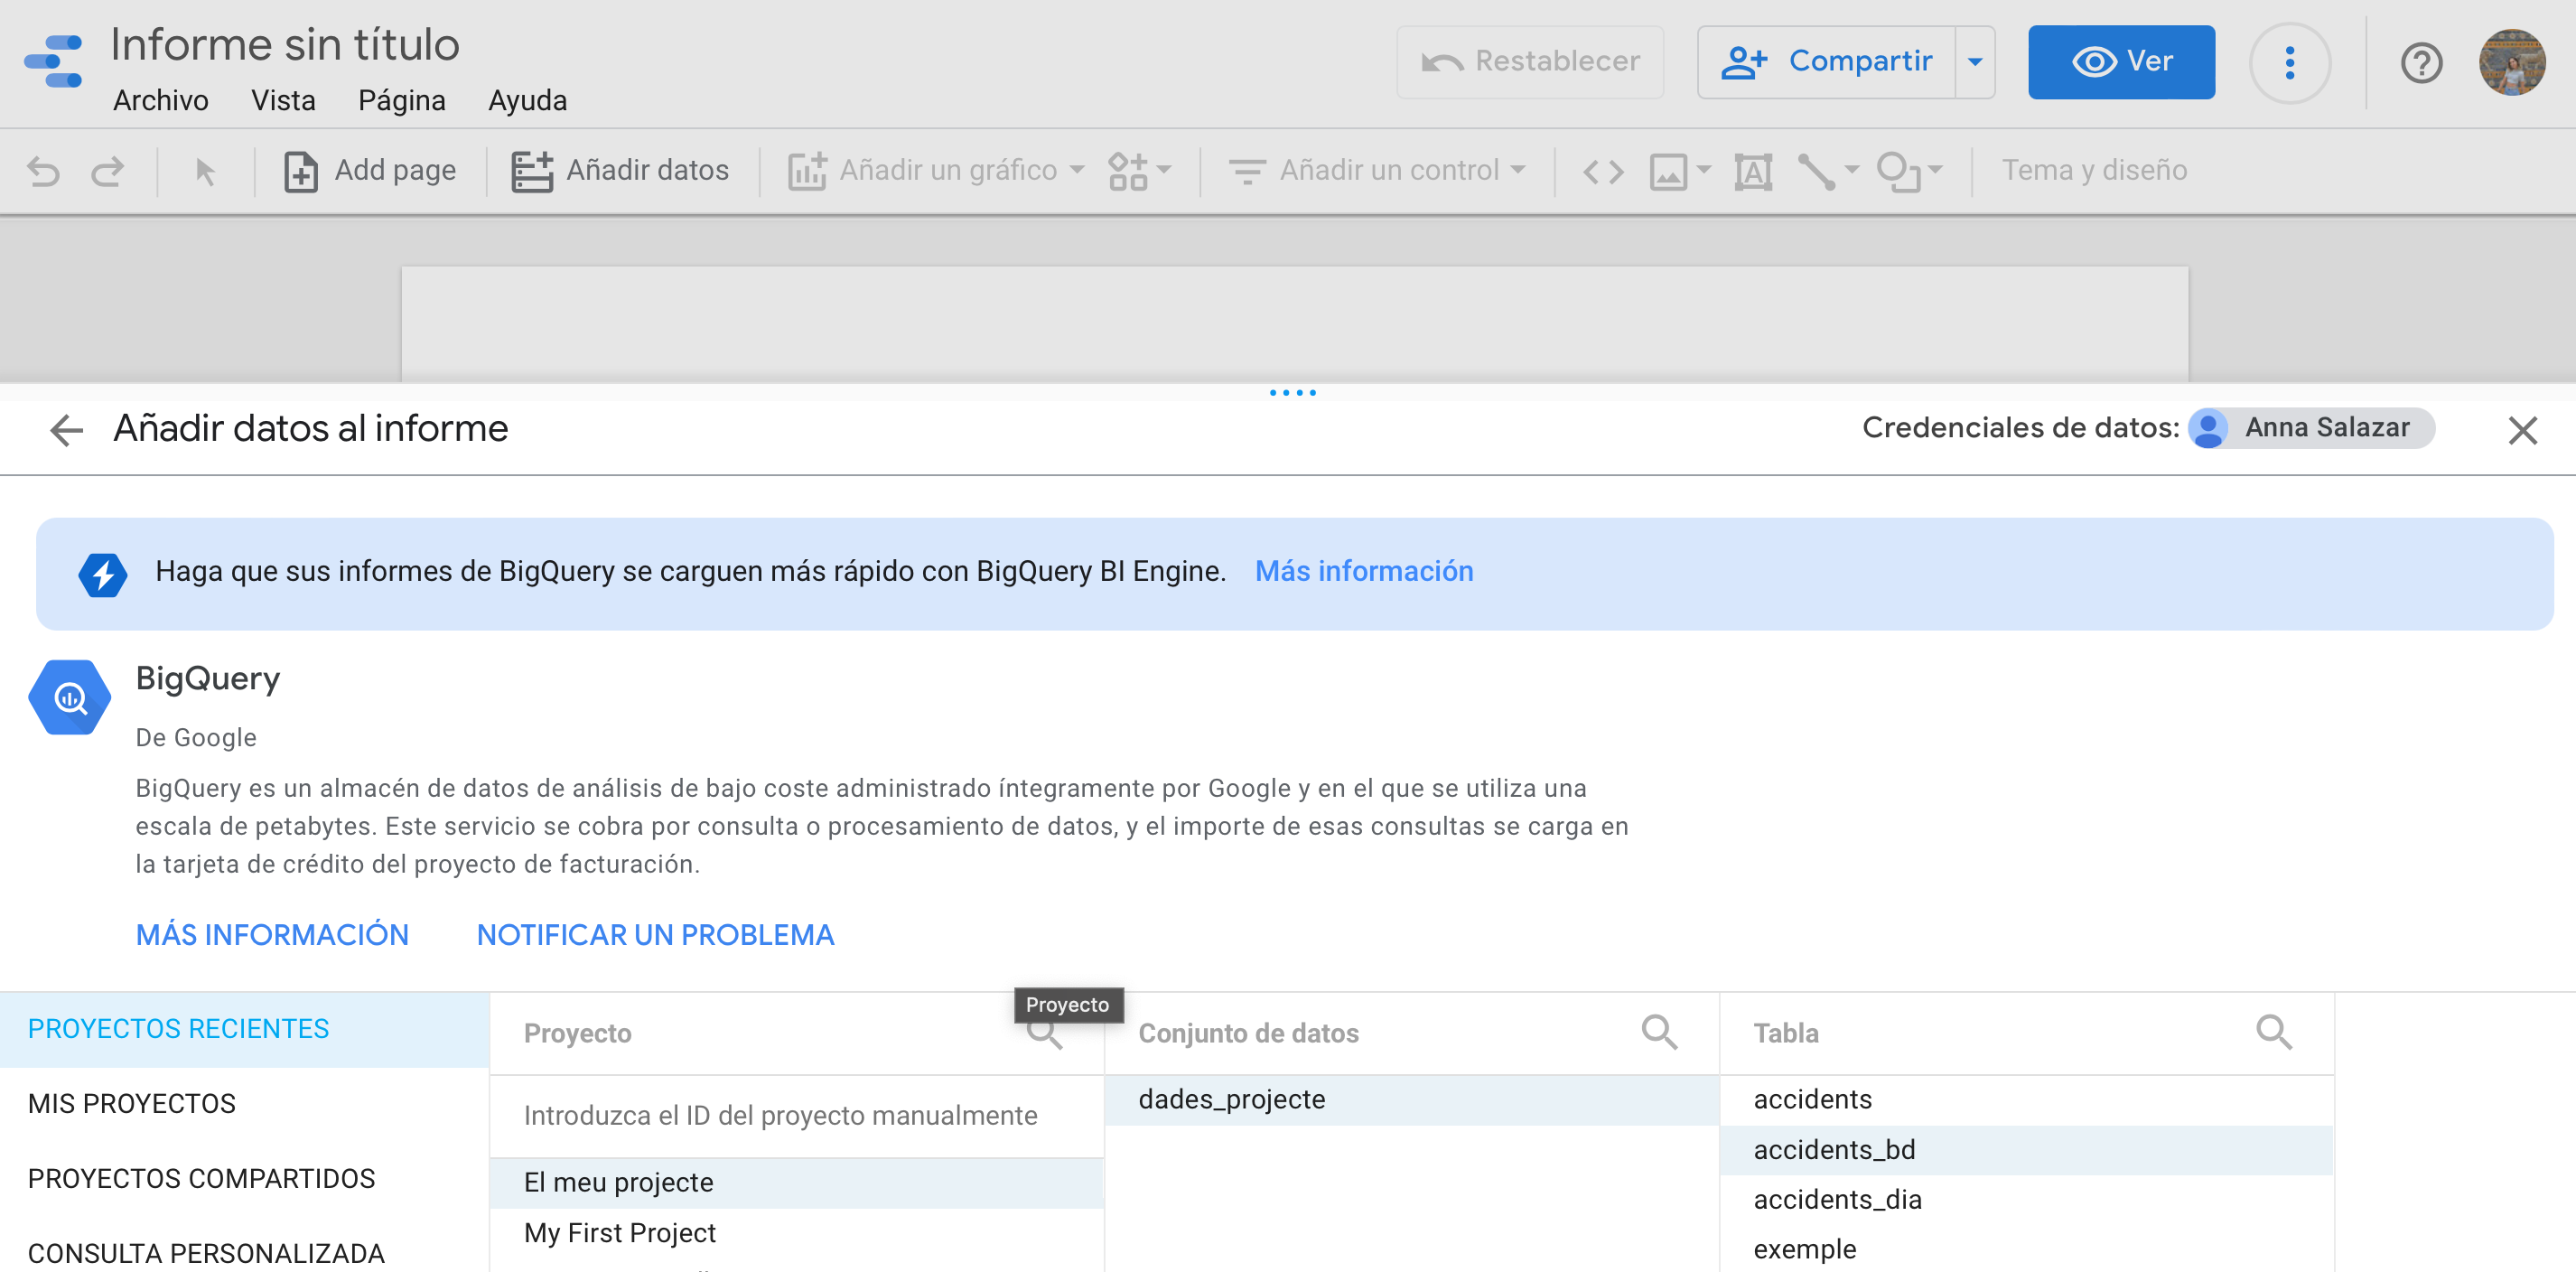
\includegraphics[width=7.25cm]{ds3}}%
\par

\caption{Afegir dades a Looker Studio}
\label{fig:ds2}
\end{figure}

Per a crear un gràfic, podem clicar a \textit{Añadir un gráfico} i, d'aquesta manera, escollir el que ens interessa representar en el panell de la dreta, ajustant la dimensió i la mètrica del nostre interès. Un cop creat el gràfic, es pot editar la seva mida fent-lo més gran o més petit, segons la nostra preferència, i es pot moure de lloc dins la pàgina.

A més de gràfiques, es poden decorar les pàgines per fer-les més boniques, o per afegir informació. També podem afegir un nom a la pàgina, i crear-ne tantes com en necessitem per al nostre informe. Així mateix, podem establir un nom per a tot l'informe, de manera que a l'hora de guardar-lo i compartir-lo sigui més fàcilment interpretable.

Per exemple, un informe de dues pàgines pot tenir un aspecte semblant a la Figura ~\ref{fig:ds4}.

\begin{figure}[h!]
\par
\raisebox{-.5\height}{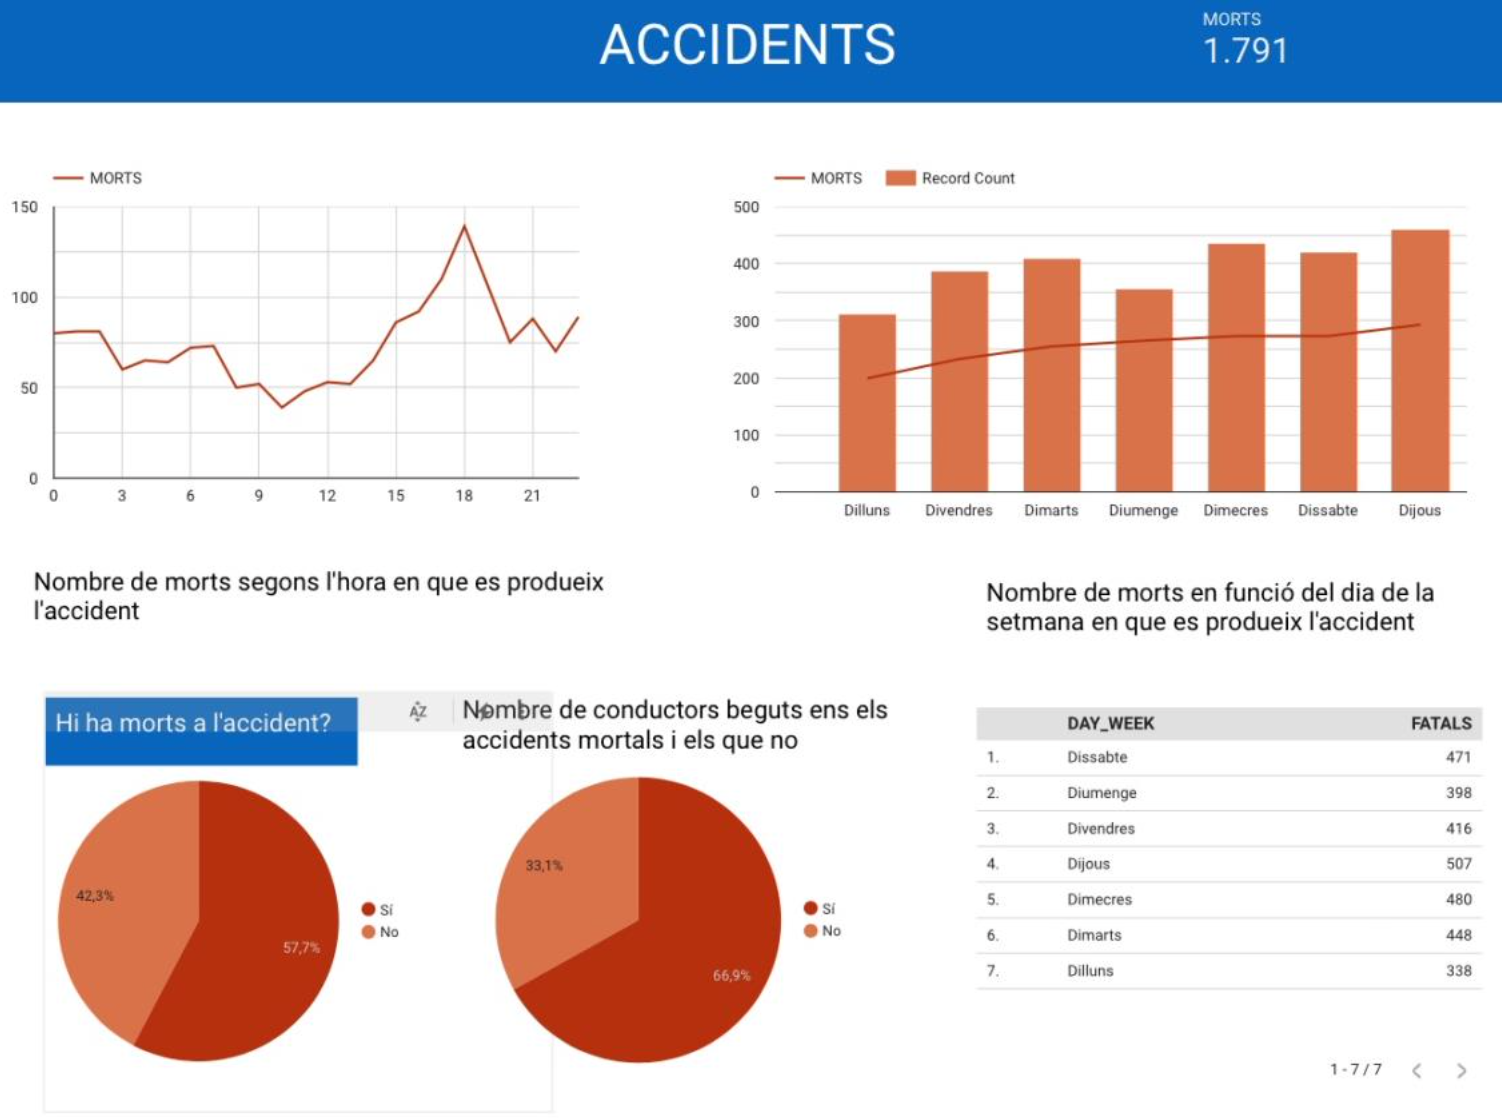
\includegraphics[width=7.25cm]{ds4}}%
\hfill
\raisebox{-.5\height}{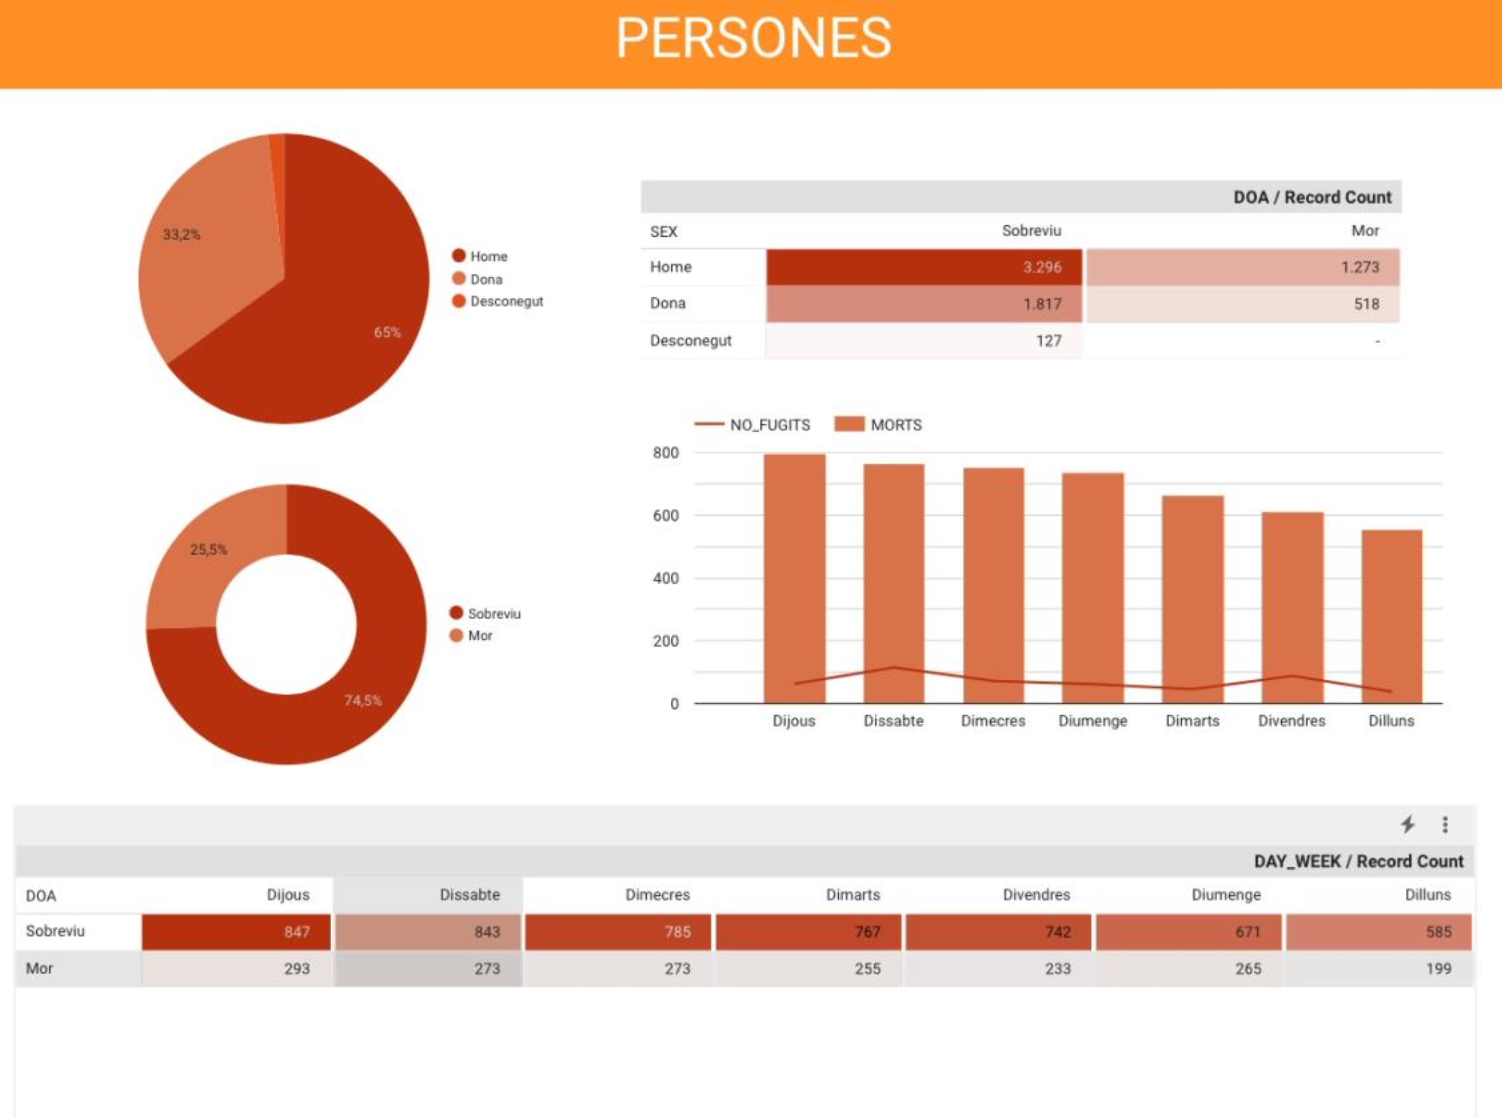
\includegraphics[width=7.25cm]{ds5}}%
\par

\caption{Informe a Looker Studio}
\label{fig:ds4}
\end{figure}


Per acabar, podem compartir el nostre informe perquè altres usuaris puguin tenir accés. Això ho podem fer des de la pantalla d'inici de Data Studio, seleccionant l'opció de compartir l'informe (Figura ~\ref{fig:ds6}) i afegint les adreces de correu dels qui vulguem fer lectors de l'informe (aquells qui poden veure l'informe, però no tenen permisos d'edició) o bé editors (poden veure i editar l'informe). 

\begin{figure}[h!]
\par
\raisebox{-.5\height}{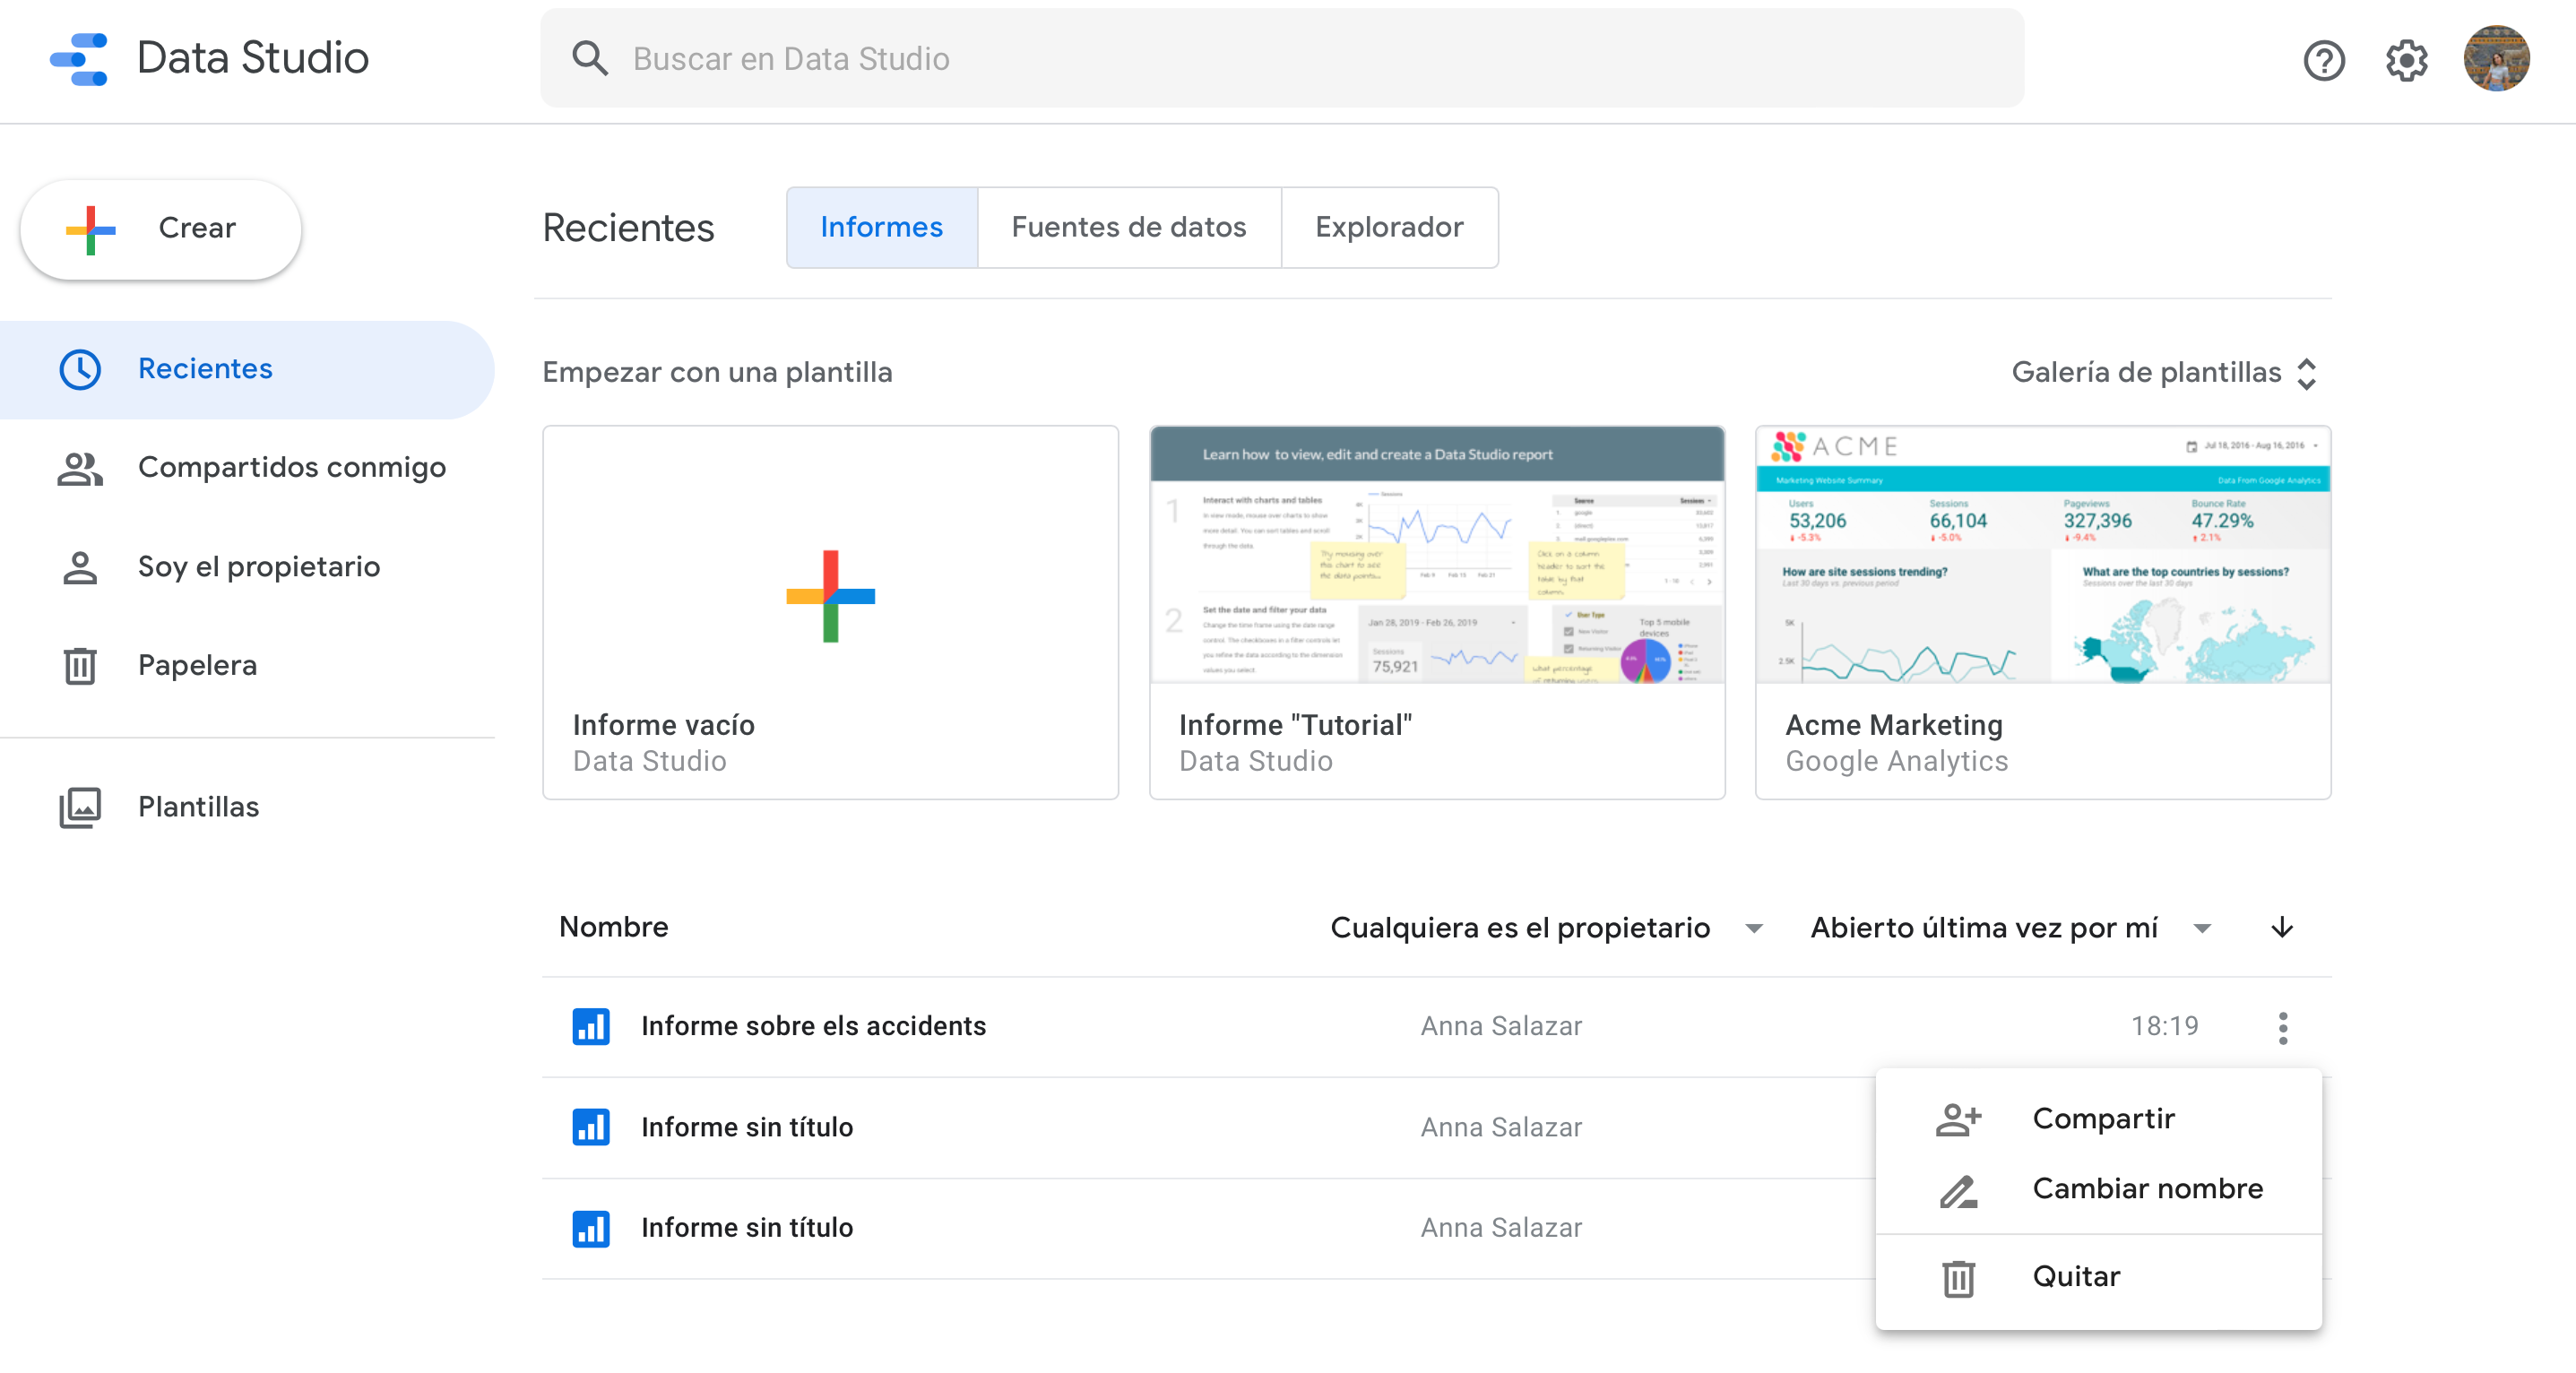
\includegraphics[width=7.25cm]{ds6}}%
\hfill
\raisebox{-.5\height}{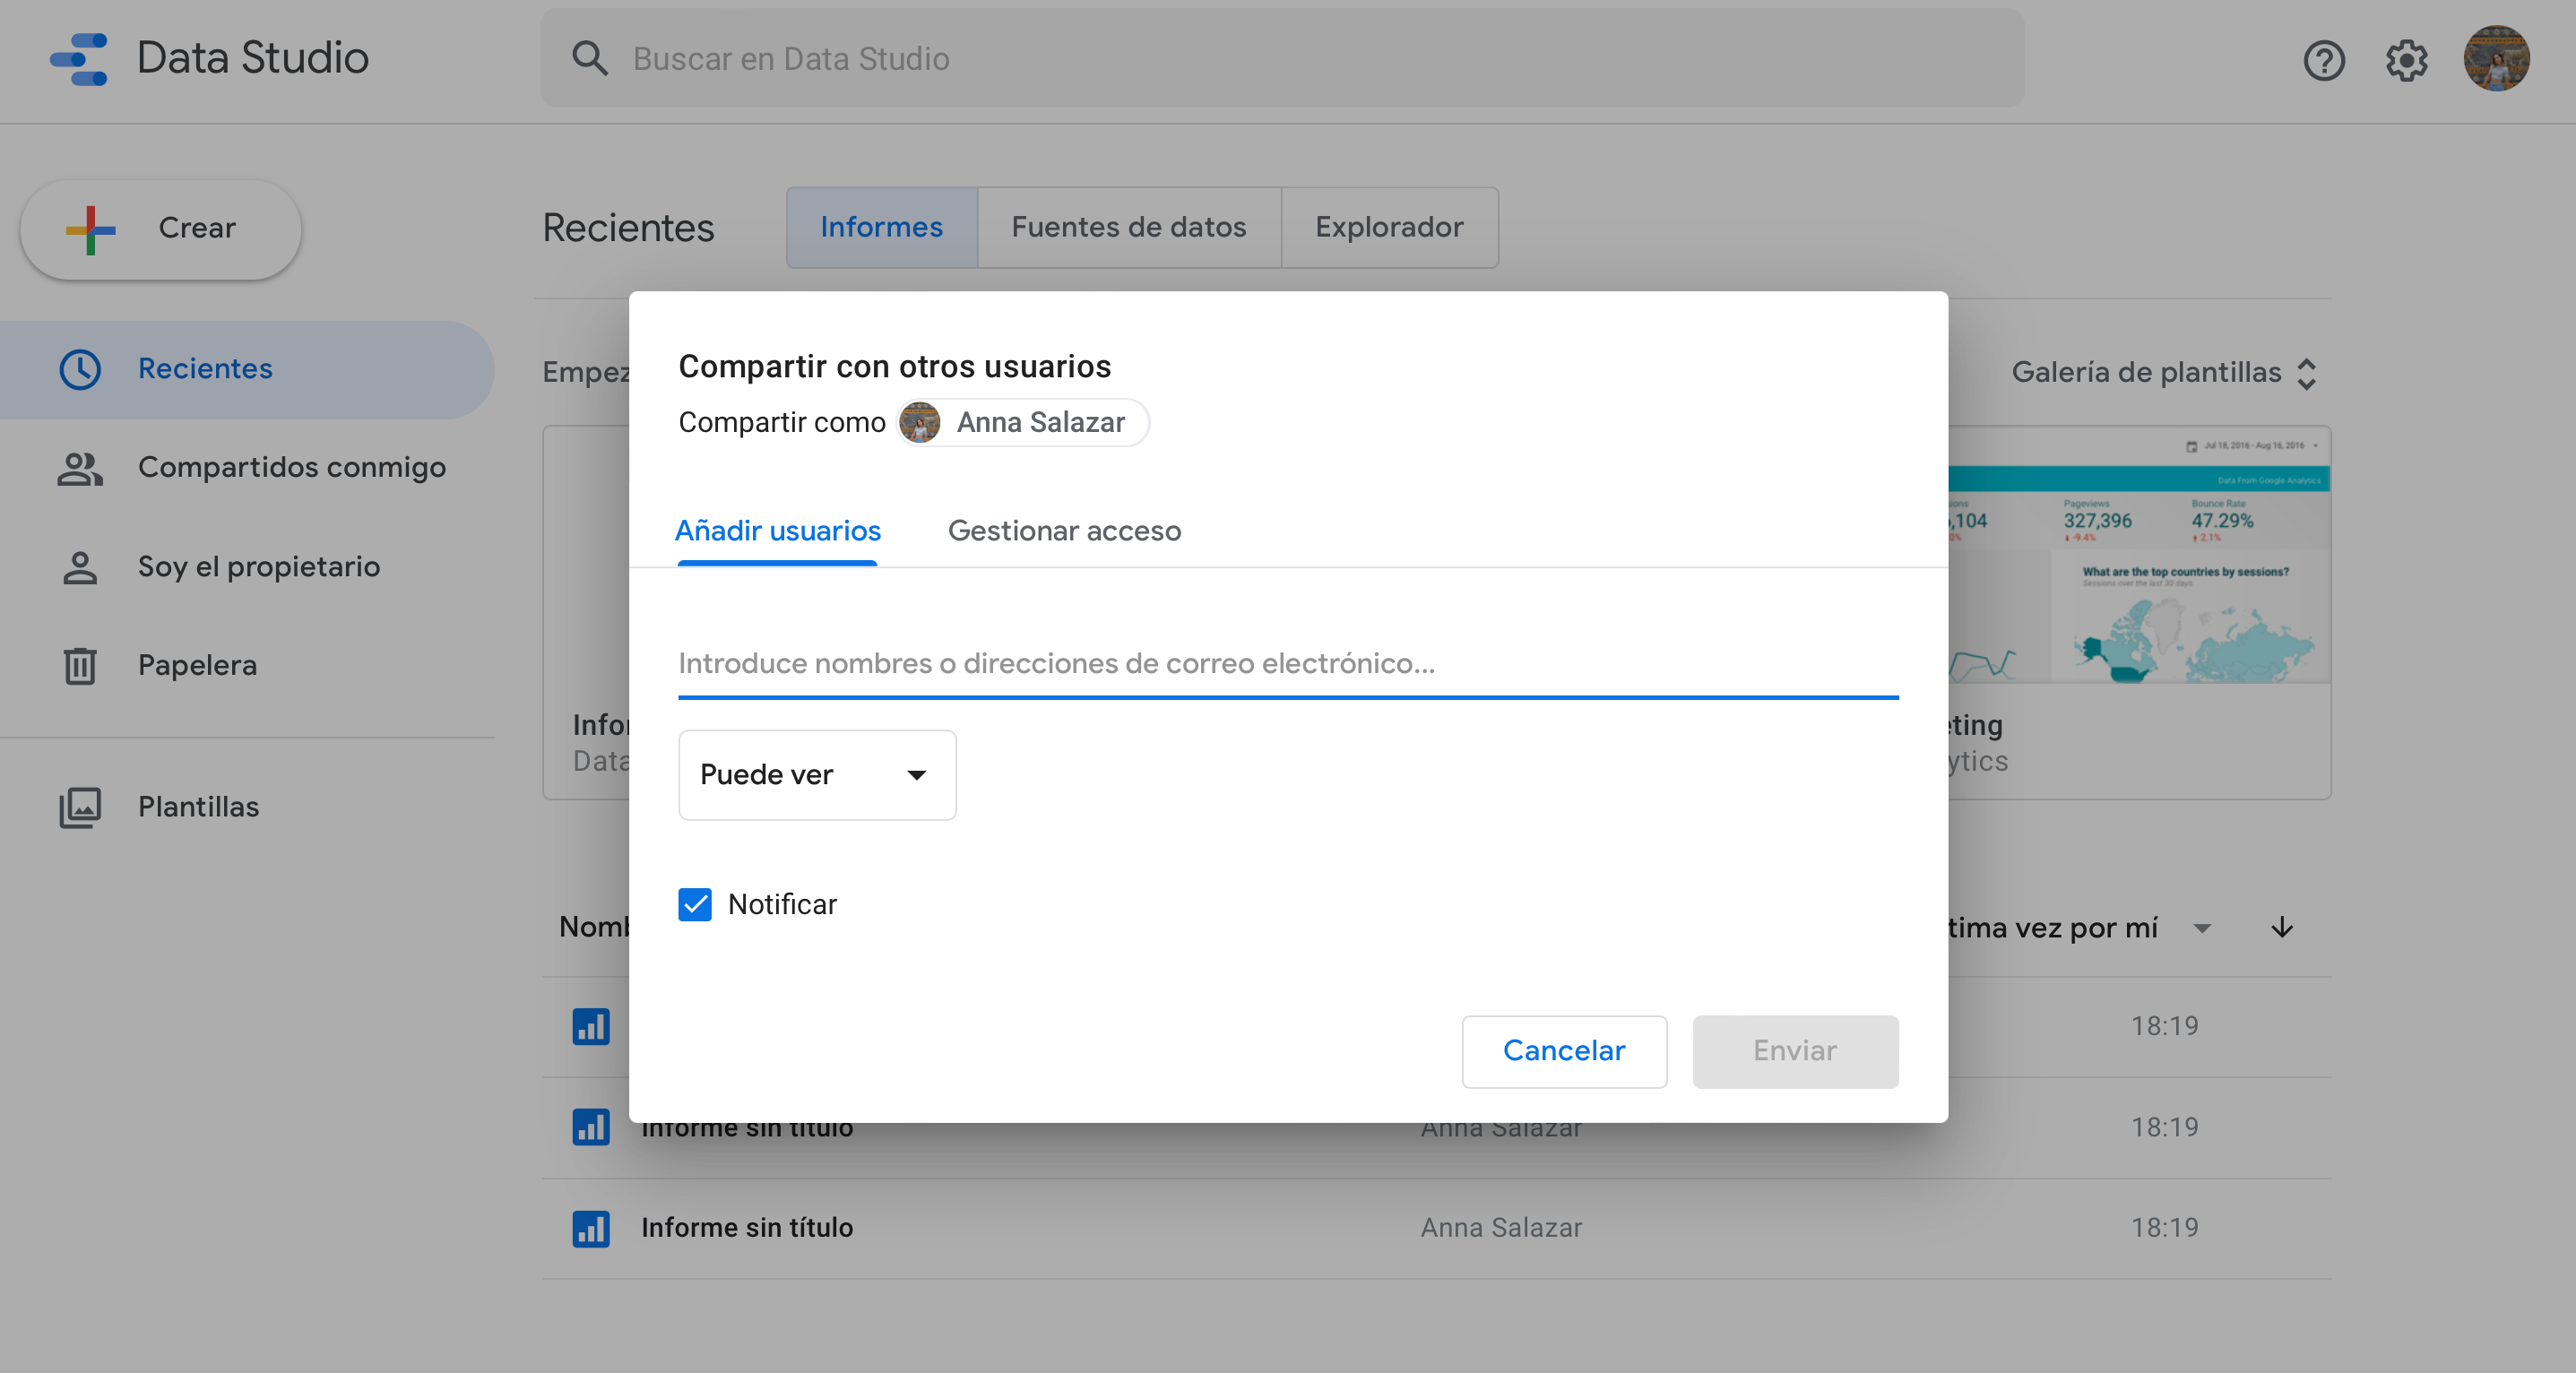
\includegraphics[width=7.25cm]{ds7}}%
\par

\caption{Compartir un informe}
\label{fig:ds6}
\end{figure}

\newpage

\section{Connexió d'R a BigQuery}

\subsection{Connectem R a BigQuery}

Per a entendre com funciona la connexió entre BigQuery i R, primer s'ha de definir el concepte de \emph{API} o interfície de programació d'aplicacions.


Una API és un conjunt de processos, funcions i mètodes que ofereix una determinada biblioteca de programació que serveix com a capa d'abstracció perquè sigui emprada per un altre programa informàtic. Dit d'una altra manera, podem entendre les APIs com un codi que indica a les aplicacions com comunicar-se entre elles, de manera que puguin interactuar.


En el nostre cas, volem que R sigui capaç d'interactuar amb BigQuery, perquè així ens permeti realitzar les nostres consultes a la base de dades sense haver d'importar les dades a R. Haurem d'utilitzar les llibreries \texttt{bigrquery}\footnote{Una interfície per a la API de 'BigQuery' de Google} i \texttt{DBI}\footnote{Una definició d'interfície de base de dades per a la comunicació entre R i els sistemes de gestió de bases de dades relacionals (SGBD). Totes les classes d'aquest paquet són virtuals i han de ser esteses per les diferents implementacions de R/SGBD.} per aconseguir-ho. 

\begin{verbatim}
install.packages("bigrquery")
install.packages("DBI")
library(bigrquery)
library(DBI)
\end{verbatim}

Asignem a l'objecte \texttt{projecte} el nom del nostre projecte, que a l'exemple correspon a \emph{el-meu-} \emph{projecte-358912}.

\begin{verbatim}
projecte <- "el-meu-projecte-358912"
\end{verbatim}

I per últim, mitjançant la funció \texttt{dbConnect()} obrirem la connexió amb Bigquery indicant el nom del nostre projecte i la base de dades a la que volem accedir dins d'aquest, \texttt{dades\_projecte}. A l'apartat \emph{billing} s'haurà d'introduir l'identificador del projecte amb la font de facturació. Nosaltres indiquem el nom del nostre projecte, que està sotmès a les limitacions de la \emph{Sandbox} o zona de proves gratuïta.

\begin{verbatim}
dades <- dbConnect(
  bigrquery::bigquery(),
  project = projecte,
  dataset = "dades_projecte",
  billing = projecte
)
\end{verbatim}

Executant aquest codi no es produeix gran cosa, tret que es crea una variable de connexió. Però la primera vegada que intentem fer ús d'aquesta connexió (per exemple, fent una consulta a una de les taules de la base de dades), se'ns demana que ens autentifiquem a través del nostre compte de Google en una finestra del navegador. Un cop fet això, ja podrem començar a consultar les nostres dades de BigQuery, així com els conjunts de dades públics. 


\subsection{Consultes amb `bigrquery`}

Per a mostrar com seria una cosulta a la nostra taula des de R buscarem el llistat d'accidents que van ocórrer un cap de setmana a les 21:00.

\begin{verbatim}
query1 <- "SELECT ST_CASE 
           FROM `el-meu-projecte-358912.dades_projecte.accidents_bd`
           WHERE (DAY = 1 or DAY = 7) and HOUR = 21 and MINUTE = 0"
\end{verbatim}

Un cop hem formulat la nostra \emph{query}, a través de la funció \texttt{dbGetQuery()}, ens comunicarem amb la API de Google. 

\begin{multicols}{2}

\begin{verbatim}
dbGetQuery(connexió, consulta, n)
\end{verbatim}

\columnbreak

\begin{verbatim}
dbGetQuery(dades, query1, n = 10)
\end{verbatim}

\end{multicols}

Essent \emph{n} el nombre de casos a mostrar (si calen restriccions).


En executar aquesta consulta, R retorna la següent taula:

\begin{table}[h]
\centering
\begin{tabular}{|c|}
\hline
\textbf{ST\_CASE} \\ \hline
62353             \\ \hline
\end{tabular}
\end{table}

Aquesta correspon a que únicament va ocórrer un accident un cap de setmana a les 21:00, i aquest té l'identificador \texttt{62353}.

\newpage



\section{Implementació de BigQuery a l'aula}

BigQuery és una eina d'anàlisi de dades d'alt rendiment, capaç de processar un volum molt gran d'informació en segons, és senzill d'utilitzar i ofereix la zona de proves des de la que es pot treballar de forma gratuïta. És per aquest motiu que s'ha presentat aquest programa als estudiants del grau d'estadística a l'assignatura de Fitxers i Bases de Dades, perquè ells mateixos puguin avaluar la seva experiència amb la plataforma de Google Cloud, així com el grau de dificultat que troben en el seu ús.

Per portar a terme aquesta dinàmica es van necessitar dues sessions de dues hores cadascuna. A la primera, es va presentar tota la informació teòrica sobre la plataforma. S'explicava les propietats de BigQuery, així com les limitacions que presenta la seva zona de proves. La professora Montserrat Guillén va fer unes diapositives per presentar-les a l'aula on s'incorporava tota la informació necessària per crear-se un compte a BigQuery i poder dur a terme l'activitat proposta. Aquestes diapositives van ser creades a partir de la recerca contemplada en aquest treball, i en elles es van fer algunes modificacions a l'hora de penjar-les al campus virtual, per evitar publicar un material que encara no s'havia presentat.


\subsection{Consultes amb `bigrquery`}


Per portar a terme la sessió pràctica es va fer ús del conjunt de dades públic prèviament esmentat: \emph{Catalonia Cell Coverage}, que contenen informació sobré l'estat de cobertura de la telefonia mòvil que es va recollir en el periode dels anys des del 2015 fins al 2017.


En primer lloc es presetava la taula de dades amb la qual s'havia de treballar, que conté les variables següents:


\begin{longtable}[H]{p{.20\textwidth} | p{.80\textwidth} } 
\textbf{Variable} & \textbf{Descripció}                              \\ 
date              & Data de telemetria en format AAAA-MM-DD          \\
hour              & Hora de telemetria en format HH24:MM:SS          \\
lat               & Latitud                                          \\
long              & Longitud                                         \\
signal            & Senyal mitjana                                   \\
network           & Nom de la xarxa                                  \\
operator          & Nom de l'operador                                \\
status            & Codi de l'estat = \{0, 1, 2, 3\}                 \\
description       & Descripció de l'estat                            \\
                  & - En servei (0)                                  \\
                  & - Fora de servei (1)                             \\
                  & - Estat d'emergència (2)                         \\
                  & - Apagat                                         \\
net               & Tipus de xarxa = 2G, 3G, 4G                      \\
speed             & Velocitat estimada de la font                    \\
satellites        & Nombre de satèl·lits GPS                         \\
precission        & Constant que decriu la precisió del proveïdor    \\
provider          & Nom del proveïdor de la posició                  \\
activity          & Activitat de l'usuari:                           \\
                  & - En un vehicle                                  \\
                  & - Parat                                          \\
                  & - A peu                                          \\
                  & - Inclinat                                       \\
                  & - Amb bicicleta                                  \\
                  & - Desconegut                                     \\
downloadSpeed     & Velocitat de descàrrega actual                   \\
uploadSpeed       & Velocitat de càrrega actual                      \\
postal\_code      & Codi postal                                      \\
town\_name        & Nom de la ciutat on es va adquirir la telemetria \\
position\_geom    & Representació gràfica de la posició         \\
\caption{Variables de les dades Catalonia Cell Coverage}
\label{tab:CCC}
\end{longtable}

Un cop els estudiants es trobaven a l'entorn BigQuery, les consultes a crear havien de resoldre les demandes següents:

\begin{enumerate}

\item Feu una taula de freqüències de l'activitat que fa cada usuari segons les dades recollides.

\begin{Verbatim}[frame=single]

SELECT activity, count(date) AS Freq
FROM `bigquery-public-data.catalonian_mobile_coverage_eu.
      mobile_data_2015_2017`
GROUP BY activity

\end{Verbatim}

\item Retorneu un llistat de les 5 ciutats amb millor connexió mitjana de Catalunya.

\begin{Verbatim}[frame=single]

SELECT AVG(SIGNAL) AS AVG_SIGNAL, TOWN_NAME
FROM `bigquery-public-data.catalonian_mobile_coverage_eu.
      mobile_data_2015_2017`
GROUP BY TOWN_NAME
ORDER BY AVG_SIGNAL DESC
LIMIT 5

\end{Verbatim}

\item Feu un resum numèric (mínim, mitjana, desviació típica i màxim) de la precisió de la xarxa per aquelles 10 que tenen la mitjana més elevada.

\begin{Verbatim}[frame=single]

SELECT network, min(precission) AS Minim, avg(precission) AS 
Mitjana, stddev(precission) AS Desv_Tipica, max(precission) AS 
Maxim
FROM `bigquery-public-data.catalonian_mobile_coverage_eu.
      mobile_data_2015_2017`
GROUP BY network
ORDER BY Mitjana DESC
LIMIT 10

\end{Verbatim}

\item Creeu una taula que reculli les ciutats i la xarxa dels 10 primers usuaris que es van quedar sense servei mòvil, obviant els casos en què el nom de la ciutat o de la xarxa sigui \textit{NULL}.

\begin{Verbatim}[frame=single]

SELECT town_name, network
FROM `bigquery-public-data.catalonian_mobile_coverage_eu.
      mobile_data_2015_2017`
WHERE description="STATE_OUT_OF_SERVICE" AND 
      town_name IS NOT NULL AND network IS NOT NULL
ORDER BY date ASC
LIMIT 10

\end{Verbatim}

\item Construiu una taula que reculli la xarxa, el seu tipus i la precisió mitjana. Llisteu els 10 primers casos, en ordre descendent, segons la precisió mitjana.

\begin{Verbatim}[frame=single]

SELECT network, net, avg(precission) AS Precisio_mitj
FROM `bigquery-public-data.catalonian_mobile_coverage_eu.
      mobile_data_2015_2017`
WHERE precission IS NOT NULL AND 
      net IS NOT NULL AND network IS NOT NULL
GROUP BY network, net
ORDER BY Precisio_mitj DESC
LIMIT 10

\end{Verbatim}

\item Feu un gràfic de sectors sobre l'aparició dels diferents tipus de xarxa, excloent els casos en què aquesta variable pren el valor \textit{NULL}.

\vspace{2mm}
\begin{figure}[H]
\begin{center}
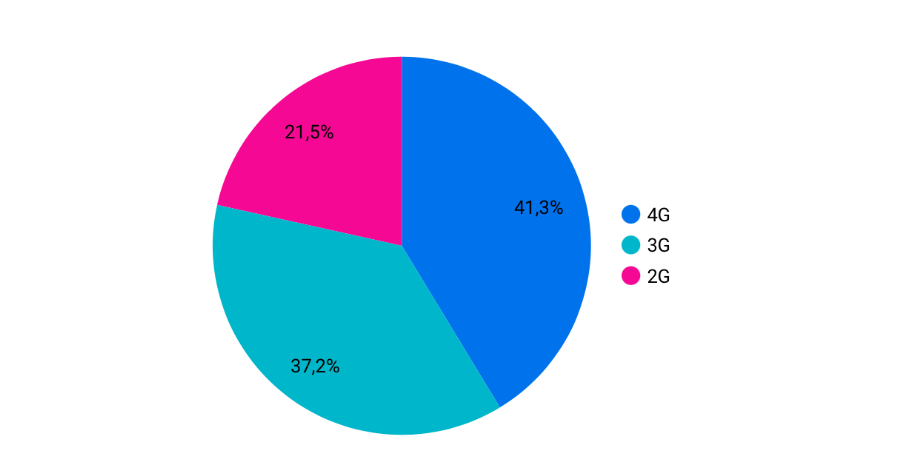
\includegraphics[width=12.5cm]{pbq1}
\end{center}
\label{fig:pbq1}
\end{figure}

\item Creeu un histograma que mostri la freqüència en què apareix cada operador a la base de dades. Utilitzeu Looker Studio per a fer-ho.

\vspace{2mm}
\begin{figure}[H]
\begin{center}
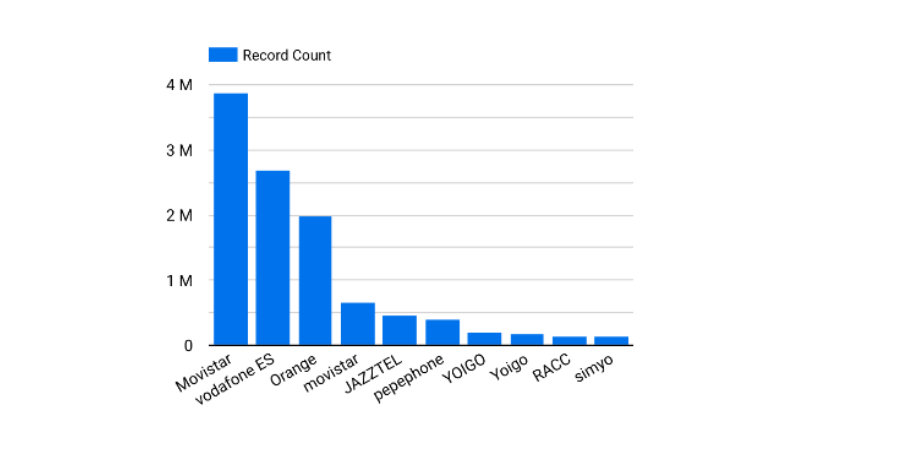
\includegraphics[width=12.5cm]{pbq2}
\end{center}
\label{fig:pbq2}
\end{figure}

\end{enumerate}

\subsection{Comentaris del estudiants sobre la pràctica}

D'entre els estudiants matriculats a l'assignatura de Fitxers i Bases de Dades, van ser vint-i-un els qui van realitzar la pràctica i van valorar la seva interacció amb BigQuery. Les preguntes que van respondre aquests estudiants eren:


Responeu a les següents preguntes sobre l'ús de BigQuery. Valoreu (0: molt fàcil - 10: molt difícil)


\begin{enumerate}

\item Entorn BigQuery (connexió)

\item Entorn BigQuery (consultes SQL)

\item Connexió amb R

\item Valoració global

\end{enumerate}

\begin{itemize}

\item Suggeriu alguna milora en la introducció a BigQuery?

\end{itemize}

A continuació es farà una recopilació dels resultats obtinguts, d'on es pot veure un resum numèric a la figura \ref{ig:val}.

\begin{figure}[h!]
\begin{center}
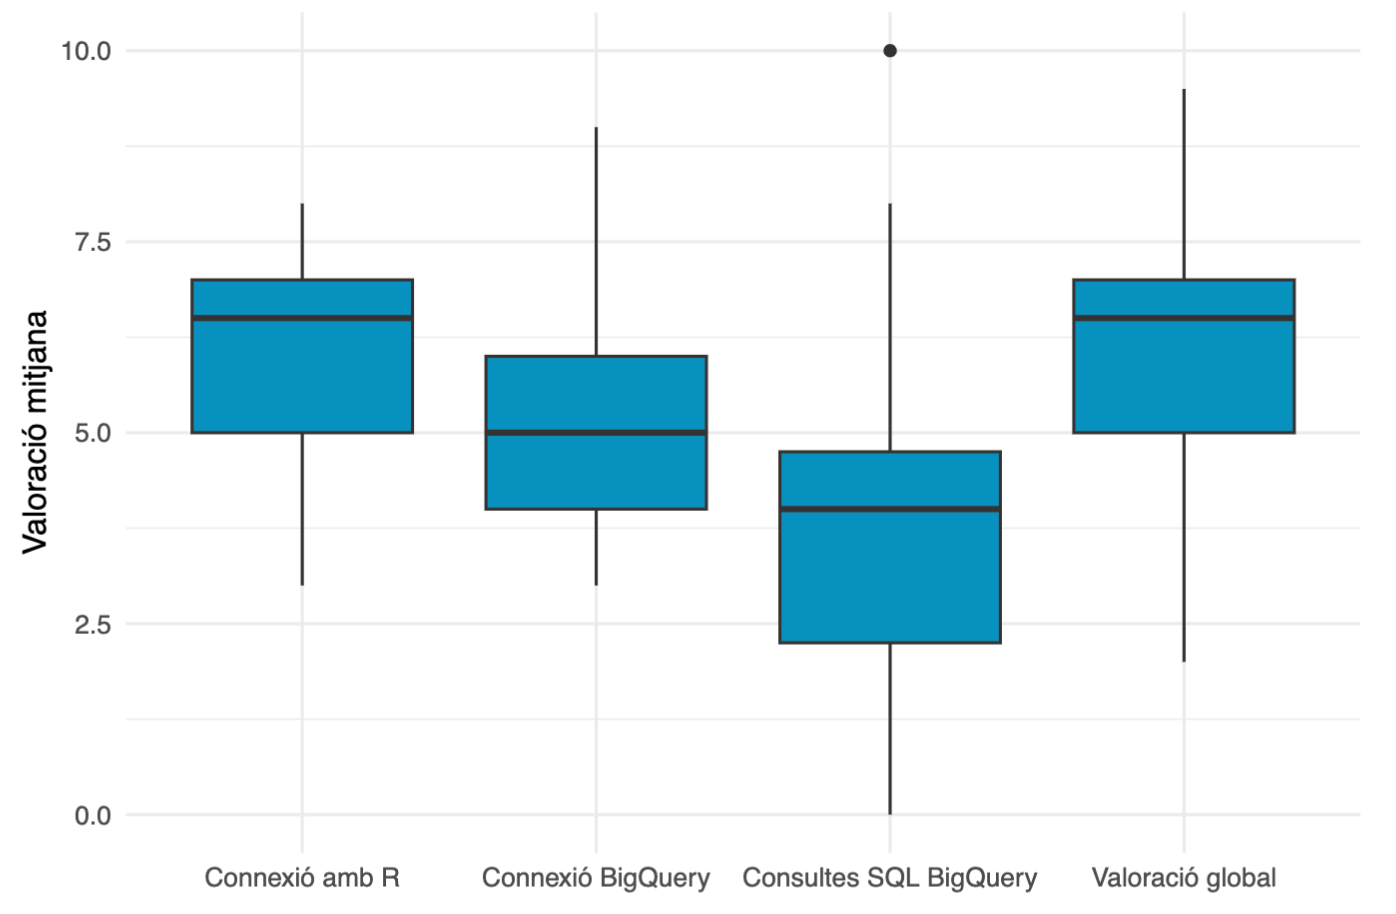
\includegraphics[width=13.5cm]{val}
\end{center}
\caption{Valoració mitjana dels estudiants}
\label{fig:val}
\end{figure}



Pel que fa a la connexió a BigQuery, la puntuació mitjana va ser de 5,44. Els estudiants no ho consideren fàcil, però tampoc li troben un grau de dificultat molt elevat a connectar-se a la plataforma per primera vegada. Alguns comenten que, en ser un entorn nou, els hi costa perquè no hi estan familiaritzats i els fa sortir de la seva zona de comfort.


En relació a les consultes SQL (\textit{Structured Query Language}) a l'entorn BigQuery, la puntuació mitjana baixa a 4,06. És a dir, als estudiants, en general, els sembla més senzill l'ús de BigQuery que l'entrada a la plataforma. El llenguatge que s'utilitza a BigQuery és molt similar a d'altres vistos a ACCES, R o SAS, i així ho fan saber els estudiants.


En quant a la connexió amb R, la puntuació mitjana ha sigut de 6, una mica més elevada que les anteriors. S'ha trobat una mica més de complicació en aquest punt, ja que el funcionament de les APIs no s'havia tractat prèviament i era un concepte nou.


Per últim, la valoració global ha estat de 6,09 en quant a la dificultat del programa.


També s'ha preguntat si els estudiants volien deixar suggerències per la millora en la introducció a BigQuery, aquelles coses que canviarien i/o els hi facilitaria la introducció a aquesta eina. Molts dels comentaris que s'han repetit en les valoracions és que els hi hagués ajudat el fet de dedicar-hi més pràctiques, perquè suposava un volum de informació molt gran que se'ls hi ha explicat en poc temps. A més, demanden que l'explicació de la teoria vingui acompanyada d'un suport pràctic des de la primera sessió, per entendre millor des del principi el funcionament de BigQuery.


Tot i que aquesta mostra d'estudiants difícilment és representativa, perquè només han participat vint-i-un estudiants a les sessions pràctiques, els resultats han sigut força positius i els estudiants han mostrat a les valoracions el seu interès en seguir coneixent aquest tipus d'eines, perquè els hi semblen interessants de cara al futur.


\newpage


\section{Anàlisi de dades mitjançant la connexió d'R i BigQuery}

\subsection{Descripció de la base de dades}

La base de dades que serà utilitzada al llarg de l'estudi provené de l'agència estatal de trànsit dels Estats Units i contené tres taules, entre les quals es troba un llistat d’accidents de trànsit ocorreguts el desembre de 2015 als Estats Units, juntament amb un recompte de totes les persones (conductors, passatgers o vianants) involucrades als accidents i, finalment, un inventari de tots els vehicles involucrats als accidents. 


L'enllaç a la base esmentada és el següent:  \url{https://www.transportation.gov/briefing-room/traffic-fatalities-sharply-2015}


Més concretament, en cada taula es poden trobar les variables següents:


\textbf{Accident} és un llistat d’accidents de trànsit ocorreguts al desembre de 2015 als Estats Units.

\begin{table}[H]
\centering
\begin{tabular}{|l|l|l|}
\hline
\textbf{Variable} & \textbf{Tipus} & \textbf{Descripció}                                  \\\hline
ST\_CASE          & Categòrica     & Codi de l’accident                                   \\
DAY               & Categòrica     & Dia de l’accident (de l’1 al 31)                     \\
HOUR              & Numèrica       & Hora de l’accident (99 = desconeguda)                \\
MINUTE            & Numèrica       & Minut de l’accident (99 = desconegut)                \\
RUR\_URB  & Categòrica & Informació sobre la localització (1 = Rural, 2 = Urbà,  \\
   &   & 6 = Via no classificada, 8 = No registrat, 9 = Desconegut) \\
DAY\_WEEK & Categòrica & Dia de la setmana (1 = Diumenge, 2 = Dilluns, ...,                                              \\
  &   &  7 = Dissabte)                                                  \\
FATALS            & Numèrica       & Nombre de víctimes a l’accident   (poden ser ferits o morts)                     \\
DRUNK\_DR          & Numèrica       & Nombre de conductors beguts involucrats a l’accident \\\hline
\end{tabular}
\caption{\label{accident-table}Llistat de variables de la taula Accident}
\end{table}

\textbf{Person} és un llistat de totes les persones (conductors, passatgers o vianants) involucrades als accidents.

\begin{table}[H]
\centering
\begin{tabular}{|l|l|l|}
\hline
\textbf{Variable} & \textbf{Tipus} & \textbf{Descripció}                                                       \\\hline
ST\_CASE           & Categòrica     & Codi de l’accident al qual està involucrada la persona                    \\
PER\_NO             & Categòrica     & Nombre de la persona dins de cada accident                                \\
AGE                   & Numèrica       & Edat de la persona (998 = No registrada, 999 = Desconeguda)               \\
SEX                   & Categòrica     & Sexe de la persona (1 = home, 2 = dona, 8 = No registrat,  \\
                          &                        &  9 = Desconegut) \\
PER\_TYP           & Categòrica     & Tipus de persona (1 = conductor, 2 = ocupant, resta    \\
                          &                        &  de codis = altres)    \\
DOA                   & Categòrica      & Tipus de víctima (0 = sobreviu, 7 = mort a l’accident, \\
                          &                         & 8 = mort al trasllat, 9 = Desconegut) \\ \hline
\end{tabular}
\caption{\label{persones-table}Llistat de variables de la taula Person}
\end{table}


\textbf{Vehicle} és un llistat de tots els vehicles involucrats als accidents.


\begin{table}[H]
\centering
\begin{tabular}{|l|l|l|}
\hline
\textbf{Variable} & \textbf{Tipus} & \textbf{Descripció}                                             \\\hline
ST\_CASE           & Categòrica     & Codi de l’accident al qual està involucrat el vehicle           \\
NO\_VEH            & Numèrica       & Nombre de vehicles implicats en l'accident                      \\
HIT\_RUN           & Categòrica     & Identificador de vehicle fugit (0 = No, 1 = Sí, 9 = Desconegut) \\
TRAV\_SP & Numèrica   & Velocitat estimada (mph) del vehicle quan va tenir l’accident                \\
                &                    & (997,998 i 999 = Desconegut)                 \\
PREV\_SP & Categòrica & Indicador d’existència de límit de velocitat permesa just ) \\
                &                    & abans de l’accident (997,998 i 999 = Desconegut) \\ \hline
\end{tabular}
\caption{\label{vehicle-table}Llistat de variables de la taula Vehicle}
\end{table}

\subsubsection{Lectura de les dades}

A partir d'aquestes tres taules, es definiran dues taules noves amb les quals es treballarà al llarg del projecte. La lectura i transformació de les taules originals s'ha fet mitjançant la connexió del programa R-Studio amb BigQuery, que és el lloc on s'hi trobaven guardades. Aquesta tècnica ha permès que l'ordinador no hagi de treballar directament amb el volum de dades complet, sinó amb un subconjunt d'aquestes.


En primer lloc, es tindrà en compte la informació dels accidents. D'aquesta manera es podrà estudiar les característiques dels diferents accidents regitrats, així com es podrà fer prediccions sobre els nous accidents en funció de les seves característiques. S'ha anomenat aquesta base "accident", i està conformada per les variables següents: DAY, HOUR, MINUTE, RUR\_URB, DAY\_WEEK, FATALS, DRUNK\_DR, NO\_PER, MORTS, NO\_VEHICLE, HIHAMORTS.


Les variables MORTS, NO\_PER, NO\_VEHICLE i HIHAMORTS han sigut creades a posteriori a partir de les taules de les que es disposava mitjançant consultes SQL, i es defineixen a continuació:


\begin{table}[H]
\centering
\begin{tabular}{|l|l|l|}
\hline
\textbf{Variable} & \textbf{Tipus} & \textbf{Descripció}                         \\ \hline
MORTS             & Numèrica       & Nombre de morts en l'accident               \\
NO\_PER           & Numèrica       & Nombre de persones implicades en l'accident \\
NO\_VEHICLE       & Numèrica       & Nombre de vehicles implicats en l'accident  \\
HIHAMORTS & Categòrica & Variable identificadora dels accidents mortals (0: no hi ha \\
                       &                   &  morts en l'accident, 1: hi ha morts en l'accident) \\ \hline
\end{tabular}
\caption{Llistat de variables definides a posteriori per a la taula Accidents}
\end{table}

D'altra banda, s'estudiarà la informació sobre les persones implicades en aquests accidents. D'aquesta manera es podrà perfilar el tipus de conductors en els casos en que hi hagi morts en l'accident, així com en els que no hi hagi. Aquesta informació també ens facilitarà l'elaboració de possibles models per predir el tipus de víctima que serà una persona involucrada en un accident de trànsit en base a les seves característiques. En aquest cas, s'ha anomenat aquesta taula "persones", i està conformada per les variables següents: DAY, HOUR, MINUTE, RUR\_URB, DAY\_WEEK, FATALS, DRUNK\_DR, NO\_PER, MORTS, NO\_VEHICLE, NO\_FUGITS, AGE, SEX, PER\_TYP i DOA.


Las variable NO\_FUGITS ha sigut creada a posteriori a partir de les taules de les que es disposava mitjançant consultes SQL, i es defineix a continuació:


\begin{table}[H]
\centering
\begin{tabular}{|l|l|l|}
\hline
\textbf{Variable} & \textbf{Tipus} & \textbf{Descripció}                         \\ \hline
NO\_FUGITS     &   Numèrica    &  Nombre de vehicles fugits implicats en l'accident \\ \hline
\end{tabular}
\caption{Llistat de variables definides a posteriori per a la taula Persones}
\end{table}


\subsubsection{Objectius del projecte}

Estudiant aquestes taules sobre persones que s'han vist implicades, de forma directa o indirecta, en accidents de trànsit es pretén:

\begin{itemize}

\item Descriure les característiques dels accidents registrats

\item Tractar de forma adequada les dades mancants i els valors atípics de les taules

\item Estudiar les relacions de dependència entre variables

\item Desenvolupar un model de predicció que ens permeti establir si hi haurà víctimes mortals a un accident de trànsit en funció de les característiques que presenti aquest.

\end{itemize}


\subsection{Preprocessament}

La taula d'accidents està formada per 2078 casos (accidents) i 11 variables. En canvi, la taula de persones la conformen 7087 individus (files) i 15 variables (columnes).


Les variables que tenim són DAY, HOUR, MINUTE, RUR\_URB, DAY\_WEEK, FATALS, DRUNK\_DR, NO\_PER, MORTS, NO\_VEHICLE, HIHAMORTS, NO\_FUGITS, AGE, SEX, PER\_TYP i DOA.

\subsubsection{Dades mancants}

Per a poder tractar les dades mancants (o \textit{missings}) d'ambues taules, en primer lloc haurem de tranformar-les, ja que hi ha variables que presenten dades mancants, però les tenen codificades.

En el cas de les variables numèriques amb \texttt{missings}, que són l'edat (AGE), l'hora (HOUR) i el minut (MINUTE) en el qual es va tenir l'accident, les codificacions per aquestes dades són 99, 998 o 999, depenent de cada cas.

\begin{table}[H]
\parbox{.45\linewidth}{
\centering
\begin{tabular}{l|r|r|}
\cline{2-3}
\textbf{} & \multicolumn{1}{l|}{\textbf{NA}} & \multicolumn{1}{l|}{\textbf{Percentatge}} \\ \hline
\multicolumn{1}{|l|}{DAY}         & 0  & 0.00 \\ \hline
\multicolumn{1}{|l|}{HOUR}        & 33 & 1.19 \\ \hline
\multicolumn{1}{|l|}{MINUTE}      & 34 & 1.22 \\ \hline
\multicolumn{1}{|l|}{RUR\_URB}    & 0  & 0.00 \\ \hline
\multicolumn{1}{|l|}{DAY\_WEEK}   & 0  & 0.00 \\ \hline
\multicolumn{1}{|l|}{FATALS}      & 0  & 0.00 \\ \hline
\multicolumn{1}{|l|}{DRUNK\_DR}   & 0  & 0.00 \\ \hline
\multicolumn{1}{|l|}{NO\_PER}     & 0  & 0.00 \\ \hline
\multicolumn{1}{|l|}{MORTS}       & 0  & 0.00 \\ \hline
\multicolumn{1}{|l|}{NO\_VEHICLE} & 0  & 0.00 \\ \hline
\multicolumn{1}{|l|}{HIHAMORTS}   & 0  & 0.00 \\ \hline
\end{tabular}
\caption{Taula accident\label{table:t1}}
}
\hfill
\parbox{.45\linewidth}{
\centering
\begin{tabular}{l|r|r|}
\cline{2-3}
\textbf{} & \multicolumn{1}{l|}{\textbf{NA}} & \multicolumn{1}{l|}{\textbf{Percentatge}} \\ \hline
\multicolumn{1}{|l|}{DAY}         & 0   & 0.00 \\ \hline
\multicolumn{1}{|l|}{HOUR}        & 55  & 0.78 \\ \hline
\multicolumn{1}{|l|}{MINUTE}      & 58  & 0.82 \\ \hline
\multicolumn{1}{|l|}{RUR\_URB}    & 0   & 0.00 \\ \hline
\multicolumn{1}{|l|}{DAY\_WEEK}   & 0   & 0.00 \\ \hline
\multicolumn{1}{|l|}{FATALS}      & 0   & 0.00 \\ \hline
\multicolumn{1}{|l|}{DRUNK\_DR}   & 0   & 0.00 \\ \hline
\multicolumn{1}{|l|}{NO\_PER}     & 0   & 0.00 \\ \hline
\multicolumn{1}{|l|}{MORTS}       & 0   & 0.00 \\ \hline
\multicolumn{1}{|l|}{NO\_VEHICLE} & 0   & 0.00 \\ \hline
\multicolumn{1}{|l|}{NO\_FUGITS}  & 0   & 0.00 \\ \hline
\multicolumn{1}{|l|}{AGE}         & 222 & 3.13 \\ \hline
\multicolumn{1}{|l|}{SEX}         & 0   & 0.00 \\ \hline
\multicolumn{1}{|l|}{PER\_TYP}    & 0   & 0.00 \\ \hline
\multicolumn{1}{|l|}{DOA}         & 0   & 0.00 \\ \hline
\end{tabular}
\caption{Taula person\label{table:t2}}
}
%\label{table:t1}
\end{table}

Un cop transformades aquestes dades, es poden visualitzar els \emph{missings} per cada variable, tant en terme absolut com relatiu. A les taules \ref{table:t1} i \ref{table:t2} s'hi poden trobar les variables de les tauless d'accidents i de persones, respectivament, juntament amb el nombre de dades mancants que presenten, i el tant per cent que aquestes suposen al total de la informació de la variable.


Tal i com es pot observar, a la taula d'accidents s'hi troben \emph{missings} per a les variables \texttt{HOUR} i \texttt{MINUTES}, mentre que per a la base de dades de persones, hi ha \emph{missings} per a les variables \texttt{HOUR}, \texttt{MINUTES} i \texttt{AGE}. En ambdós casos, totes les variables són numèriques i, per aquest motiu es pot usar l'algoritme KNN per a la imputació de valors a les dades mancants.


\emph{K-nearest neighbors} (KNN) és un tipus d'algoritme d'aprenentatge supervisat que s'utilitza tant per a la regressió com per a la classificació. La seva funció és intentar predir la classe correcta per a unes dades de prova (que, en el nostre cas, seran les variables que presenten dades mancants) en base a la seva similitut amb altres mostres de dades conegudes (en el nostre cas, les variables completes). Tot això es fa assumint que les dades amb trets similars es troben juntes, i utilitza mesures de distància en el seu nucli.


Un cop s'ha aplicat l'algoritme per a les variables corresponents, es pot veure, a continuació, com cap de les dues bases de dades presenta cap \textit{missing} a les variables conflictives.




\begin{table}[H]
\parbox{.45\linewidth}{
\centering
\begin{tabular}{l|r|r|}
\cline{2-3}
\textbf{} & \multicolumn{1}{l|}{\textbf{NA}} & \multicolumn{1}{l|}{\textbf{Percentatge}} \\ \hline
\multicolumn{1}{|l|}{HOUR}        & 0 & 0.00 \\ \hline
\multicolumn{1}{|l|}{MINUTE}      & 0 & 0.00 \\ \hline
\end{tabular}
\caption{Taula Accident \label{table:t3}}
}
\hfill
\parbox{.45\linewidth}{
\centering
\begin{tabular}{l|r|r|}
\cline{2-3}
\textbf{} & \multicolumn{1}{l|}{\textbf{NA}} & \multicolumn{1}{l|}{\textbf{Percentatge}} \\ \hline
\multicolumn{1}{|l|}{HOUR}        & 0  & 0.00 \\ \hline
\multicolumn{1}{|l|}{MINUTE}      & 0 & 0.00 \\ \hline
\multicolumn{1}{|l|}{AGE}         & 0 & 0.00 \\ \hline
\end{tabular}
\caption{Taula Person \label{table:t4}}
}
\end{table}

Recordem que les taules \ref{table:t3} i \ref{table:t4} i mostren les bases de dades d'accidents i de les persones implicades en els accidents, respectivament.

\subsubsection{Dades atípiques}

Pel que fa a les dades atípiques (\textit{outliers}), en destaca el nombre de persones implicades a l'accident. Més específicament, hi ha un cas en que 53 persones estan involucrades en un accident. A priori, res ens fa pensar que aquesta dada, tot i ser atípica, no pugui ser certa. Per exemple, un accident pot tenir un nombre elevat de persones involucades si involucra un autobús com a vehicle, per exemple. Això no obstant, a l'hora de la segmentació les dades es podrien veure afectades per aquest valor, ja que alguns algoritmes són molt sensibles als \textit{outliers}.

Al següent gràfic (figura \ref{fig:F1}) es representa la variable nombre de persones (NO\_PER), on es poden identificar de forma clara aquests valors atípics. També es pot trobar un resum numèric de la variable a la taula \ref{table:Fig1a}, que indica el valor màxim que pren la variable.


\begin{figure}[H]
\begin{center}
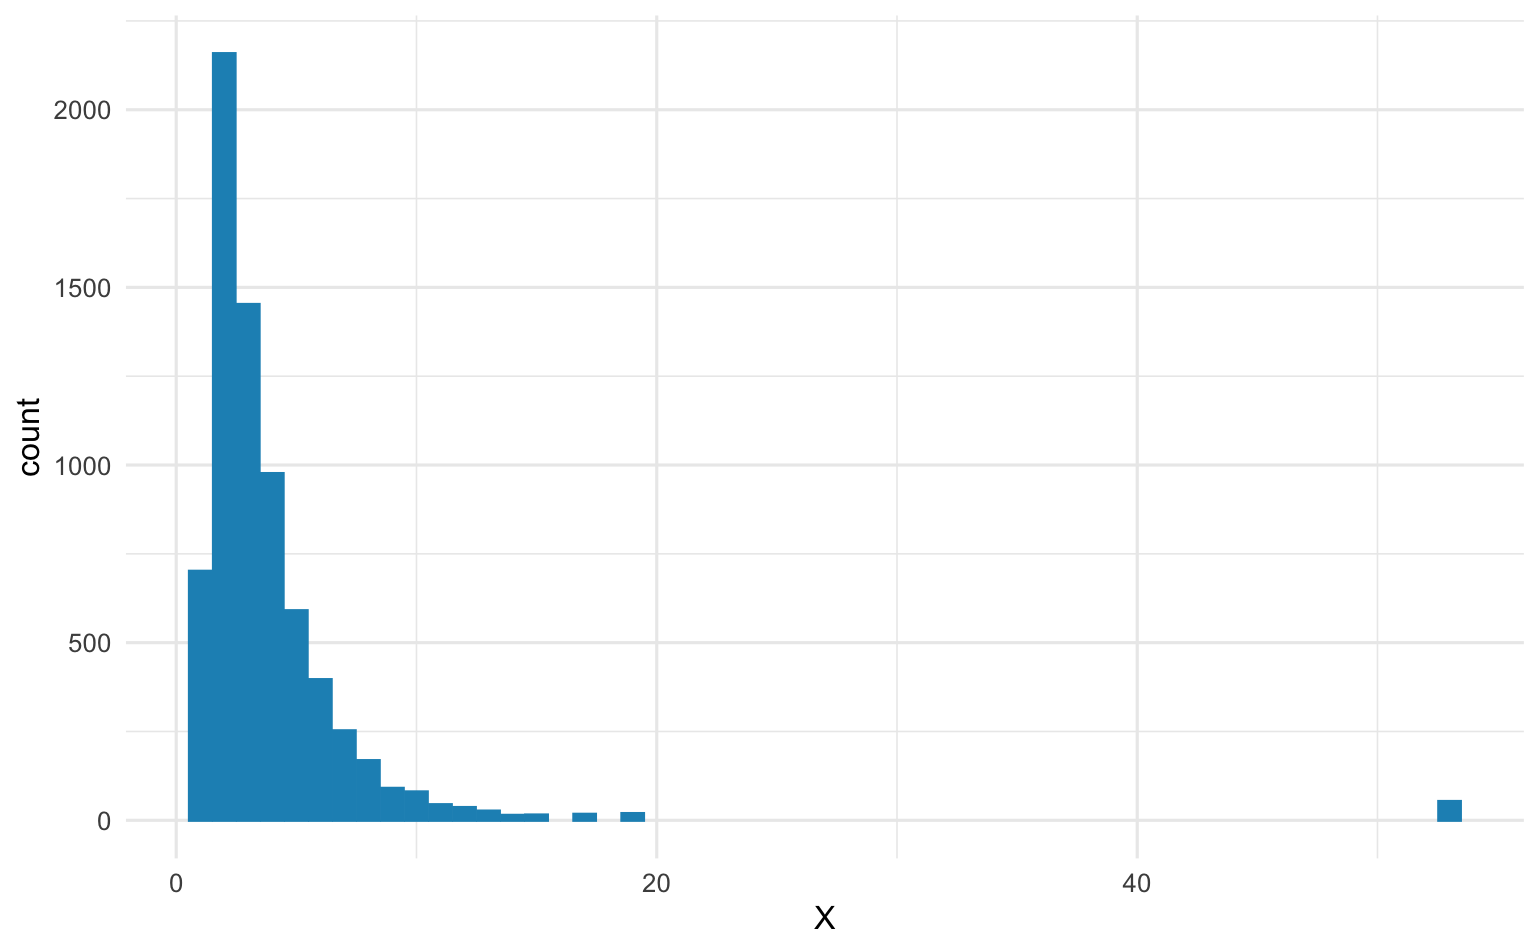
\includegraphics[width=12.5cm]{Figura1}
\end{center}
\caption{Histograma de la variable Nombre de persones}
\label{fig:F1}
\end{figure}

\begin{table}[H]
\centering
\begin{tabular}{|r|r|r|r|r|r|r|r|r|}
\hline
N.Valid & Min & Q1 & Mediana & Mitjana  & Desv. estàndar & Q3 & Max & IQR \\ \hline
7087    & 1   & 2  & 3       & 4.015098 & 4.938707       & 5  & 53  & 3   \\ \hline
\end{tabular}
\caption{Resum numeric de la variable Nombre de persones \label{table:Fig1a}}
\end{table}



Per tal d'assegurar-nos que aquesta dada no afecta al nostre anàlisi, i tenint en compte que disposem d'una base de dades molt gran, treurem aquests casos d'ambdues taules. 


\begin{figure}[H]
\begin{center}
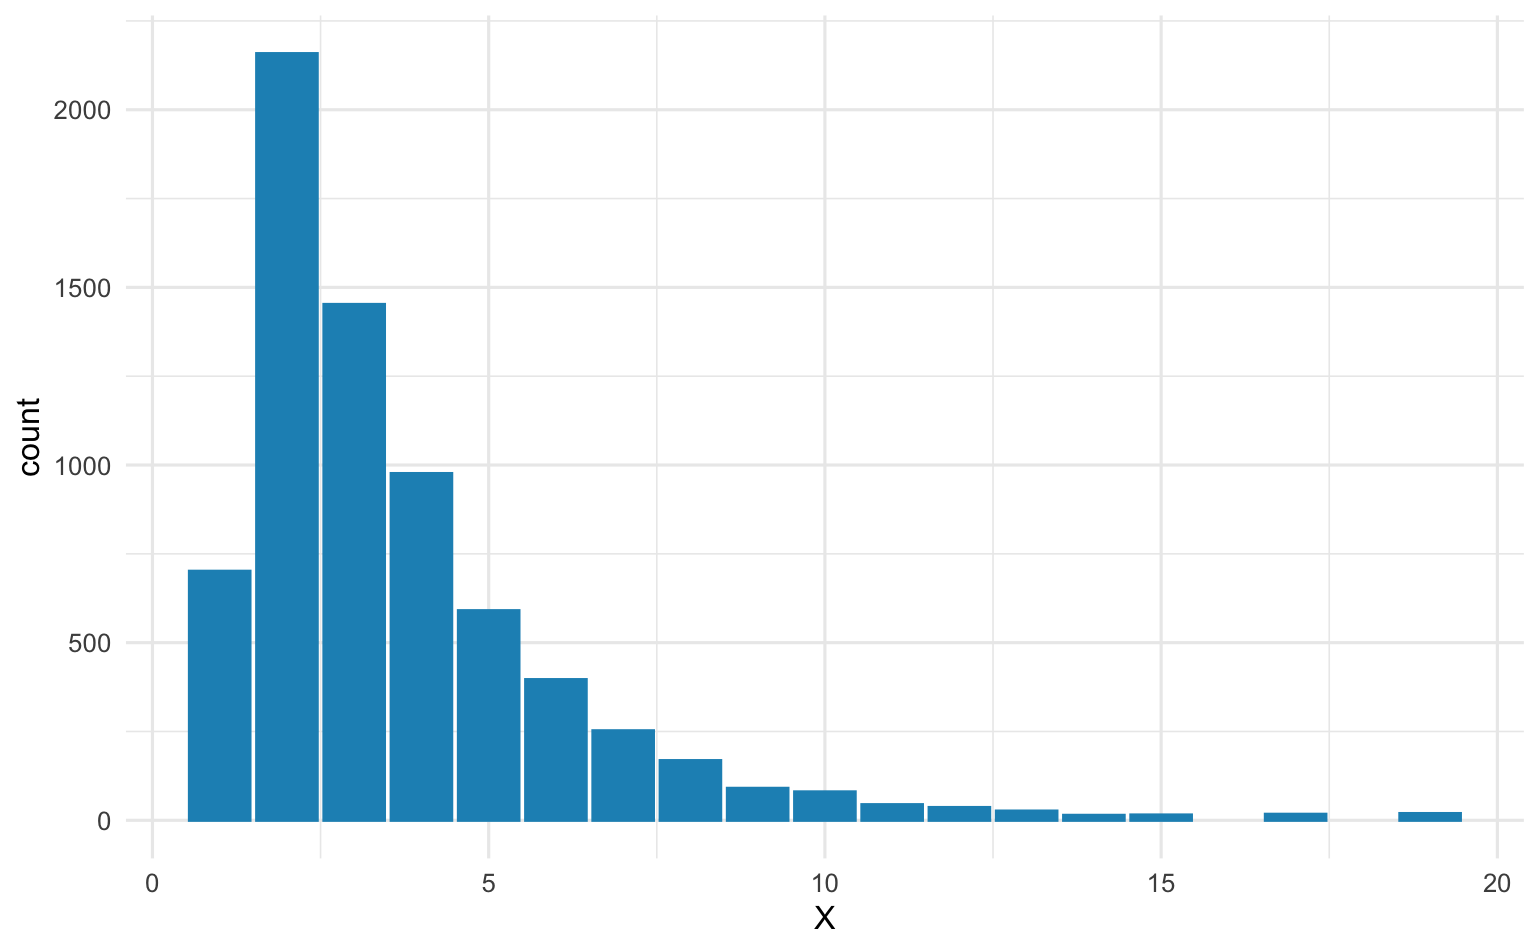
\includegraphics[width=12.5cm]{Figura2}
\end{center}
\caption{Histograma de la variable Nombre de persones després d'eliminar els outliers}
\label{fig:F2}
\end{figure}

\begin{table}[H]
\centering
\begin{tabular}{|r|r|r|r|r|r|r|r|r|}
\hline
N.Valid & Min & Q1 & Mediana & Mitjana  & Desv. estàndar & Q3 & Max & IQR \\ \hline
7034    & 1   & 2  & 3       & 3.64005 & 2.521077       & 4  & 19  & 2   \\ \hline
\end{tabular}
\caption{Resum numeric de la variable Nombre de persones}
\label{tab:Fig2-table}
\end{table}

\subsubsection{Categoritzar}

En el cas de les dades mancants que es troben en variables categòriques, el que es farà serà factoritzar-les i, seguidament, definir els nivells que presenta el factor. Així, per exemple, la variable \textbf{PER\_TYP} presenta 8 nivells que s'han d'agrupar en 3 (Conductor, Ocupant i Altres). 


A continuació es mostren els canvis realitzats a algunes de les variables categòriques de la base de dades:



\textbf{PER\_TYP}: Tipus de persona (1 = conductor, 2 = ocupant, resta de codis = altres).

\begin{itemize}

\item Abans: 1, 2, 3, 4, 5, 6, 8, 9

\item Després: Conductor, Ocupant, Altres

\end{itemize}


\textbf{DAY\_WEEK}: Dia de la setmana (1 = Diumenge, 2 = Dilluns, . . . , 7 = Dissabte).

\begin{itemize}

\item Abans: 1, 2, 3, 4, 5, 6, 7

\item Després: Diumenge, Dilluns, Dimarts, Dimecres, Dijous, Divendres, Dissabte

\end{itemize}

\textbf{SEX}: Sexe de la persona (1 = home, 2 = dona, 8 = No registrat, 9 = Desconegut).

\begin{itemize}

\item Abans: 1, 2, 8, 9

\item Després: Home, Dona

\end{itemize}

Per la variable variable \texttt{SEX} hi ha les categories anomenades "No registrat" i "Desconegut", que representen aquelles persones de les quals no tenim informació del seu sexe. Com aquestes categories no ens aporten informació d'utilitat a l'hora de realitzar l'estudi ni per a realitzar models predictius, prescindirem dels individus que corresponguin a aquestes per a realitzar el nostre anàlisi.

\textbf{RUR\_URB}: Informació sobre la localització (1 = Rural, 2 = Urbà, 6 = Via no classificada, 8 = No registrat, 9 = Desconegut). 

\begin{itemize}

\item Abans: 1, 2, 6, 8, 9

\item Després: Rural, Urbà, Desconegut

\end{itemize}


\textbf{HI HA MORTS}: Variable identificadora dels accidents mortals (0: no hi ha morts en l'accident, 1: hi ha morts en l'accident).


\begin{itemize}

\item Abans: 0, 1

\item  Després: No, Sí

\end{itemize}

\textbf{DOA}: Tipus de víctima (0 = sobreviu, 7 = mort a l’accident, 8 = mort al trasllat, 9 = Desconegut)

\begin{itemize}

\item  Abans: 0, 7, 8, 9

\item  Després: Sobreviu, Mor

\end{itemize}

Per aquesta última variable, \texttt{DOA}, hi ha una categoria anomenada "Desconegut", que representa aquelles persones que no se sap si sobreviuen a l'accident o no. Ja que en aquest estudi el fet de sobreviure o no a l'accident és de gran interès, i aquesta categoria  no ens aporta informació útil, prescindirem dels individus enmarcats en aquesta categoria per a realitzar el nostre anàlisi. A més a més, agruparem les categories 7 i 8 (mort a l'accident i mort al trasllat, respectivament) en una única categoria.

Per últim, es crearan dues variables noves a partir de \texttt{HOURS} i \texttt{DAY}, que ja són presents a ambdós conjunts de dades. Aquest pas es realitza perquè les variables \texttt{HOURS} i \texttt{DAY} tenen un rang de valors molt elevat que ens aporta poca informació. 

\textbf{HOURS\_agrupat}

En el cas de la variable \texttt{HOURS}, es tindrà en compte que, comunament, es considera que el dia està format per 5 intervals de temps segons la posició del sol. Aquest són la matinada (de les 0 a les 5 h incloses), el matí (de les 6 a les 11 h incloses), el migdia (de les 12 a les 14 h incloses), la tarda (de les 15 a les 19 h incloses) i la nit (de les 20 a les 23 h incloses). S'han fet servir aquests intervals per definir la nova variable \texttt{HOURS\_agrupat}.

\begin{itemize}

\item Abans: 0, 1, 2, 3, 4, 5, 6, 7, 8, 9, 10, 11, 12, 13, 14, 15, 16, 17, 18, 19, 20, 21, 22, 23

\item Després: Matinada, Matí, Migdia, Tarda, Nit

\end{itemize}


\textbf{SETMANA}


Pel que fa a la variable \texttt{SETMANA}, s'han definit les setmanes del mes en que es va realitzar el seguiment que presenten les dades. S'ha considerat el primer dia de la setmana el dilluns i l'últim el diumenge, tenint en compte que el dia 1 del mes era un dimarts. Per aquest motiu les setmanes 1 i 5 són les més curtes, especialment la cinquena, ja que el dia 31 va caure en dijous.


\begin{itemize}

\item Abans: 0, 1, 2, 3, 4, 5, 6, 7, 8, 9, 10, 11, 12, 13, 14, 15, 16, 17, 18, 19, 20, 21, 22, 23, 24, 25, 26, 27, 28, 29, 30, 31

\item Després: Setmana 1, Setmana 2, Setmana 3, Setmana 4, Setmana 5

\end{itemize}


\subsubsection{Variable resposta}

Per últim, definirem les variables resposta per a cada taula, és a dir, aquelles característiques que ens interessa poder predir tant en els futurs accidents com en les pròximes persones que es vegin involucrades en aquests.


Per una banda, és d'interès classificar els accidents segons si aquests han ocasionat morts o bé no ha sigut el cas. D'aquesta manera, es podria crear un model de predicció que permeti establir si un accident serà mortal o no en el futur en funció de les característiques que presenti.


Per tant, la variable d'interès és \texttt{HIHAMORTS}, que es mostra a la figura \ref{fig:F3}.

\begin{table}[H]
\centering
\begin{tabular}{llll}
\hline
Variable         & Categories  & Freqüències   & Missings \\ \hline
Hi ha morts & 1. No & 1176 (42.3\%) & 0        \\
{[}factor{]}     & 2. Sí      & 1604 (57.7\%) & (0.00\%) \\ \hline
\end{tabular}
\end{table}

\begin{figure}[h!]
\par
\raisebox{-.5\height}{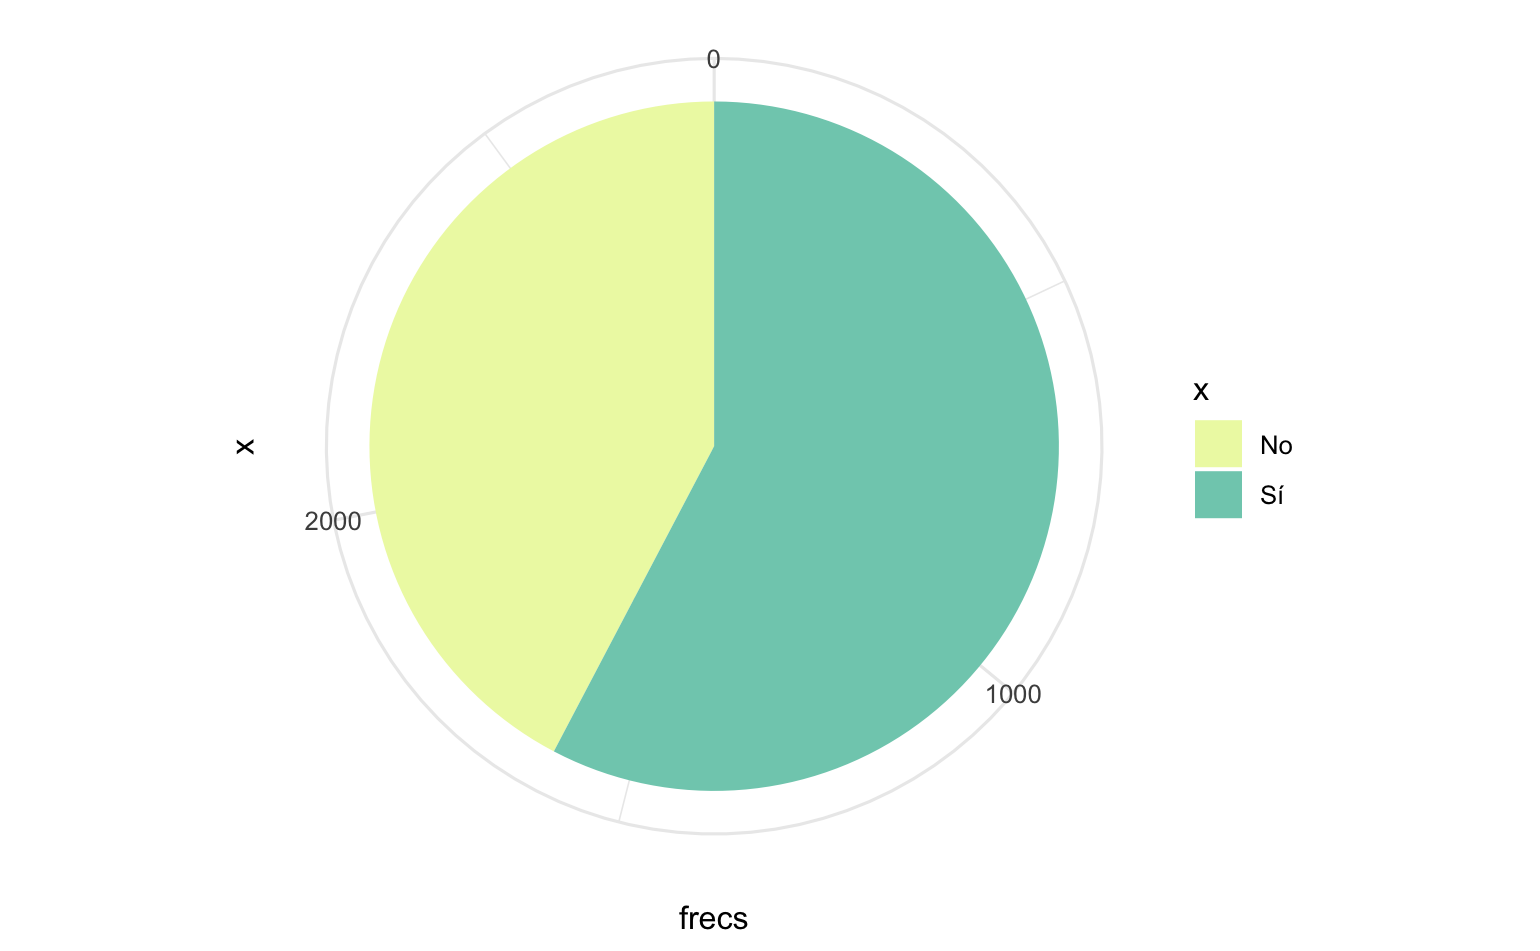
\includegraphics[width=7.25cm]{Figura3a}}%
\hfill
\raisebox{-.5\height}{
\includegraphics[width=7.25cm]{Figura3b}}%
\par

\caption{Anàlisi descriptiu de la variable Hi ha morts}
\label{fig:F3}
\end{figure}

El tant per cent d'accidents amb morts és molt elevat perquè tots són accidents amb víctimes que es van enregistrar per l'autoritat i, per tant, devia anar-hi un agent de trànsit al lloc on es va produir. Els accidents més lleus o superficials no van ser enregistrats per aquest estudi.


Seguint aquesta línia, serà també de gran importància el tipus de víctima que esdevindran cadascuna de les persones implicades en un accident. En aquest cas, la variable d'interès serà \texttt{DOA}, de la qual es pot trobar un breu anàlisi descriptiu a la figura \ref{fig:F4}.

\begin{table}[H]
\centering
\begin{tabular}{llll}
\hline
Variable         & Categories  & Freqüències   & Missings \\ \hline
Tipus de víctima & 1. Sobreviu & 5113 (74.1\%) & 0        \\
{[}factor{]}     & 2. Mor      & 1791 (25.9\%) & (0.00\%) \\ \hline
\end{tabular}
\end{table}

\begin{figure}[h!]
\par
\raisebox{-.5\height}{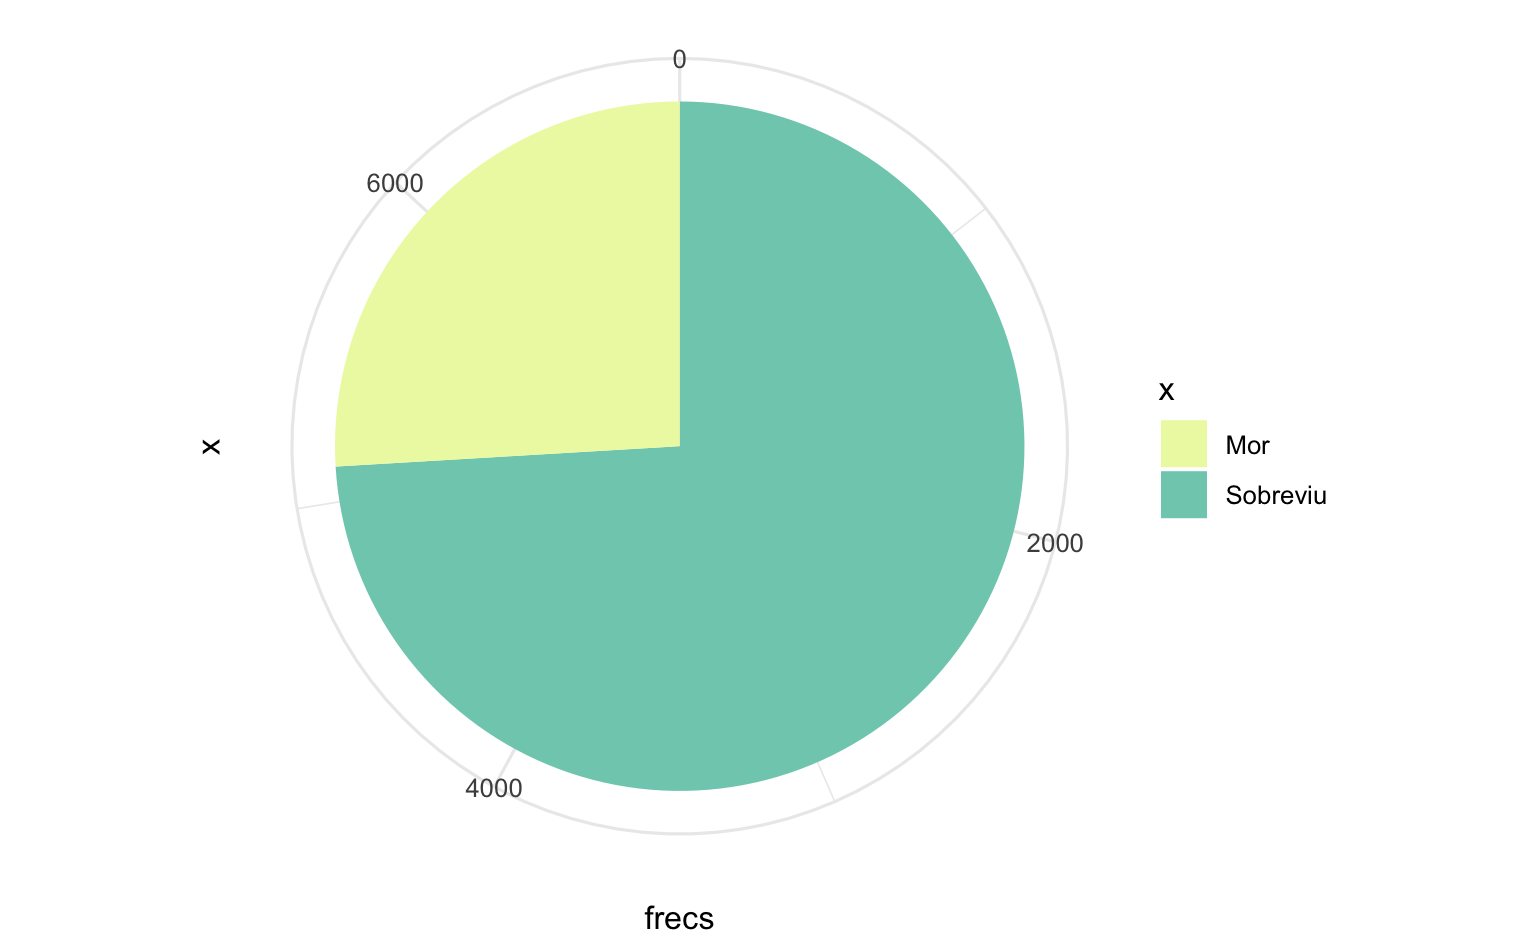
\includegraphics[width=7.25cm]{Figura4a}}%
\hfill
\raisebox{-.5\height}{
\includegraphics[width=7.25cm]{Figura4b}}%
\par

\caption{Anàlisi descriptiu de la variable Tipus de víctima}
\label{fig:F4}
\end{figure}

\newpage


\subsection{Anàlisi descriptiva}

\subsubsection{Anàlisi univariant}

\begin{large}

\textbf{Variables numèriques}

\end{large}

\textbf{Variables vinculades als accidents}


\begin{table}[H]
\centering
\begin{tabular}{lll}
\hline
Variable    & Tipus    & Descripció                                           \\ \hline
HOUR        & Numèrica & Hora de l’accident (99 = desconeguda)                \\
MINUTE      & Numèrica & Minut de l’accident (99 = desconegut)                \\
FATALS      & Numèrica & Nombre de víctimes a l’accident (poden ser ferits o morts)                      \\
DRUNK\_DR   & Numèrica & Nombre de conductors beguts involucrats a l’accident \\
MORTS       & Numèrica & Nombre de morts en l’accident                        \\
NO\_PER     & Numèrica & Nombre de persones implicades en l’accident          \\
NO\_VEHICLE & Numèrica & Nombre de vehicles implicats en l’accident           \\ \hline
\end{tabular}
\caption{Variables numeriques vinculades als accidents}
\label{tab:num-table}
\end{table}

Per a comprovar que les dades són correctes i que s'han tractat bé en termes de \emph{missings} i \emph{outliers}, farem ús del resum numèric de cada variable que es mostra a la taula \ref{tab:num2-table}. 

Les variables \texttt{HOUR} i \texttt{MINUTE} prenen valors entre 0 i 23 i entre 0 i 59 respectivament, els quals són rangs esperats i no donen peu a cap dada atípica en la seva distribució. A la tercera fila de la taula es troba el nombre de víctimes de l'accident, \texttt{FATALS}, que assenyala que no hi ha cap accident en què no hi hagi, com a mínim, una víctima. També veiem com el nombre màxim de víctimes és 5, però en termes generals i d'acord amb els quartils 1, 2 i 3 i la mitjana s'observa que la gran majoria dels accidents (el 75\%) només en presenten una. Així mateix, pel que fa al nombre de conductors beguts involucrats a l'accident, \texttt{DRUNK\_DR}, aquesta variable pren el valor 0 en la majoria dels casos (el 75\% com a mínim, com indica el tercer quartil). Això no obstant, hi ha casos en què hi ha fins a 2 conductors beguts involucrats en un mateix accident. 

\begin{table}[H]
\centering
\begin{tabular}{lrrrrrrrrr}
\hline
Variable    & N.Valid & Min & Q1 & Q2 & Mitjana    & Desv.  & Q3 & Max & IQR \\ \hline
HOUR        & 2780    & 0   & 7  & 15      & 13.0122 & 6.7949       & 18 & 23  & 11  \\ \hline
MINUTE      & 2780    & 0   & 13 & 28      & 28.0417 & 17.2255      & 43 & 59  & 30  \\ \hline
FATALS      & 2780    & 1   & 1  & 1       & 1.1000  & 0.3833       & 1  & 5   & 0   \\ \hline
DRUNK\_DR   & 2780    & 0   & 0  & 0       & 0.2457  & 0.4429       & 0  & 2   & 0   \\ \hline
MORTS       & 2780    & 0   & 0  & 1       & 0,6442  & 0.6346       & 1  & 5  & 1   \\ \hline
NO\_PER     & 2780    & 1   & 1  & 2       & 2.5302  & 1.6805       & 3  & 19  & 2   \\ \hline
NO\_VEHICLE & 2780    & 1   & 1  & 1       & 1.5079  & 0.6998       & 2  & 6   & 1   \\ \hline
\end{tabular}
\caption{Resum de les variables numèriques vinculades als accidents}
\label{tab:num2-table}
\end{table}





Per la variable \texttt{NO\_PER}, s'observa que el mínim de persones que es trobaven als vehicles en el moment de l'accident era un, cosa que té sentit, ja que no podria haver-hi cap accident de trànsit si no hi hagués, com a mínim, un conductor. La mitjana de gent implicada en cada accident va de 2 a 3 persones, i l'accident en el qual va haver-hi més participants van arribar a ser fins a 19 persones. Aquest tipus d'accident és creïble, ja que quatre cotxes poden arribar a col·lidir en una carretera si hi ha molt poc temps de reacció i, si aquests cotxes van plens, es podria arribar a parlar de vint persones en un accident, comptant que no hi hagués cap vianant.

Pel que fa a \texttt{MORTS}, es pot veure com en el 25\% dels casos, com a mínim, no hi ha cap víctima mortal en aquests accidents. La mitjana no arriba a ser un, cosa que indica que la majoria dels accidents no presenten cap mort, i en el 75\% dels casos el màxim de víctimes és d'un. Així i tot, hi ha un cas en el qual hi va haver 5 morts, que destaca per sobre de la resta. 


Per acabar, en tots els accidents de trànsit hi ha un mínim d'un vehicle, i així ho mostra la variable \texttt{NO\_VEHICLE}. L'accident amb més vehicles implicats en té 6.


Quant als \emph{missings}, la primera columna de la taula és un recompte dels casos vàlids per a cada variable, és a dir, aquells que no presenten valors mancants per a aquella variable concreta. Es pot comprovar com el mètode d'imputació s'ha realitzat correctament, perquè totes les variables presenten el mateix recompte de casos vàlids, que coincideix amb el nombre d'accidents total a la base de dades.

\textbf{Variables vinculades a les persones}

Sobre les variables vinculades a les persones (Taula \ref{tab:num3-table}), només varien les variables \texttt{NO\_FUGITS} i \texttt{EDAT} respecte a la taula anterior. De fet, la distribució de les variables \texttt{HOUR}, \texttt{MINUTE}, \texttt{FATALS}, \texttt{DRUNK\_DR}, \texttt{NO\_PER}, \texttt{MORTS} i \texttt{NO\_VEHICLE} no presenta canvis rellevants respecte a la distribució que es troba a la taula anterior. No es troba cap cas de dada atípica ni cap dada mancant per aquestes variables. Per aquest motiu, ens centrarem ara en els resums de les variables \texttt{NO\_FUGITS} i \texttt{EDAT}, que es troben a la taula \ref{tab:num4-table}.

\begin{table}[H]
\centering
\begin{tabular}{lll}
\hline
Variable    & Tipus    & Descripció                                           \\ \hline
HOUR        & Numèrica & Hora de l’accident (99 = desconeguda)                \\
MINUTE      & Numèrica & Minut de l’accident (99 = desconegut)                \\
FATALS      & Numèrica & Nombre de víctimes a l’accident  (poden ser ferits o morts)                     \\
DRUNK\_DR   & Numèrica & Nombre de conductors beguts involucrats a l’accident \\
MORTS       & Numèrica & Nombre de morts en l’accident                        \\
NO\_PER     & Numèrica & Nombre de persones implicades en l’accident          \\
NO\_VEHICLE & Numèrica & Nombre de vehicles implicats en l’accident           \\
NO\_FUGITS  & Numèrica & Nombre de vehicles fugits implicats en l’accident    \\
AGE         & Numèrica & Edat de la persona                                   \\ \hline
\end{tabular}
\caption{Variables numeriques vinculades a les persones}
\label{tab:num3-table}
\end{table}

\begin{table}[H]
\centering
\begin{tabular}{lrrrrrrrrr}
\hline
Variable    & N.Valid & Min & Q1   & Q2 & Mitjana    & Desv. & Q3 & Max & IQR   \\ \hline
HOUR        & 6904    & 0   & 8.0  & 15      & 13.4422 & 6.5239       & 18 & 23  & 10.00 \\ \hline
MINUTE      & 6904    & 0   & 13.0 & 28      & 27.8872 & 17.2487      & 43 & 59  & 30.00 \\ \hline
FATALS      & 6904    & 1   & 1.0  & 1       & 1.1705  & 0.5296       & 1  & 5   & 0.00  \\ \hline
DRUNK\_DR   & 6904    & 0   & 0.0  & 0       & 0.2219  & 0.4346       & 0  & 2   & 0.00  \\ \hline
MORTS       & 6904    & 0   & 0.0  & 1       & 0.6966  & 0.7340       & 1  & 5   & 1.00  \\ \hline
NO\_PER     & 6904    & 1   & 2.0  & 3       & 3.6548  & 2.5291       & 4  & 19  & 2.00  \\ \hline
NO\_VEHICLE & 6904    & 1   & 1.0  & 2       & 1.7784  & 0.8766       & 2  & 6   & 1.00  \\ \hline
NO\_FUGITS  & 6904    & 0   & 0.0  & 0       & 0.0529  & 0.2478       & 0  & 3   & 0.00  \\ \hline
AGE         & 6904    & 0   & 23.5 & 37      & 39.9005 & 20.4028      & 55 & 98  & 31.25 \\ \hline
\end{tabular}
\caption{Resum de les variables numèriques vinculades a les persones}
\label{tab:num4-table}
\end{table}




Pel que fa al nombre de vehicles fugits a l'accident, el tercer quartil indica que al 75\% dels casos no hi ha cap vehicle fugit, i si en fixem en el valor màxim que pren aquesta variable, el cas amb més vehicles fugits en presenta 3. Finalment, sobre l'edat de les persones, el rang de valors va des de 0 fins a 98 anys, és a dir, en alguns accidents hi ha implicats nadons, i en altres a persones de mitjana edat. 

Novament, ens trobem que la primera columna de la taula és un recompte dels casos vàlids per a cada variable, és a dir, aquells que no presenten valors mancants per a aquella variable concreta. Es pot comprovar com el mètode d'imputació s'ha realitzat correctament, perquè totes les variables presenten el mateix recompte de casos vàlids, que coincideix amb el nombre d'accidents total.



\begin{large}

\textbf{Variables categòriques}

\end{large}

\textbf{Variables vinculades als accidents}



\textbf{DAY}: Dia de l’accident (de l’1 al 31). Tipus de variable: Factor

\begin{table}[H]
\centering
\begin{tabular}{lllr}
\hline
Variable     & \multicolumn{1}{r}{Categoria} & \multicolumn{1}{r}{Freqüència} & Missings  \\ \hline
DAY          & 1. 1                          & 71 (2.6\%)                     & 0 (0.0\%) \\
{[}factor{]} & 2. 2                          & 84 (3.0\%)                     &           \\
             & 3. 3                          & 108 (3.9\%)                    &           \\
             & 4. 4                          & 96 (3.5\%)                     &           \\
             & 5. 5                          & 117 (4.2\%)                    &           \\
             & 6. 6                          & 112 (4.0\%)                    &           \\
             & 7. 7                          & 78 (2.8\%)                     &           \\
             & 8. 8                          & 81 (2.9\%)                     &           \\
             & 9. 9                          & 88 (3.2\%)                     &           \\
             & 10. 10                        & 85 (3.1\%)                     &           \\
             & {[}21 altres{]}               & 1859 (66.9\%)                  &           \\ \hline
\end{tabular}
\end{table}

La freqüència d'accidents segons el dia del mes sembla prou estable, i no es troba cap patró significatiu.


\textbf{RUR\_URB}: Informació sobre la localització (1 = Rural, 2 = Urbà, 6 = Via no classificada, 8 = No registrat, 9 = Desconegut). Tipus de variable: Factor

\begin{table}[H]
\centering
\begin{tabular}{lllr}
\hline
Variable     & \multicolumn{1}{r}{Categoria} & \multicolumn{1}{r}{Freqüència} & Missings  \\ \hline
RUR\_URB     & 1. Rural                      & 1174 (42.2\%)                  & 0  \\
{[}factor{]} & 2. Urbà                       & 1288 (46.3\%)                  &      (0.0\%)     \\
             & 3. Desconegut                 & 318 (11.4\%)                   &           \\ \hline
\end{tabular}
\end{table}

En 318 casos no hi ha informació sobre la localització de l'accident, però per la resta dels casos, el 88,6\%, es pot identificar si va ser en una zona rural o urbana, i els casos estan prou balancejats en aquestes dues categories.


\textbf{DAY\_WEEK}: Dia de la setmana (1 = Diumenge, 2 = Dilluns, . . . , 7 = Dissabte). Tipus de variable: Factor



\begin{table}[H]
\centering
\begin{tabular}{llll}
\hline
Variable & \multicolumn{1}{r}{Categoria} & \multicolumn{1}{r}{Freqüència} & \multicolumn{1}{r}{Missings} \\ \hline
DAY\_WEEK    & 1. Diumenge  & 356 (12.8\%) & \multicolumn{1}{r}{0} \\
{[}factor{]} & 2. Dilluns   & 311 (11.2\%) & \multicolumn{1}{r}{(0.0\%)}          \\
             & 3. Dimarts   & 410 (14.7\%) & \multicolumn{1}{r}{}          \\
             & 4. Dimecres  & 436 (15.7\%) &                               \\
             & 5. Dijous    & 460 (16.5\%) &                               \\
             & 6. Divendres & 387 (13.9\%) &                               \\
             & 7. Dissabte  & 420 (15.1\%) &                              \\ \hline
\end{tabular}
\end{table}

El mes de desembre de 2015 es van donar la majoria d'accidents de trànsit els dijous, mentre que el dia de la setmana on es van donar menys va ser el dilluns.

\textbf{HIHAMORTS}:  Tipus de variable: Factor


\begin{table}[H]
\centering
\begin{tabular}{llll}
\hline
Variable & \multicolumn{1}{r}{Categoria} & \multicolumn{1}{r}{Freqüència} & \multicolumn{1}{r}{Missings} \\ \hline
HIHAMORTS    & 1. No  & 1176 (42.3\%) & \multicolumn{1}{r}{0} \\
{[}factor{]} & 2. Sí   & 1604 (57.7\%) & \multicolumn{1}{r}{(0.0\%)}          \\\hline
\end{tabular}
\end{table}

Aquesta és la variable resposta de la taula, és a dir, aquella que ens interessa predir a partir de la relació amb la resta de variables de la taula. Pren dues categories (sí i no) i, pel que es pot veure, està una mica desbalancejada. Això vol dir que trobem més accidents a la taula en què hi ha hagut víctimes mortals que en què no s'hagin donat. La característica del balanceig, si no es compleix, pot ser un inconvenient a l'hora de crear el model, ja que pot donar més pes a uns casos per sobre dels altres. Tanmateix, com la diferència és petita, s'ha decidit treballar amb les dades que tenim, sense aplicar cap tècnica de balanceig que podria afectar les dades.


\textbf{Variables vinculades a les persones}


\textbf{SEX}: Sexe de la persona (1 = home, 2 = dona). Tipus de variable: Factor


\begin{table}[H]
\centering
\begin{tabular}{llll}
\hline
Variable & \multicolumn{1}{r}{Categoria} & \multicolumn{1}{r}{Freqüència} & \multicolumn{1}{r}{Missings} \\ \hline
SEX    & 1. Home  & 4569 (66.2\%) & \multicolumn{1}{r}{0} \\
{[}factor{]} & 2. Dona   & 2335 (33.8\%) & \multicolumn{1}{r}{(0.0\%)}          \\\hline
\end{tabular}
\end{table}

Per aquesta variable s'han eliminat els individus amb el sexe no registrat o desconegut, perquè són categories de la variable que no aporten informació extra sobre l'individu. Cal destacar, a més a més, que la majoria de les persones d'aquesta taula són homes (66,2\%). 

\textbf{PER\_TYP}: Tipus de persona (1 = conductor, 2 = ocupant, resta de codis = altres). Tipus de variable: Factor


\begin{table}[H]
\centering
\begin{tabular}{llll}
\hline
Variable & \multicolumn{1}{r}{Categoria} & \multicolumn{1}{r}{Freqüència} & \multicolumn{1}{r}{Missings} \\ \hline
PER\_TYP    & 1. Conductor  & 4057 (58.8\%) & \multicolumn{1}{r}{0} \\
{[}factor{]}      & 2. Ocupant  & 2096 (30.4\%) & \multicolumn{1}{r}{(0.0\%)} \\
                     & 3. Altres   & 751 (10.9\%) & \multicolumn{1}{r}{}          \\\hline
\end{tabular}
\end{table}

Quant al tipus de persona, se'n desconeix la informació d'aproximadament l'11\% dels individus, mentre que gairebé el 60\% de les persones involucrades als accidents eren conductors. Per tant, d'aquí es pot extreure que a la majoria de vehicles que van patir un accident en aquest període de temps només viatjava una persona, el conductor o conductora del vehicle.


\textbf{DOA}: Tipus de víctima (0 = sobreviu, resta de codis = mor). Tipus de variable: Factor


\begin{table}[H]
\centering
\begin{tabular}{llll}
\hline
Variable & \multicolumn{1}{r}{Categoria} & \multicolumn{1}{r}{Freqüència} & \multicolumn{1}{r}{Missings} \\ \hline
DOA    & 1. Sobreviu  & 5113 (74.1\%) & \multicolumn{1}{r}{0} \\
{[}factor{]} & 2. Mor   & 1791 (25.9\%) & \multicolumn{1}{r}{(0.0\%)}          \\\hline
\end{tabular}
\end{table}

Per acabar, pel tipus de víctima, que és la variable resposta en aquest cas, no hi ha balanceig entre les categories ``Sobreviu'' i ``Mor''. Si es vol crear un model per intentar predir la classe d'aquesta variable, molt probablement s'hauria d'emprar alguna tècnica de balanceig sobre aquestes dades.

\subsubsection{Anàlisi bivariant}


Per acabar l'anàlisi descriptiva de les dades, s'estudiarà la relació que existeix entre diferents parells de variables. Aquest tipus d'anàlisi ajudarà a esbrinar si existeix una associació entre les variables i, en cas afirmatiu, quina és la força d'aquesta.


Per a la visualització d'aquestes relacions entre variables s'ha fet d'ús d'una plataforma de Google anomenada \href{https://datastudio.google.com/overview}{Looker Studio}. Aquesta permet convertir les dades en panells o informes complets, fàcils de llegir i de compartir, així com totalment personalitzables. 


Amb Looker Studio es poden elaborar fàcilment informes sobre dades procedents d'una gran varietat de fonts, sense necessitat de programar. En tan sols uns instants, permet la connexió a grans conjunts de dades com els que es troben a BigQuery. Amb aquesta finalitat, s'han pujat les taules preprocessades altra vegada a BigQuery, i s'ha establert la connexió amb l'eina de visualització.


\textbf{Variables vinculades als accidents}


\begin{figure}[h!]
\par
\raisebox{-.5\height}{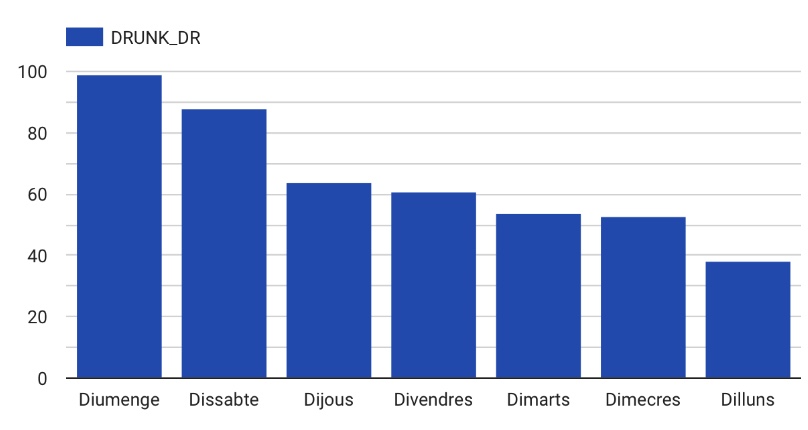
\includegraphics[width=7.5cm]{Graph1}}%
\hfill
\raisebox{-.5\height}{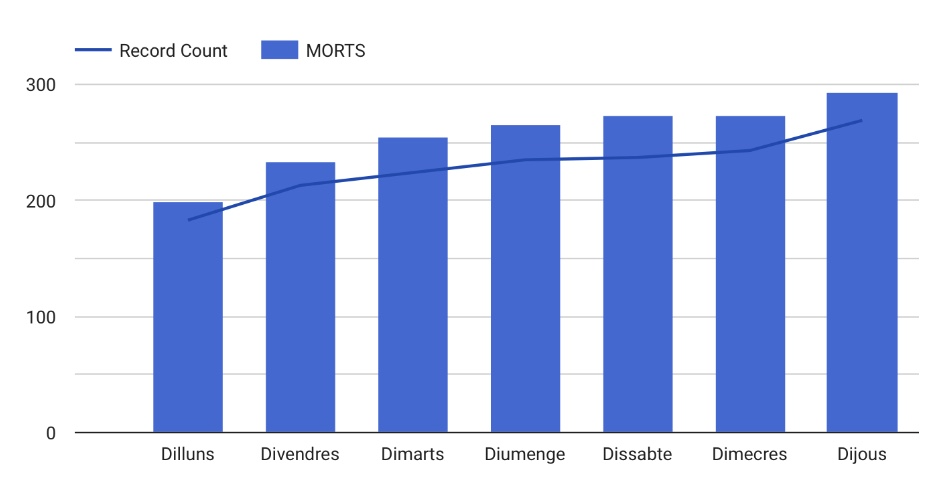
\includegraphics[width=7.5cm]{Graph2}}%
\par

\caption{Nombre de conductors beguts i quantitat d'accidents, respectivament}
\label{fig:G1}
\end{figure}

Pel que fa al nombre de conductors beguts segons el dia de la setmana en el qual succeeix l'accident, s'observa de forma clara a la gràfica esquerra de la figura  \ref{fig:G1} com la majoria dels conductors beguts es concentren al cap de setmana. Sembla que podria ser un patró perquè hi ha diferències notables entre la quantitat de conductors beguts a finals de la setmana, en comparació als dilluns, dimarts i dimecres. D'altra banda, si ens fixem, en aquest cas, en el nombre de morts segons el dia de la setmana, el dilluns es troba altra vegada en l'última posició, ja que és el dia en què es donen menys morts en accidents de trànsit. Paral·lelament, els últims dies de la setmana presenten un major nombre d'accidents mortals. Aquesta és la informació que presenta la gràfica dreta de la figura \ref{fig:G1}.


Si es té en compte la informació d'aquestes últimes gràfiques, es podria pensar que existeix una relació entre el nombre de conductors beguts i el nombre de ferits mortals als accidents de trànsit. S'haurà de tenir en compte aquesta hipòtesi per anàlisis posteriors de les dades.

\begin{figure}[h!]
\par
\raisebox{-.5\height}{\includegraphics[width=7.5cm]{Graph6}}%
\hfill
\raisebox{-.5\height}{\includegraphics[width=7.5cm]{Graph3_1}}%
\par

\caption{Hores sense agrupar i hores agrupades, respectivament}
\label{fig:G2}
\end{figure}


Si centrem l'atenció en les hores del dia, a la figura \ref{fig:G2} es poden veure les freqüències absolutes quant a la quantitat de morts en els diferents moments del dia. A l'esquerra, es divideix el dia en les seves hores, i s'observa com l'hora en què es produeixen més accidents és a les 6 de la tarda. Perquè la gràfica sigui més informativa, s'han agrupat les hores segons els moments del dia per crear la gràfica de la dreta. 


En definitiva, de les dues gràfiques s'extreu que la majoria de les morts es produeixen a la tarda i a la matinada, mentre que el moment del dia on hi ha menys morts és el migdia.


\textbf{Variables vinculades a les persones}

\begin{figure}[H]
\begin{center}
\includegraphics[width=12.5cm]{Graph12}
\end{center}
\caption{Nombre de morts quan hi ha un conductor begut a les diferents edats}
\label{fig:G3}
\end{figure}


Pel que fa a la informació que tenim registrada sobre les persones involucrades en els accidents, i en la línia de les anàlisis anteriors, la figura  \ref{fig:G3} presenta una gràfica que mostra una clara relació entre el nombre de conductors beguts i el nombre de morts en l'accident a les diferents edats de les persones implicades. Els punts més extrems d'aquesta gràfica (els que presenten major nombre de conductors beguts i, alhora, major nombre de morts) són les edats 22 i 23. Aquestes dades indueixen a pensar que hi ha més perill d'accidents mortals per a la gent jove a la carretera, si hi ha conductors beguts. Una altra manera d'interpretar aquesta gràfica podria ser que hi ha més conductors joves que agafen el cotxe havent begut i, en conseqüència, aquest grup d'edat pateix més accidents mortals.


\begin{figure}[h!]
\par
\raisebox{-.5\height}{\includegraphics[width=7.5cm]{Graph8_1}}%
\hfill
\raisebox{-.5\height}{\includegraphics[width=7.5cm]{Graph11}}%
\par

\caption{Nombre de vehicles fugits segons el dia de la setmana i segons el dia del mes, respectivament}
\label{fig:G4}
\end{figure}

El nombre de vehicles fugits en els accidents de trànsit varia en funció del moment del dia en que es produeix l'accident, així com en funció de la setmana del mes. A la figura \ref{fig:G4} es troba, a l'esquerra, la quantitat de vehicles fugits en els diferents moments del dia, i aquests es concentren sobretot a la tarda (de 15 a 19 hores, incloses) i la matinada (de les 0 a les 5 hores, incloses). En canvi, pel que fa a les diferents setmanes del mes es veu com la majoria de cotxes fugits es troben a la primera i la quarta setmana, i la distribució no és uniforme durant totes les setmanes del mes, com s'esperaria si no hi hagués cap relació entre ambdues variables.

\begin{figure}[H]
\begin{center}
\includegraphics[width=15cm]{Table1}
\end{center}
\caption{Quantitat de supervivents segons el sexe}
\label{fig:G5}
\end{figure}


En últim lloc, la figura \ref{fig:G5} mostra una taula de contingència entre les variables SEX i DOA (és a dir, el sexe de la persona i el tipus de víctima, si sobreviu o no a l'accident). Aquesta taula marca com a categoria més abundant a la base de dades els homes que sobreviuen a l'accident, i com a menys abundant les dones que no sobreviuen al mateix. 


Si es considera aquesta informació de forma relativa, aproximadament el 39\% dels homes implicats en els accidents han resultat ferits mortalment, mentre que d'entre les dones ho ha sigut aproximadament el 29\%. Tots els accidents enregistrats a la base de dades, ho són perquè en aquests hi ha hagut ferits o alguna complicació que ha portat als agents de trànsit a intervenir en aquest. Per tant, sembla haver-hi una relació en la qual els accidents que tenen algún ferit i després una víctima, aleshores és molt més freqüent que sigui un home qui mori.


\subsection{Anàlisi per components principals}


La nostra base de dades depurada té un total de 7 variables numèriques. Per tant, l'anàlisi de components principals tindrà un total de 7 components. Després de realitzar els càlculs corresponents, obtenim l'ACP de les variables numèriques a la figura \ref{fig:ACP1}.

\begin{figure}[H]
\begin{center}
\includegraphics[width=14.5cm]{acp1}
\end{center}
\label{fig:ACP1}
\end{figure}


Sabem que cada component representa una inèrcia concreta. Ho podem veure gràficament en els següent gràfic de barres (Figura \ref{fig:ACP2}).


\begin{figure}[H]
\begin{center}
\includegraphics[width=11cm]{acp2}
\end{center}
\caption{Barplot de la inèrcia de cada component}
\label{fig:ACP2}
\end{figure}


Tenint en compte que la inèrcia equival a la proporció de la variabilitat de les dades, sabem que amb un 80\% d'inèrcia, podem obtenir gairebé tota la informació. Donant un cop d'ull a la gràfica de la inèrcia, es pot veure que amb les quatre primeres components ja aconseguim gairebé el 80\% de la inèrcia, així que ens podem servir d'aquestes per la nostra anàlisi.



A continuació, realitzem un gràfic de dispersió per a totes les combinacions possibles (Figura \ref{fig:ACP3}). Diferenciarem els individus, que en el nostre cas són accidents, depenent de si hi ha hagut víctimes mortals o no en aquest. 

\begin{figure}[H]
\begin{center}
\includegraphics[width=15cm]{acp3}
\end{center}
\caption{Gràfica de la projecció dels accidents}
\label{fig:ACP3}
\end{figure}


Es pot observar que les dues primeres components no aconsegueixen diferenciar de forma clara ambdós grups, i s'esdevenen solapaments. Això no obstant, es veu una lleugera tendència dels accidents sense víctimes mortals a situar-se a valors més elevats de la segona component, i a més baixos de la primera component. 

\subsubsection{Projecció de variables numèriques}

A la gràfica corresponent a la figura \ref{fig:ACP4} es pot veure totes les variables numèriques representades en la primera i segona component.


Veiem que la majoria de variables estan representades sobre l’eix horitzontal, que correspon a la primera component. Aquestes variables són \texttt{NO\_VEHICLE}, \texttt{MORTS}, \texttt{FATALS} i \texttt{NO\_PERSONES}. A més, aquestes dues últimes prenen un valor de gairebé 0,8 i, per tant, són les que expliquen amb més precisió la primera component. Ens fixem, també, que totes aquestes variables tenen relació amb el nombre de persones, de manera que a la primera component se li pot assignar l’etiqueta de ``Nombre de persones involucrades''.

\begin{figure}[H]
\begin{center}
\includegraphics[width=12cm]{acp4}
\end{center}
\caption{Gràfica de la projecció de variables numèriques}
\label{fig:ACP4}
\end{figure}


Pel que fa a l’eix vertical, només hi ha dues variables que estiguin una mica relacionades amb la segona component. Aquestes són \texttt{HOUR} i \texttt{DRUNK\_DR}, que prenen un valor prop del 0,5. Com que a priori, aquestes dues variables no tenen gaire relació l'una amb l'altra, assignarem a la segona component l'etiqueta de ``Condicions en què es dona l'accident'', ja que a simple vista cap de les dues destaca sobre l'altre en la seva aportació a la segona component.

\begin{figure}[H]
\begin{center}
\includegraphics[width=15cm]{acp5}
\end{center}
\caption{Gràfiques de contribució de les variables a les components principals}
\label{fig:ACP5}
\end{figure}


Als gràfics de la figura \ref{fig:ACP5}, la línia vermella discontínua indica el valor mitjà de contribució. Per una determinada component, una variable amb una contribució major a aquest límit pot considerar-se important a l'hora de contribuir a aquesta component. A l'esquerra, es pot veure que les variables \texttt{NO\_PER} i \texttt{FATALS} són les que més contribueixen a la PC1, tal com s'havia destacat prèviament. D'altra banda, a la gràfica de la dreta destaca la variable \texttt{MORTS} com la més contribuent a la PC2.


Pel que fa als vectors (variables) de la Figura \ref{fig:ACP4}, ens podem fixar, també en la seva longitud i en l'angle respecte als eixos de les components principals i entre ells mateixos. 


L'angle que formen les variables \texttt{HOUR} i \texttt{DRUNK\_DR} respecte l'eix vertical és petit, la qual cosa ens indica que, tot i no ser les variables més contribuents, estan estretament relacionades amb la creació d'aquesta component. Paral·lelament, es pot dir el mateix de les variables \texttt{NO\_PER} i \texttt{FATALS} respecte a la PC1.


Una altra lectura que se li pot fer als angles entre vectors són les correlacions que mostren entre variables. D'una banda, el nombre de persones i el nombre de vehicles presenten una correlació positiva, ja que formen un angle proper a zero entre elles, així com les variables \texttt{FATALS} (nombre de víctimes) i \texttt{MORTS}. D'altra banda, però, també s'entreveu que les variables \texttt{MORTS} i \texttt{HOUR} estan incorrelacionades, és a dir, són independents l'una de l'altra, perquè formen un angle de noranta graus, així com les variables \texttt{NO\_PER} i \texttt{NO\_VEHICLE} respecte \texttt{DRUNK\_DR}.


Quant a la longitud, com major sigui la llargària d'un vector relacionat amb una variable (en un rang normalitzat del 0 a l'1), major variabilitat d'aquesta variable està continguda en la representació de les dues components representades, és a dir, millor està representada la seva informació a la gràfica. En aquest cas, \texttt{NO\_VEHICLE}, \texttt{NO\_PER}, \texttt{FATALS} i \texttt{MORTS} són les variables millor representades per les dues primeres components.


\subsubsection{Projecció de variables categòriques}


També es pot fer una projecció de les variables categòriques sobre aquestes components, si en el mateix gràfic s'afegeixen totes les categories de les variables categòriques. El resultat es pot consultar a la figura \ref{fig:ACP6}.

\begin{figure}[H]
\begin{center}
\includegraphics[width=12cm]{acp6}
\end{center}
\caption{Projecció de les variables categòriques}
\label{fig:ACP6}
\end{figure}


Clarament aquest gràfic no es pot interpretar, ja que hi ha tantes categories que no es poden distingir.
Per tant, el que es farà serà crear un gràfic per a cada variable categòrica, a veure si d'aquesta manera és més senzilla la seva interpretació.



\textbf{Variable Dia}


\begin{figure}[H]
\begin{center}
\includegraphics[width=12cm]{acp7}
\end{center}
\caption{Gràfica de la projecció de la variable Dia}
\label{fig:ACP7}
\end{figure}


Amb la variable \texttt{Dia} veiem que les categories no formen cap patró rellevant respecte a les components. N'hi ha moltes, cosa que ens dificulta veure quines són les que expliquen millor una component o altra.



\textbf{Variable Localització}

\begin{figure}[H]
\begin{center}
\includegraphics[width=12cm]{acp8}
\end{center}
\caption{Gràfica de la projecció de la variable Localització}
\label{fig:ACP8}
\end{figure}


Per la variable Localització (\texttt{RUR\_URB}) podem veure clarament que les categories ``Urbà'' i ``Rural'' expliquen la segona component, ja que són més properes a aquesta, mentre que la categoria ``Desconegut'' està més lligada a la primera component.


\textbf{Variable Dia de la setmana}

\begin{figure}[H]
\begin{center}
\includegraphics[width=12cm]{acp9}
\end{center}
\caption{Gràfica de la projecció de la variable Dia de la setmana}
\label{fig:ACP9}
\end{figure}

Per la variable Dia de la setmana (\texttt{DAY\_WEEK}) ens trobem amb que les categories que estan millor representades per les primeres components són divendres, dissabte i diumenge, ja que presenten els vectors amb major longitud. D'entre aquestes, divendres sembla més lligada a la primera component, mentre que dissabte i diumenge contribueixen de forma semblant a ambdues components.

\textbf{Variable HIHAMORTS}

\vspace{2mm}
\begin{figure}[H]
\begin{center}
\includegraphics[width=12cm]{acp10}
\end{center}
\caption{Gràfica de la projecció de la variable HIHAMORTS}
\label{fig:ACP10}
\end{figure}


Per la variable \texttt{HIHAMORTS} tenim dues categories que presenten una correlació negativa total, és a dir, si no pertany a una categoria, pertany a l'altra, evidentment. D'entre aquestes, la categoria ``NO'' queda més explicada per les primeres components, i ambdues categories contribueixen de forma igualitaria en les dues components, ja que presenten aproximadament quaranta-cinc graus respecte els dos eixos.


\textbf{Variable Hora grupada}

\begin{figure}[H]
\begin{center}
\includegraphics[width=12cm]{acp11}
\end{center}
\caption{Gràfica de la projecció de la variable Hora agrupada}
\label{fig:ACP11}
\end{figure}

Per la variable hora agrupada (\texttt{HOUR\_agrupat}) tenim cinc categories. D'entre aquestes, els accidents que queden millor explicats per les primeres components són els que es donen a la matinada. Sembla que les categories ``migdia'' i ``nit'' estan més lligades a la primera component, mentre que ``matinada'' ho està a la segona. A més, la categoria que queda menys explicada és el matí.



\textbf{Variable Setmana}

\begin{figure}[H]
\begin{center}
\includegraphics[width=12cm]{acp12}
\end{center}
\caption{Gràfica de la projecció de la variable Setmana}
\label{fig:ACP12}
\end{figure}

Per la variable \texttt{Setmana} s'aprecia que cap de les categories està gaire explicada per les primeres components, ja que els vectors són de molt poca longitud (tenen un mòdul proper a zero), i tampoc s'entreveu cap patró destacable.

\section{Aprenentatge automàtic amb BigQuery ML}

\subsection{Regressió logística}

BigQuery ML és una eina d'anàlisi que pertany a BigQuery i permet crear i executar models d'aprenentatge automàtic mitjançant consultes SQL estàndard. Com forma part de la plataforma de Google Cloud, permet continuar treballant amb les dades des del núvol, sense haver d'exportar-les localment. Aquest és un gran avantatge, ja que en funció del volum de dades que s'estiguin tractant, el fet de moure-les pot ser molt costós a escala computacional, així com restrictiu per temes d'espai. Alguns dels models compatibles amb BigQuery ML són la regressió lineal, la regressió logística (binària i multinomial), sèries temporals, arbres de decisió i xarxes neuronals profundes, entre d'altres.


Les dades que s'estan analitzant tenen com a variable resposta \texttt{HIHAMORTS}, que és una variable binària que pren el valor 1 en el cas d'haver-hi alguna víctima mortal a l'accident, i 0 altrament. En ser la variable d'interès binària, s'haurà de crear un model de classificació que ens permeti determinar si un accident tindrà víctimes mortals o no. 


La regressió logística és un enfocament estadístic que s'utilitza pels problemes de classificació, ja que permet modelar la probabilitat de què es doni una de les categories de la variable resposta (classe).


\subsubsection{Entrenament del model}

Abans de crear el model a la consola de BigQuery, dividirem la nostra base de dades en dues, les dades d'entrenament, o \emph{train}, que representaran aproximadament el 80\% del total, i les dades de prova, o \emph{test}, que en seran el 20\%. El conjunt \emph{train} s'utilitzarà per entrenar el model, mentre que \emph{test} s'utilitzarà un cop creat el model, i servirà per comprovar el bon funcionament del model. Aquesta divisió de dades sovint és emprada per evitar el sobre ajust del model, que és un problema que es dona quan un model s'ajusta massa bé a les dades d'entrenament i no aconsegueix ajustar-se de forma fiable a dades addicionals.


\begin{table}[H]
\centering
\begin{tabular}{l|ll|}
\cline{2-3}
                                   & \multicolumn{2}{l|}{Hi ha morts}     \\ \cline{2-3} 
                                   & \multicolumn{1}{l|}{0 (No)} & 1 (Sí) \\ \hline
\multicolumn{1}{|l|}{Dades totals} & \multicolumn{1}{l|}{1604}   & 1176   \\ \hline
\multicolumn{1}{|l|}{Train}        & \multicolumn{1}{l|}{1342}   & 967    \\ \hline
\multicolumn{1}{|l|}{Test}         & \multicolumn{1}{l|}{262}    & 209    \\ \hline
\end{tabular}
\label{tab:ent1}
\end{table}


Tal com s'observa a la taula, les dades estan aproximadament balancejades en els tres subconjunts. En cadascun, els accidents on hi ha víctimes mortals representen entre el 56 i el 58\% dels casos.


Per crear el model logístic a BigQuery ML, s'utilitzarà la següent sintaxi:


\begin{verbatim}
CREATE OR REPLACE MODEL [nom_projecte].[nom_base_de_dades].[nom_model] 
OPTIONS(input_label_cols=['[variable_resposta]'], model_type='logistic_reg') 
AS 
	SELECT *  EXCEPT ([variables_no_utilitzades])
	FROM `[nom_projecte].[nom_base_de_dades].[nom_taula]`;
\end{verbatim}


Es farà servir la base preprocessada a R, que s'ha importat novament a BigQuery. També cal destacar que s'ha usat totes les variables explicatives excepte les variables \texttt{MORTS}, \texttt{HOUR} i \texttt{SETMANA}. S'ha pres aquesta decisió per l'alta correlació que tenen aquestes variables amb d'altres de la mateixa taula. 

Seguidament, ajustem el model a les dades d'entrenament amb una nova consulta.


\begin{verbatim}
SELECT *
FROM ML.EVALUATE(MODEL `nom_projecte].[nom_base_de_dades].[nom_model]`, 
(
  SELECT * 
  FROM `nom_projecte].[nom_base_de_dades].train`));
\end{verbatim}


\subsubsection{Avaluació del model}



Aquest model, un cop entrenat, retorna un seguit de mètriques que fan referència a la funció de pèrdua, la duració de cada iteració i la taxa d'aprenentatge que presenta el model a cada iteració.


\begin{figure}[H]
\begin{center}
\includegraphics[width=12.5cm]{log1}
\end{center}
\caption{Entrenament del model}
\label{fig:log1}
\end{figure}


Per entendre com ha sigut l'entrenament d'aquest model, donarem un cop d'ull als resultats obtinguts.



La funció de pèrdua és un mètode per avaluar que tan bé un algoritme modela o s'ajusta a les dades d'entrenament. Si les prediccions es desvien massa dels resultats reals, la funció de pèrdua pren valors elevats. En canvi, si té l'ajuda d'una funció d'optimització, la funció de pèrdua aprèn a reduir l'error de predicció a cada iteració. En aquest sentit, en el nostre model no es redueix prou l'error de predicció, ja que comencem amb un valor de 0,684 abans de començar les iteracions, i acabem amb 0,636 a la cinquena iteració.



La següent mètrica que es troba és la duració de les iteracions. Aquest és un procés àgil en el qual la iteració que ha ocupat més temps ha sigut de 1,78 segons, aproximadament. Això, a escala d'usuari és molt atractiu, ja que permet el modelatge ràpid del model en conjunts de dades grans, cosa que normalment pot ser una limitació.



En últim lloc, es troba la taxa d'aprenentatge o \emph{learning rate}. Aquest valor es calcula mitjançant l'algoritme de descens del gradient, i afecta la velocitat en què aquest algoritme convergeix en les ponderacions òptimes pels paràmetres. Una taxa d'aprenentatge massa elevada podria impedir que les ponderacions arribin a les ponderacions òptimes, mentre que una taxa petita podria requerir moltes iteracions per calcular les ponderacions.



Seguidament, es pot avaluar el rendiment del model a partir de les dades de prova (\emph{text}). Es fa servir una consulta com l'anterior, però aquest cop dirigida aquesta altra taula de dades. En aquest cas el model retorna un seguit de mètriques i uns gràfics que permeten l'avaluació del model amb les noves dades.



Una de les primeres mètriques que trobem és la precisió del model, que és el tant per cent de les dades que s'han classificat correctament. Aquesta mètrica pren valors entre 0 i 1, i en el nostre cas és de 0,6336, és a dir, el model ha predit en el 63,36\% de les dades la classe correcta de la variable resposta. 



La mesura de recuperació fa referència al tant per cent de les dades classificades correctament d'entre les que la resposta correcta era positiva. Aquesta mètrica pren el valor de 0,8178, i significa que d'entre els casos positius (accidents amb víctimes mortals), el 81,78\% s'han classificat efectivament com a positius. Al contrari, l'exactitud (o \emph{accuracy}) quantifica el nombre d'elements classificats correctament d'entre aquells que s'han classificat com a positius i, en aquest cas, el valor baixa a 0,6228.



D'altra banda, la puntuació F1 es calcula a través de la mitjana harmònica entre les mètriques de precisió i recuperació, S'utilitza la mitjana harmònica en comptes de l'aritmètica perquè aquesta té la propietat de comportar-se com la mitjana harmònica si els valors són molt semblants, però s'apropa més cap al valor petit quan hi ha diferències entre les dues mesures.


\begin{figure}[H]
\begin{center}
\includegraphics[width=16cm]{log2}
\end{center}
\caption{Avaluació del model}
\label{fig:log2}
\end{figure}



Per acabar, es troben les mètriques de pèrdua logística (\emph{log loss}) i àrea sota la corba ROC (AUC). La corba ROC és un gràfic que mostra el rendiment d'un model de classificació en tots els llindars de classificació, presentant la taxa de falsos positius a l'eix d'abscisses i la de veritables positius a l'eix d'ordenades. L'AUC mesura l'àrea sota la corba d'aquest model i, segons el valor que prengui es pot saber com és el model:



\begin{itemize}

\item 0,5 - 0,6: El model és molt dolent

\item 0,6 - 0,7: El model és dolent

\item 0,7 - 0,8: El model és bo

\item 0,8 - 0,9: El model és molt bo

\item 0,9 - 1: El model és excel·lent

\end{itemize}



El valor de l’AUC es pot interpretar de la següent manera: donat un parell d’individus (accidents), un amb resposta positiva (Y = 1, hi ha víctimes mortals) i un altre amb resposta negativa (Y = 0, no hi ha víctimes mortals), es té un 69\% de probabilitats que l'accident on sí que hi ha hagut víctimes tingui una probabilitat predita pel model superior a la probabilitat predita per a l'accident amb resposta negativa.



La pèrdua logística, per la seva banda, és un indicador de què tan a prop està la probabilitat de predicció del valor real corresponent i, per tant, pren valors del 0 a l'1. Com més s'apropi la probabilitat predita al valor real, major serà el valor de la pèrdua logística. En aquest model pren el valor de 0,6871.



\textbf{Llindar de prediccions}



A la dreta de la figura s'hi troba una sèrie de mètriques. Per una banda, s'identifica que la classe positiva és la categoria ``Sí'', de la variable \texttt{HIHAMORTS}, mentre que la classe negativa és ``No'', i també s'hi troben altra vegada les mesures de precisió, recuperació, exactitud i puntuació F1. L'única cosa que canvia és el llindar de classe positiva, que es pot modificar a conveniència per l'usuari.



Per decidir a quina classe pertany un individu es pot establir un llindar. En funció d'aquest llindar, la probabilitat estimada obtinguda classifica les observacions. El valor per defecte que apareix a la figura és de 0,3527, i implica que tots els individus que tinguin una probabilitat de resposta positiva d'aquest valor o més alt es classificaran com a positius. Aquest és el valor mínim en el nostre cas, perquè no hi ha cap individu pel qual s'hagi calculat una probabilitat menor. Si ens fixem en la corba ROC, es veu que amb aquest valor de llindar, els falsos positius estan presents en el 100\% dels casos, perquè cap individu s'ha classificat a la classe negativa. Si movem el valor del llindar, veurem com canvien les mètriques d'avaluació del model i en quin punt de la corba ens situem.

En el cas de la classificació logística binària, totes les mètriques reflexen els valors calculats quan el llindar es fixa en 0.5.

\subsubsection{Interpretació del model}


La interpretació dels pesos o coeficients beta calculats a la regressió logística és diferent de la interpretació dels pesos de la regressió lineal, ja que el resultat de la regressió logística és una probabilitat i, per tant, pren valors entre el 0 i l'1. La suma ponderada dels paràmetres es transforma, a través de la funció logística, en una probabilitat.

\begin{center}

$log \left( \frac{P(y = Si)}{P(y = No)} \right) = \beta_0 + \beta_1 x_1 + ... + \beta_p x_p$

\end{center}

On $p$ és el nombre de paràmetres que conformen el model.



Al terme esquerre de la igualtat se l'anomena \emph{log-odds}. Els \emph{odds}, que és l'equació que es troba dins del logaritme són la probabilitat de resposta positiva entre la probabilitat de resposta negativa. Podem entendre el model logístic com un model lineal pels \emph{log-odds}, ja que a través la combinació de termes es pot quantificar com canvia la classificació o la predicció en modificar alguna de les variables. Per fer-ho, s'haurà de treballar amb els exponents de la funció anterior.

\begin{center}

$\frac{P(y = Si)}{P(y = No)}  = e^{ \beta_0 + \beta_1 x_1 + ... + \beta_p x_p)}$

\end{center}



Si canviem el valor d'una d'aquestes variables, per exemple augmentant en una unitat el valor de la variable $x_1$, es pot calcular l'odds ratio de les dues prediccions:

\begin{center}

$\frac{odds_{x_1 + 1}}{odds} = \frac{e^{ \beta_0 + \beta_1 (x_1 + 1) + ... + \beta_p x_p)}}{e^{ \beta_0 + \beta_1 x_1 + ... + \beta_p x_p)}}$

\vspace{2mm}

$\frac{odds_{x_1 + 1}}{odds} = e^{\beta_1}$

\end{center}


Un canvi en una variable d'una unitat augmenta el log-odds tant com el valor del seu pes assignat.

\begin{figure}[H]
\begin{center}
\includegraphics[width=15cm]{log3a}
\end{center}
\caption{Coeficients del model}
\label{fig:log3}
\end{figure}


Per entendre l'efecte del pes de les variables del model en la probabilitat de resposta positiva, el primer que farem serà mirar l'intercept ($\beta_0$). Quan totes les variables numèriques prenen el valor zero i les variables categòriques estan en la categoria de referència, les probabilitats estimades de resposta positiva són $e^{\beta_0} = e^{-1,0228353} = 0,3595739934$. Les categories de referència de les variables categòriques són ``urbà'', pel que fa a la informació de la localització, ``Dissabte'' (en el cas de dies de la setmana) i ``Tarda'', per la variable d'hores agrupades.

Pel que fa a les variables numèriques, que són \texttt{MINUTE}, \texttt{FATALS}, \texttt{DRUNK\_DR}, \texttt{NO\_PER} i \texttt{NO\_VEHICLE}, tenim que l'augment del valor de cada variable en una unitat afecta les probabilitats estimades en un factor de $e^{\beta_i}$, on $i$ és el subíndex de cada variable numèrica.


En el cas de \texttt{FATALS}, per exemple, es troba una relació positiva entre el nombre de víctimes a l'accident i el fet d'haver-hi hagut alguna mort en el mateix. Per cada augment unitari en el nombre de víctimes, la probabilitat de classe positiva canvia en un factor de $e^{0,79631994} = 2,217365856$.


Altrament, les variables categòriques, \texttt{RUR\_URB}, \texttt{DAY\_WEEK} i \texttt{HOUR\_agrupat} s'interpreten de forma que, canviar la variable $x_i$ de la categoria de referència a una de les altres afecta les probabilitats estimades en un factor de $\beta_i$.


Si ens fixem en la variable \texttt{RUR\_URB}, es pot calcular que si, en comptes d'ubicar-se l'accident en una zona urbana, s'ha donat en una localització rural, la probabilitat canvia en un factor de $e^{0,4165228} = 1,519911759$, mentre que si la zona és desconeguda, el canvi és de $e^{-0,0342466} = 0,9663331775$.


\newpage

\section{Conclusions}
fgfg

\newpage

%\nocite{*}

\begin{thebibliography}{99} 


\bibitem{Comtois} Comtois, D. (2021). Package 'summarytools'. \textit{Tools to Quickly and Neatly Summarize Data}. URL \url{https://CRAN.R-project.org/package=summarytools}. R package version 1.0.0. 

\bibitem{Cooksey} Cooksey, B. (2014). An Introduction to APIs. \textit{Zapier, Inc. Cvetojevic, S. Juhasz, L., \& Hochmair, H. (2016). Positional Accuracy of Twitter and Instagram Images in Urban Environment}. URL \url{https://Doi.Org/10.1553/Giscience2016_01_s191}.

\bibitem{Azuela} Skoglund, K. (2019). ``Git Essential Training: The Basics''.  LinkedIn Learning. URL \url{https://www.linkedin.com/learning/git-essential-training-the-basics}.

\bibitem{Quickstarts} Google. n.d. ``Quickstarts | BigQuery | Google Cloud.'' \textit{Google}. URL \url{https://cloud.google.com/bigquery/docs/quickstarts}.

\bibitem{sqldf} Grothendieck, G., \& Grothendieck, M. G. (2017). Package 'sqldf'. \textit{Manipulate r Data Frames Using SQL}. URL \url{https://CRAN.R-project.org/package=sqldf}. R package version 0.4-11.

\bibitem{Alboukadel} Kassambara, A., \& Mundt, F. (2020). Package 'factoextra'. \textit{Extract and Visualize the Results of Multivariate Data Analyses}. URL \url{https://CRAN.R-project.org/package=factoextra}. R package version 1.0.7. 

\bibitem{VIM} Kowarik, A., \& Templ, M. (2016). Imputation with the R Package VIM. \textit{Journal of Statistical Software} 74, 1–16. doi:10.18637/jss.v074.i07. 

\bibitem{Lakshmana} Lakshmanan, V., \& Tigani, J. (2019). \textit{Google BigQuery: The Definitive Guide: Data Ware-housing, Analytics, and Machine Learning at Scale}. O’Reilly Media.

\bibitem{Ohri} Ohri, A. (2014). \textit{R for Cloud Computing: An Approach for Data Scientists}. Springer.

\bibitem{Looker} Rischin, J. (2022). ``Looker Studio for Beginners''. LinkedIn Learning. URL \url{https://www.linkedin.com/learning/google-data-studio-for-beginners-2022}.

\bibitem{dbi} Wickham, H., \& Müller, K. (2022). Package 'DBI'. \textit{RDatabase Interface}. URL \url{https://CRAN.R-project.org/package=DBI}. R package version 1.1.3. 

\bibitem{Wickham1} Wickham, H., \& Bryan, J. (2022). Package 'bigrquery'. \textit{An Interface to Google’s ’BigQuery’ ’API’}. URL \url{https://CRAN.R-project.org/package=bigrquery}. R package version 1.4.1.

\bibitem{Wickham}  Wickham, H., Averick, M., Bryan, J., Chang, W., McGowan, L. D. A., François, R., ... \& Yutani, H. (2019). Welcome to the tidyverse. \textit{Journal of Open Source Software}, 4(43), 1686. doi: 10.21105/joss.01686 (URL: \url{https://doi.org/10.21105/joss.01686}).

\bibitem{Xie} Xie, Y. (2022). Package 'knitr'. \textit{A General-Purpose Package for Dynamic Report Generation in R}. R package version 1.41.

\bibitem{Zhu} Zhu, H. (2021). Package 'kableExtra'. \textit{Construct Complex Table with 'kable' and Pipe Syntax}. URL \url{https://CRAN.R-project.org/package=kableExtra}. R package version 1.3.4.  

\end{thebibliography} 


\newpage

\section{Annex}

(Repositori de Github)

\url{https://github.com/AnnaSalazar/TFG}


%\newpage

%\listoffigures

%\newpage

%\listoftables


\end{document}
